% !TEX program = xelatex
\documentclass[12pt,a4paper]{article}

% ── Packages ─────────────────────────────────────────────────────
\usepackage[utf8]{inputenc}
\usepackage[T1]{fontenc}
\usepackage[numbers]{natbib}
\usepackage[english]{babel}
\usepackage{amsmath, amssymb, amsthm}
\usepackage{mathtools}
\usepackage{geometry}
\usepackage{booktabs}
\usepackage{array}
\usepackage{longtable}
\usepackage{graphicx}
\usepackage{xcolor}
\usepackage{setspace}
\usepackage{titlesec}
\usepackage{abstract}
\usepackage{enumitem}
\usepackage{fancyhdr}
\usepackage{float}
\usepackage{caption}
\usepackage{subcaption}
\usepackage{tcolorbox}
\usepackage{mdframed}
\usepackage{iftex}
\usepackage{fontspec}
\setmainfont{TeX Gyre Termes}
\usepackage{tikz}
\usepackage{array, tabularx, colortbl}
\usetikzlibrary{calc}

\newtcolorbox{keyeq}{
	enhanced, breakable,
	colback=white, colframe=fxgray,
	boxrule=0.6pt, arc=2pt,
	left=6pt, right=6pt, top=4pt, bottom=4pt
}

% ── Path to figures ───────────────────────────────────────────
% Extract Graphs.rar into a subfolder "graphs/" placed next to
% this .tex file before compiling.
\graphicspath{{graphs/}{graphs_new/}}

% ── Geometry ────────────────────────────────────────────────────
\geometry{
	a4paper,
	top=2.5cm, bottom=2.5cm,
	left=3cm, right=3cm
}

% ── Colors ─────────────────────────────────────────────────────
\definecolor{fxnavy}{RGB}{0,51,102}
\definecolor{fxgray}{RGB}{90,90,90}
\definecolor{fxlight}{RGB}{230,240,255}
\definecolor{warnyellow}{RGB}{255,200,0}
\definecolor{okgreen}{RGB}{0,128,64}

% ── Cover page colors ───────────────────────────────
\definecolor{docblue}{RGB}{22,74,140}
\definecolor{doclight1}{RGB}{213,227,245}
\definecolor{doclight2}{RGB}{231,240,251}
\definecolor{docgrey}{RGB}{90,90,90}
\usepackage[colorlinks = true, urlcolor = black, linkcolor = red]{hyperref}
%\usepackage{tikz} % For the frame
%\usetikzlibrary{calc}

% ── Hyperlinks ───────────────────────────────────────────────────
\hypersetup{
	colorlinks=true,
	linkcolor=fxnavy,
	citecolor=fxnavy,
	urlcolor=fxnavy,
	pdftitle={Predicting a Bitcoin Price Range: An Out-of-Sample Test},
	pdfauthor={Armand Zewu Y. I.}
}

% ── Header / Footer ───────────────────────────────────────
\pagestyle{fancy}
\fancyhf{}
\fancyhead[L]{\small\textcolor{fxgray}{Predicting a Bitcoin Price Range}}
\fancyhead[R]{\small\textcolor{fxgray}{\thepage}}
\renewcommand{\headrulewidth}{0.4pt}

% ── Spacing ───────────────────────────────────────────────────
\onehalfspacing

% ── Boxes ─────────────────────────────────────────────────────
\tcbuselibrary{skins,breakable}
\newtcolorbox{fxbox}[1][Contributions]{
	enhanced, breakable,
	colback=fxlight, colframe=fxnavy!60!black,
	fonttitle=\bfseries %\color{fxnavy}
	,title={#1}, arc=3pt
}
\newtcolorbox{limitbox}{
	enhanced, breakable,
	colback=yellow!10, colframe=orange!70!black,
	fonttitle=\bfseries, title={Documented limitation},
	arc=3pt
}
\newtcolorbox{corrbox}[1][Error identified and corrected]{
	enhanced, breakable,
	colback=red!5, colframe=red!60!black,
	fonttitle=\bfseries, title={#1},
	arc=3pt
}

\newtcolorbox{econbox}[1][Economic interpretation]{
	enhanced, breakable,
	colback=okgreen!8, colframe=okgreen,
	fonttitle=\bfseries, title={#1},
	arc=3pt
}



% ── Notation ─────────────────────────────────────────────────────
\newcommand{\R}{\mathbb{R}}
\newcommand{\Prob}{\mathbb{P}}
\newcommand{\E}{\mathbb{E}}

\setlength{\headheight}{13.59999pt}

% marker for items that still need a result or a check
\newcommand{\todo}[1]{{\color{red}\textbf{[TODO: #1]}}}

% ---- Title page content ("SKDE-notat" style) ----
\newcommand{\titrerapport}{Predicting a Bitcoin \\Price Range: \\An Out-of-Sample Test}
%\newcommand{\soustitrerapport}{Quantitative modeling \\of EUR/USD exchange rate volatility}}
\newcommand{\resumerapport}{An out-of-sample application of a Markov-switching GARCH price-range pipeline, built on EUR/USD, to BTC-USD (2018--2026).}

% ═════════════════════════════════════════════════════════════════

\begin{document} 
% ═════════════════════════════════════════════════════════════════

% ── Cover page (integrated FX-Cover code, A4 scale 21x29.7) ──
\newgeometry{margin=0cm}
\pagestyle{empty}
\thispagestyle{empty}
\noindent


\begin{titlepage}
	\thispagestyle{empty}
	
\definecolor{localblack}{HTML}{1B3A66}      % bas du dégradé
\definecolor{localdarkgray}{HTML}{244B80}   % inutilisé
\definecolor{localmidgray}{HTML}{2C5F9E}    % haut du dégradé
	\begin{tikzpicture}[remember picture,overlay]
		
		% FOND EN DÉGRADÉ NOIR / GRIS FONCÉ
		\shade[top color=localmidgray, bottom color=localblack] 
		([shift={(-1cm,1cm)}]current page.north west) 
		rectangle 
		([shift={(1cm,-1cm)}]current page.south east);
		
		% Motif de barres verticales translucides blanches
		\foreach \x/\w/\h/\op in {
			0.5/2.2/9.5/0.12, 2.7/1.5/12/0.08, 4.2/3.2/7.8/0.15, 7.4/1.0/11/0.06, 
			8.4/2.4/10.5/0.1, 10.8/2.6/8.2/0.14, 13.4/1.8/11.8/0.08, 15.2/2.2/9.0/0.12,
			17.4/1.8/10.5/0.09
		} {
			\fill[white, opacity=\op] 
			([xshift=\x cm]current page.north west) 
			rectangle 
			([xshift=\x cm + \w cm, yshift=-\h cm]current page.north west);
		}
		
		% Bloc Institutionnel (Haut Gauche)
		\node[anchor=north west, align=left, text=white] at ([shift={(2.0cm,-2.0cm)}]current page.north west) {
			{\fontsize{14}{18}\selectfont\bfseries UNIVERSITÉ DE LOMÉ}\\[3pt]
			{\fontsize{11}{14}\selectfont\color{white!100} Faculty of Economics and Management Sciences (FASEG)}\\[2pt]
			{\fontsize{10}{13}\selectfont\color{white!100} Department of Economics}
		};
		
		% Badge Document (Haut Droite)
		%\node[anchor=north east, fill=white!15, text=black, rounded corners=2pt, inner xsep=8pt, inner ysep=5pt, font=\scriptsize\bfseries] 
		%at ([shift={(-2.0cm,-2.0cm)}]current page.north east) {
		%	INDEPENDENT RESEARCH PAPER
		%};
		
		% Titres et Auteur (Centre Gauche)
		\node[anchor=west, text width=16.5cm, align=left] at ([shift={(2.0cm,-0.5cm)}]current page.west) {
			{\fontsize{25}{25}\selectfont\bfseries\color{white} Predicting a Bitcoin \\Price Range: \vspace{0.2cm}
				\\An Out-of-Sample Test}\\[0.4em] 
			{\fontsize{20}{26}\selectfont\color{white!95} An out-of-sample application of a Markov-switching GARCH pipeline, built on EUR/USD, to BTC-USD, 2018--2026.}\\[1.8cm]
			
			{\fontsize{16}{20}\selectfont\bfseries\color{white} Armand Zewu Yawo Isaac.}\\[4pt]
			{\fontsize{11}{15}\selectfont\color{white!85} Undergraduate Student in International Economics}
		};
		
		% Encadré Mots-clés / JEL (Bas Gauche)
		\node[anchor=south west, text width=12.5cm, align=left] at ([shift={(2.0cm,6.2cm)}]current page.south west) {
			\begin{tcolorbox}[
				colback=white!10, 
				colframe=white!40, 
				arc=3pt, 
				boxrule=0.6pt, 
				left=8pt, right=8pt, top=6pt, bottom=6pt
				]
				{\footnotesize\color{black}\textbf{Keywords:} Bitcoin, Markov-switching GARCH, price range, interval forecast, out-of-sample backtesting, heavy tails, time-series econometrics}\\[3pt]
				{\footnotesize\color{black}\textbf{JEL Classification:}  C22, C32, C53, C58, F31, G17}
			\end{tcolorbox}
		};
		
		% Pied de page (Bas Gauche)
		\node[anchor=south west, text=white!90, font=\small] at ([shift={(2.0cm,2.0cm)}]current page.south west) {
			\textbf{Lomé, Togo} \quad\textbullet\quad   Quantitative Working Paper \\[3pt]
			
		};
		
		% Année (Bas Droite)
		\node[anchor=south east, fill=white!20, text=black, font=\large\bfseries, rounded corners=3pt, inner xsep=10pt, inner ysep=5pt] 
		at ([shift={(-2.0cm,2.0cm)}]current page.south east) {
			2026
		};
		
	\end{tikzpicture}
\end{titlepage}




\clearpage
\restoregeometry

\setlength{\emergencystretch}{3em}
\newpage
% ── AI Disclosure ───────────────────────────────────────────────
\begin{center}
	{\LARGE\bfseries AI Disclosure Statement}
\end{center}
\vspace{0.8cm}

During the preparation of this work, I used Claude (Anthropic) to assist with the translation of the manuscript from French to English, with the initial drafting of the R and Python code (GARCH, Markov-Switching GARCH, backtest and benchmark scripts), and as a critical reviewer of the study design and of the results. After using this tool, the output was reviewed and edited as needed, and I take full responsibility for the content of this publication.

\newpage

% ── Abstract (written last) ─────────────────────────────────────
\begin{center}
	\begin{mdframed}[backgroundcolor=fxlight,linecolor=fxnavy,linewidth=1pt,innerleftmargin=12pt,innerrightmargin=12pt,innertopmargin=10pt,innerbottommargin=10pt]
		\textbf{Abstract.}
		This paper applies, out of sample, a Markov-switching GARCH price-range pipeline built on EUR/USD to Bitcoin, an asset with no institutional anchor. It asks whether a one-day price range can be built and calibrated, and what an analyst of the market can use it for. A GARCH(1,1) with Student's~$t$ innovations ($\hat\nu\approx3.18$, persistence at the IGARCH boundary) is estimated on daily BTC-USD log returns (\texttt{yfinance}, 2014--2026, $n=4\,394$). A two-regime Markov-switching GARCH (Haas, Mittnik \& Paolella, 2004) finds persistent regimes (expected durations of about 73 and 36 days) rather than a single era, according to a rule frozen before estimation (51 switches; the longest volatile block covers $15.4\,\%$ of the sample); a split-sample test does not support the explanation of the near-unit persistence by one level shift. The one-day $95\,\%$ price range is validated by an expanding-window backtest of 3,193 forecasts over 2018--2026 (coverage $95.11\,\%$; Wilson interval $94.3$--$95.8\,\%$; Kupiec $p=0.766$; Christoffersen $p=0.610$) and, qualitatively, through the shock of March 2020 with the model frozen (121 days, $95.87\,\%$). The success criterion is weakly discriminating: a filtered historical simulation passes it with a band of the same width, and the regime layer improves the interval score by only $1.6$ to $4.2\,\%$, solidly against one reference. Coverage does not measure the size of breaches (the log return of $-46.5\,\%$ on 12 March 2020 is $6.6$ times its bound); the regime labels are relative to each re-estimation; direction is not exploitable with three simple signals. Each step is documented with its limitations and with what was fixed before and after seeing the data.
	\end{mdframed}
\end{center}

\newpage
\tableofcontents
\newpage

% ═════════════════════════════════════════════════════════════════
\section{Introduction}
\label{sec:intro}
% ═════════════════════════════════════════════════════════════════

\subsection{Objective}

The companion EUR/USD paper \citep{ZEWU2026fx} builds a chain of quantitative tools: log returns, a GARCH model, a Markov-switching GARCH with two volatility regimes, a one-day price range, and an out-of-sample validation of that range. This paper applies the same chain, with declared adaptations, to a very different asset: Bitcoin (BTC-USD), over 2014--2026, with the backtest running from 2018 to 2026.

The question is: \textbf{can a one-day price range be built for Bitcoin and be calibrated out of sample, and what can an analyst of the market use it for?} A \emph{price range} here is an interval $[P_{\min}, P_{\max}]$ for the next close, built from the quantiles of the forecast distribution of the log return. Statistically it is a prediction interval; it is evaluated with the coverage tests of the backtesting literature \citep{kupiec1995,christoffersen1998} because those tests check exactly the property wanted from it (the share of days on which the close falls inside). The paper does not present it as a risk-management tool, and it makes no claim of discovery.

Bitcoin is a deliberately demanding case. It has no issuer, no central bank defending a level and no guaranteed convertibility, and it trades around the clock, seven days a week. The EUR/USD chain was built on an asset that has an institutional anchor. If the chain works here too, it is not specific to EUR/USD; if the results differ, the difference is itself information. In either case, a different result from EUR/USD is neither a success nor a failure: the success criteria of this study are specific to Bitcoin and were fixed before any estimation (section~\ref{sec:backtest}).

\subsection{Questions, results and contribution}

\begin{table}[H]
	\centering
	\small
	\caption{The questions of the study and the answers established}
	\label{tab:questions}
	\begin{tabular}{|c|p{5.2cm}|p{6.6cm}|}
		\hline
		& Question & Answer, in one line \\
		\hline
		1 & Can a one-day price range for Bitcoin be built and validated out of sample? & At 95\,\%, yes: $95.11\,\%$ coverage over 3,193 forecasts (Kupiec $p=0.766$, Christoffersen $p=0.610$). Not validated: the size of the breaches and the tails beyond 99\,\% (sections~\ref{sec:price-range}, \ref{sec:backtest}). \\
		\hline
		2 & Does the two-regime model find regimes, or only one era? & Persistent regimes (expected durations of about 73 and 36 days), no single era (51 switches); but the labels are relative to each estimation and 42.6\,\% of the days are ambiguous (sections~\ref{sec:msgarch}, \ref{sec:era}). \\
		\hline
		3 & Do the properties found on EUR/USD carry over? & Partly: persistence at the boundary and a coverage that passes; but much heavier tails ($\nu$ between 2.3 and 4, against 7 to 22) and a volatile regime that is the majority state (sections~\ref{sec:garch}, \ref{sec:msgarch}). \\
		\hline
		4 & Does the regime layer improve the range over simpler models? & By a small margin: best interval score of five models, but only the gap with one reference survives a multiple-comparison correction, and that reference passes the same success criterion (section~\ref{sec:benchmark}). \\
		\hline
	\end{tabular}
\end{table}

Direction is checked only with three simple signals, and nothing exploitable appears (section~\ref{sec:benchmark}). The study does not test causes: no macroeconomic variable, volume or leverage data enters the model.

\begin{fxbox}[Contributions]
	The study does not propose a new method: regime-switching GARCH models exist \citep{hamiltonsusmel1994,gray1996,haasmittnikpaolella2004} and their forecasting performance has been studied on large panels \citep{ardia2018}. Its contribution is a \textbf{pre-specified, transparent out-of-sample evaluation} of an existing chain on an asset without an anchor:
	\begin{enumerate}
		\item a backtest of 3,193 one-day forecasts with a success criterion fixed before estimation, with the shock of March 2020 as a qualitative test;
		\item a comparison with four simpler models, reported \emph{against} the interest of the chain: it shows that the success criterion is weakly discriminating and that the regime layer adds little;
		\item an explicit record of what was fixed before and after seeing the data (Table~\ref{tab:status}), and a log of the corrections made along the way (Appendix~\ref{sec:app-log});
		\item a documented list of limits: the tail parameter is not identified, the persistence sits on the boundary, and the labels of the regimes are relative.
	\end{enumerate}
\end{fxbox}

\subsection{Design: what was fixed before, and what was not}

The credibility of an out-of-sample test depends on what was decided before looking at the results. Table~\ref{tab:status} states the status of each analysis.

\begin{table}[H]
	\centering
	\small
	\caption{Status of each analysis}
	\label{tab:status}
	\begin{tabular}{p{5.4cm}p{6.4cm}l}
		\toprule
		Analysis & Status & Section \\
		\midrule
		Success criterion: coverage and independence at 95\,\% ($n\ge2{,}500$, Kupiec, Christoffersen) & Fixed before any estimation & \ref{sec:backtest} \\
		``Regime or era'' rule and its 40\,\% threshold & Frozen before the final estimation, \emph{after} the yearly standard deviations were seen (disclosed) & \ref{sec:era} \\
		Split-sample cut (2020-09-22) and the prediction with its thresholds & Fixed before execution; a single cut, no other date tried & \ref{sec:era} \\
		Initial window (2014--2017) and annual re-estimation & Fixed before estimation & \ref{sec:backtest} \\
		Shock test (January--April 2020) & Fixed in advance; qualitative, outside the criterion & \ref{sec:shock} \\
		Restart design of the MS-GARCH & Extended after a second run: starts with persistent regimes added & \ref{sec:ms-optimum} \\
		Ljung--Box test on $|z_t|$ & Added after the fact, for a theoretical reason & \ref{sec:garch} \\
		Comparison with simpler models, direction tests & Exploratory, not in the design & \ref{sec:benchmark} \\
		Reading of sub-periods (for example no 99\,\% breach in 2024--2025) & Observed after the fact & \ref{sec:backtest} \\
		\bottomrule
	\end{tabular}
\end{table}

One limit of the design is assumed from the start. The number of regimes ($K=2$) was settled on EUR/USD, not on Bitcoin, while the study tests how the chain generalises: if $K=2$ works, it is not entirely clear whether the chain generalises or the forced $K$ does. The ``regime or era'' test of section~\ref{sec:era} partly compensates for this.

\subsection{Scope and limits}

The study concerns one asset, one horizon (one day), a close-to-close return measured at midnight UTC, and one run. It does not explain why the risk changes, does not value Bitcoin, does not forecast direction, and says nothing about the platform, counterparty or regulatory risks that matter to a holder. These limits are developed in the sections concerned and gathered in the conclusion (section~\ref{sec:conclusion}).

\subsection{Structure of the paper}

Section~\ref{sec:data} presents the data and their quality control. Section~\ref{sec:garch} estimates the single-regime GARCH, and section~\ref{sec:msgarch} the two-regime model. Section~\ref{sec:era} asks whether the regimes are regimes or an era. Section~\ref{sec:price-range} builds the operational price range, section~\ref{sec:shock} subjects it to the shock of March 2020, and section~\ref{sec:backtest} tests it over 2018--2026. Section~\ref{sec:benchmark} compares it with simpler models. Section~\ref{sec:conclusion} concludes.

\medskip
\noindent\textbf{Conventions.} Returns are log returns, scaled by 100 in all estimations. Figures were produced in French and their labels are in French; each caption states what is shown. Code, data and output files are available at \url{https://github.com/Armando-ZEWU/BTC-Volatility-Regime-Model}; the software environment is described in the README of the repository.


% ═════════════════════════════════════════════════════════════════
\section{Data and quality control}
\label{sec:data}
% ═════════════════════════════════════════════════════════════════

\subsection{Source and pipeline}
\label{sec:data-pipeline}

Daily BTC-USD prices were downloaded with \texttt{yfinance} (ticker \texttt{BTC-USD}, daily step, \texttt{auto\_\allowbreak{}adjust=False}) on 2026-09-30 at 01:39 UTC. The close is taken at midnight UTC. The market trades seven days a week: the series has no weekend gap, and any annualisation in this paper uses 365 days, not 252.

The raw file holds 4,396 rows, from 2014-09-17 to 2026-09-30. Two facts about its last rows matter. The final row (2026-09-30) is the bar of the download day, still in progress: it is also internally inconsistent, since its close (83,316.94) lies below its low (83,334.19). It is removed, as the last bar is removed by rule in every run. And the raw file contains no row for 2026-09-29. The analysis sample therefore ends on 2026-09-28 and comprises \textbf{4,395 closing prices and 4,394 log returns}, $r_t = \ln P_t - \ln P_{t-1}$, scaled by 100 in all estimations. Returns are log returns throughout: the $-46.5\,\%$ of 2020-03-12 below is a log return, equivalent to a price fall of $37.2\,\%$.

\begin{limitbox}
	\textbf{Single data source.} \texttt{yfinance} is an unofficial interface to Yahoo Finance, and Bitcoin has no official closing price: the series is a convention (an aggregated quote at midnight UTC). The prices were not cross-checked against a second provider. Differences across providers are likely to be small relative to daily moves of 2--4\,\%, but this has not been measured here.
\end{limitbox}

\subsection{Quality checks}

\begin{table}[H]
	\centering
	\caption{Quality checks on the cleaned series}
	\label{tab:data-quality}
	\begin{tabular}{lr}
		\toprule
		Check & Result \\
		\midrule
		Period & 2014-09-17 to 2026-09-28 \\
		Prices / log returns & 4,395 / 4,394 \\
		Missing days (gap longer than one day) & 0 \\
		Duplicated dates & 0 \\
		Prices $\le 0$ & 0 \\
		Zero returns & 1 (2017-02-28) \\
		\bottomrule
	\end{tabular}
\end{table}

Zero missing days is the expected outcome for a market that never closes, and is a check on the source: a gap would have signalled a faulty download. The single zero return, on 2017-02-28, comes from a close (1,179.97) identical to the previous day's, while the open and the volume differ, so the bar is not a copy of the previous one. Whether this is a source artefact or a coincidence to the cent cannot be settled. The impact is negligible: the open of the next day (1,180.04) places the true close within a few cents, a return of about $+0.006\,\%$. The observation is left as is.

\subsection{Descriptive statistics}

\begin{table}[H]
	\centering
	\caption{Descriptive statistics of BTC-USD daily log returns (in \%), $n = 4\,394$}
	\label{tab:data-desc}
	\begin{tabular}{lr}
		\toprule
		Statistic & Value \\
		\midrule
		Mean & $0.1185$ \\
		Standard deviation & $3.483$ \\
		Minimum (2020-03-12) & $-46.47$ \\
		Maximum (2017-12-07) & $22.51$ \\
		Skewness & $-0.70$ \\
		Excess kurtosis & $11.98$ \\
		\bottomrule
	\end{tabular}
\end{table}

The mean of $0.12\,\%$ per day is the realised drift of an asset that rose from about \$457 to more than \$83,000 over the sample. It carries a strong hindsight bias: Bitcoin is studied after the fact, over a period that includes its adoption phase. It is not an expected return and must not be extrapolated.

The excess kurtosis of 11.98 is an \emph{unconditional} figure. It mixes genuinely heavy tails with volatility clustering and with one extreme day, and it cannot be read as a tail parameter: the conditional tail parameter of the GARCH is estimated in section~\ref{sec:garch}.

\begin{table}[H]
	\centering
	\caption{The five largest absolute daily log returns}
	\label{tab:data-top5}
	\begin{tabular}{lrr}
		\toprule
		Date & Log return (\%) & $|r|$ \\
		\midrule
		2020-03-12 & $-46.47$ & $0.465$ \\
		2015-01-14 & $-23.76$ & $0.238$ \\
		2017-12-07 & $+22.51$ & $0.225$ \\
		2017-07-20 & $+21.46$ & $0.215$ \\
		2017-09-14 & $-20.75$ & $0.208$ \\
		\bottomrule
	\end{tabular}
\end{table}

The largest move, on 2020-03-12, is consistent with the March 2020 market crash and not with a data error. It falls inside the window of the shock test (section~\ref{sec:shock}) and counts in the backtest (section~\ref{sec:backtest}).

\subsection{Stationarity and ARCH effects}

\begin{table}[H]
	\centering
	\caption{Prerequisites for a GARCH model}
	\label{tab:data-tests}
	\begin{tabular}{lrr}
		\toprule
		Test & Statistic & $p$-value \\
		\midrule
		ADF, log price & --- & $0.65$ \\
		ADF, log returns & --- & $\approx 0$ \\
		Ljung--Box on $r_t^2$, lag 10 & $213.14$ & $2.9\times10^{-40}$ \\
		Ljung--Box on $r_t^2$, lag 20 & $267.58$ & $3.2\times10^{-45}$ \\
		\bottomrule
	\end{tabular}
\end{table}

The log price is not stationary and the returns are, which justifies working with log returns. The Ljung--Box tests on squared returns reject the absence of autocorrelation overwhelmingly: there is a conditional variance dynamic for a GARCH to model.

\subsection{Volatility by calendar year}

\begin{table}[H]
	\centering
	\caption{Standard deviation of daily log returns by calendar year (\%)}
	\label{tab:data-yearly}
	\begin{tabular}{lrlr}
		\toprule
		Year & $\sigma$ & Year & $\sigma$ \\
		\midrule
		2014$^{*}$ & 3.34 & 2021 & 4.20 \\
		2015 & 3.68 & 2022 & 3.36 \\
		2016 & 2.52 & 2023 & 2.27 \\
		2017 & 4.93 & 2024 & 2.78 \\
		2018 & 4.29 & 2025 & 2.19 \\
		2019 & 3.53 & 2026$^{*}$ & 2.43 \\
		2020 & 4.01 & & \\
		\bottomrule
	\end{tabular}

	\smallskip
	{\footnotesize $^{*}$ Partial year. Mechanical calendar-year figures, not a conditional volatility.}
\end{table}

The profile peaks in 2017 (4.9\,\%), returns to about 4.0--4.2\,\% in 2020--2021, and stays between 2.2 and 2.8\,\% from 2023, roughly half the 2017 level. This is why the question ``regime or era?'' is a real risk for this asset (section~\ref{sec:era}): a Markov-switching model could simply separate an old, agitated period from a recent, calmer one.

\begin{limitbox}
	\textbf{What was fixed before and after seeing the data.} The yearly standard deviations of Table~\ref{tab:data-yearly} were observed \emph{before} the rule that classifies a regime as an ``era'' was frozen (section~\ref{sec:era}). The threshold of that rule (a single switch, or one continuous high-volatility block covering more than 40\,\% of the sample) was not adjusted after this observation. On these data, 2017--2022 represents about 50\,\% of the sample.
\end{limitbox}

\begin{figure}[H]
	\centering
	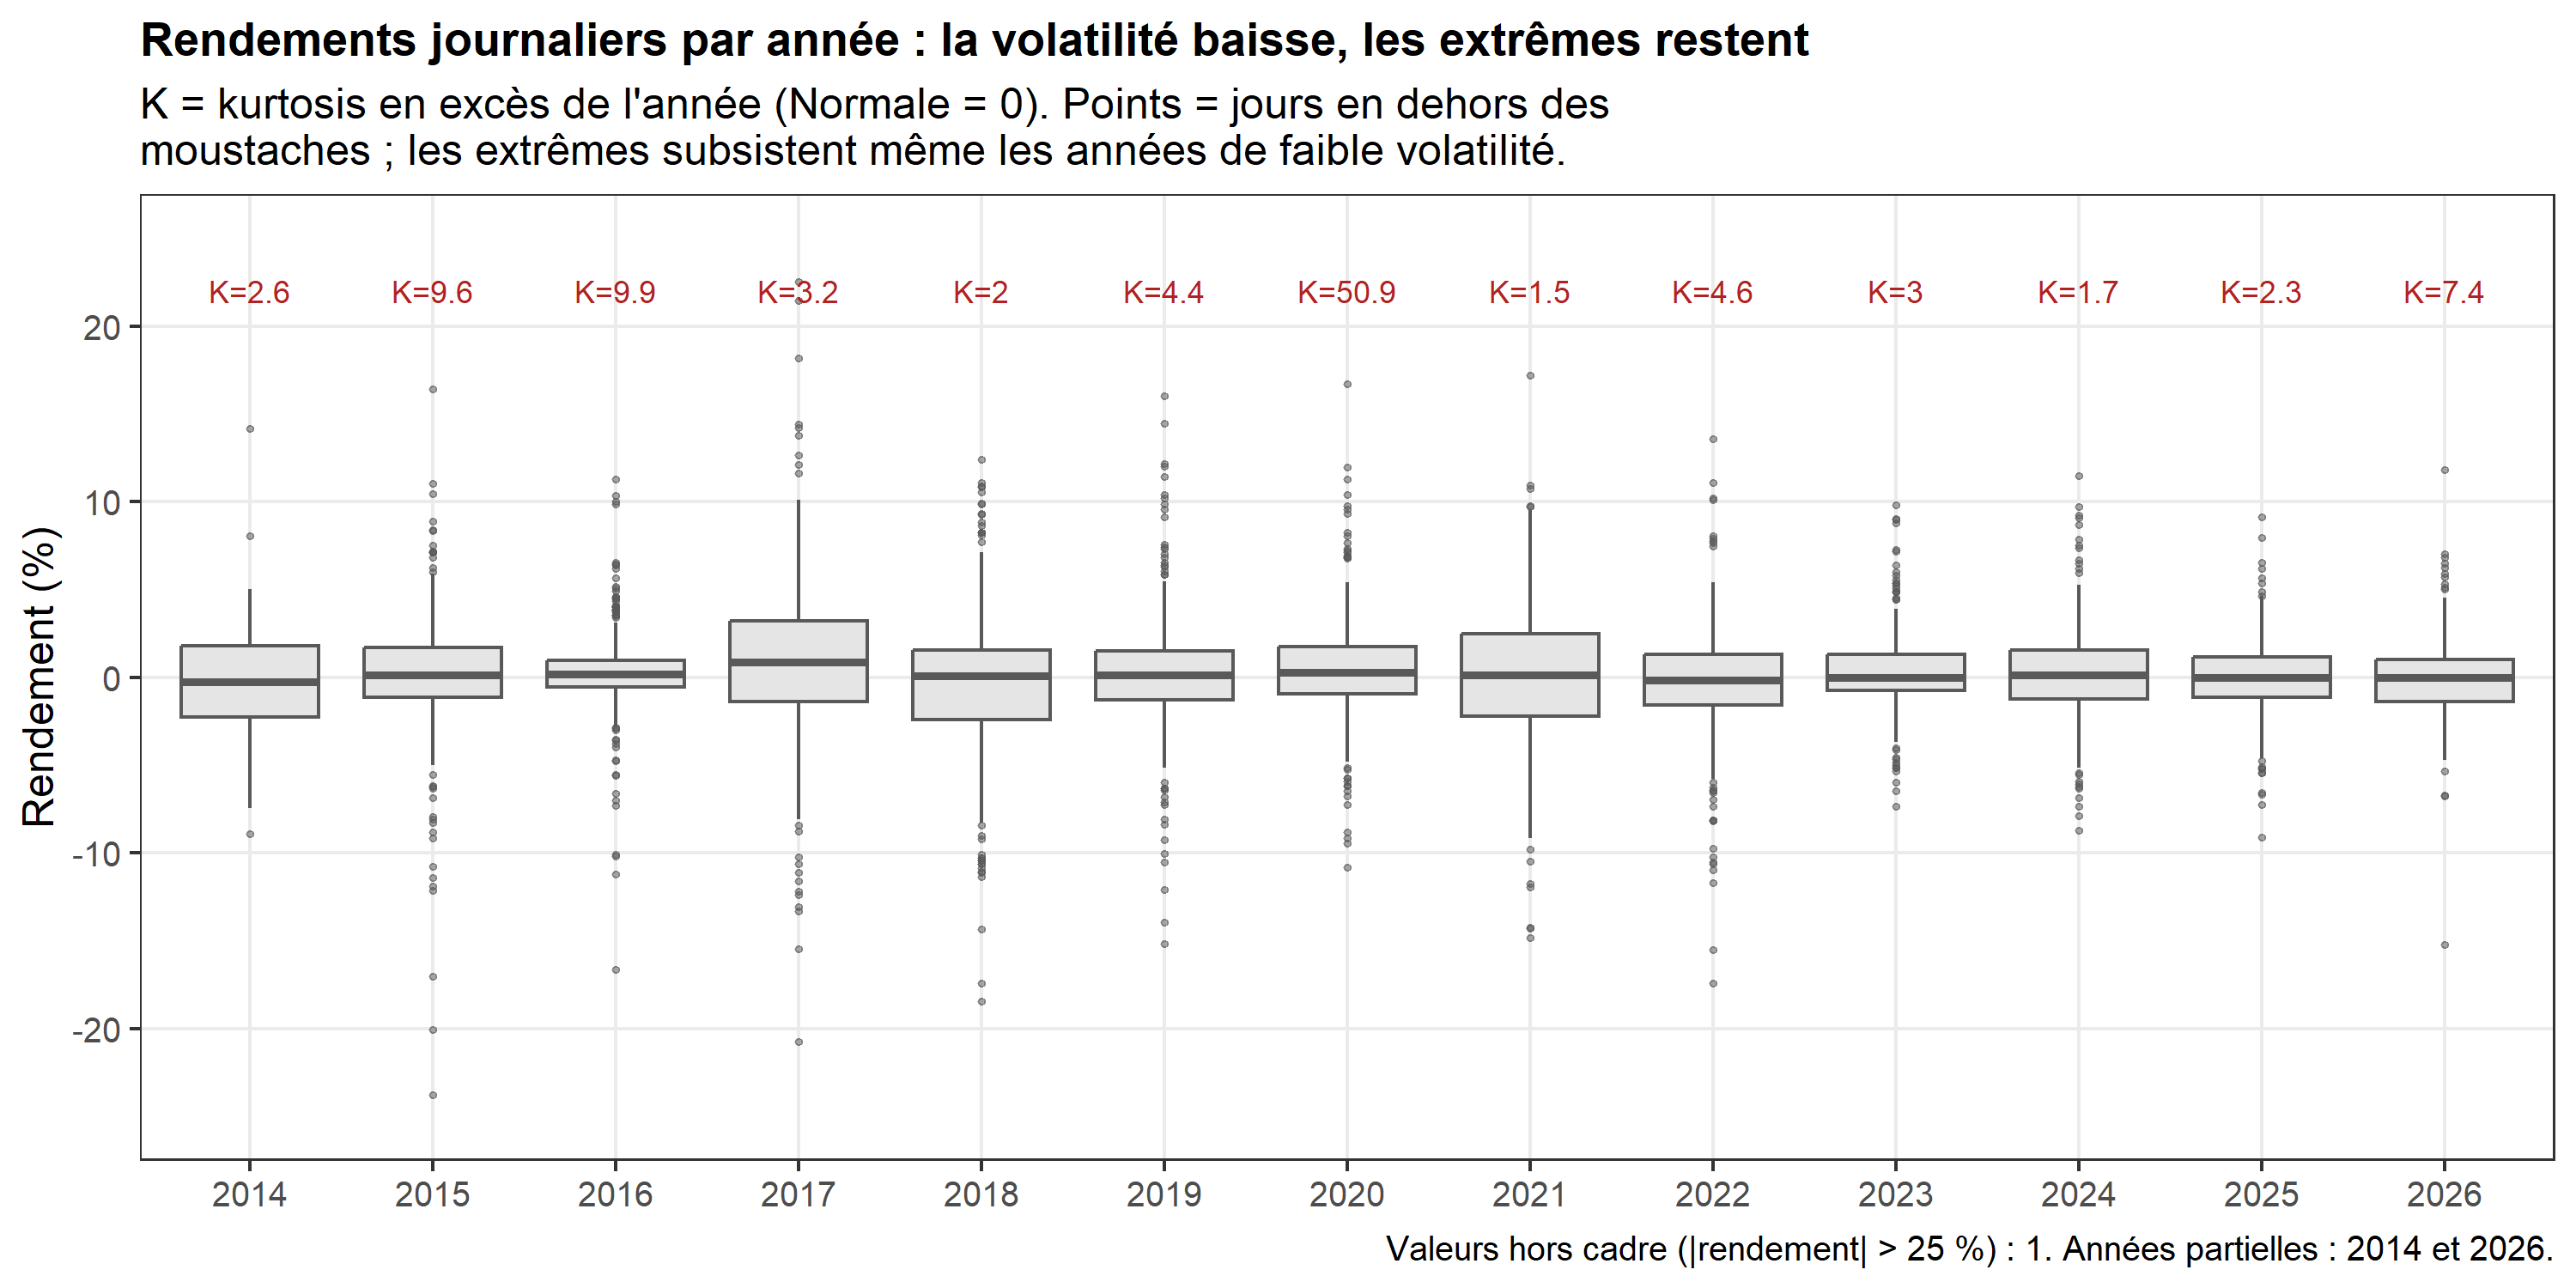
\includegraphics[width=1\linewidth]{D6_returns_by_year.png}
	\caption{Daily log returns by calendar year. $K$ is the excess kurtosis of the year (Normal $=0$); points are days outside the whiskers. Figure labels are in French. The dispersion falls over time, but extreme days remain in every year; the 2020 value ($K = 50.9$) is dominated by 2020-03-12.}
	\label{fig:returns-by-year}
\end{figure}

\begin{econbox}[Economic reading]
	Two properties of the data frame the rest of the paper. First, the market never closes: there is no pause to absorb information and no weekend gap, so a ``next day'' is the next calendar day, not the next trading day. Second, volatility is high by the standards of a currency (a daily standard deviation of $3.5\,\%$ over the sample, about $2.2$--$2.8\,\%$ since 2023). Table~\ref{tab:data-yearly} describes this decline; it does not explain it, and no cause is tested in this paper.
\end{econbox}

% ═════════════════════════════════════════════════════════════════
\section{Single-regime GARCH(1,1): Normal versus Student's $t$}
\label{sec:garch}
% ═════════════════════════════════════════════════════════════════

\subsection{Objective and specification}

This section estimates a GARCH(1,1) on the 4,394 daily log returns (scaled by 100, 2014-09-18 to 2026-09-28), compares Normal and Student's $t$ innovations, keeps the better specification, and documents its diagnostics and flags. No other specification is explored: the aim is to apply the pipeline built on EUR/USD, not to search for a better model of Bitcoin.

The model is
\begin{equation}
	r_t = \mu + \varepsilon_t, \qquad \varepsilon_t = \sigma_t z_t, \qquad
	\sigma_t^2 = \omega + \alpha\,\varepsilon_{t-1}^2 + \beta\,\sigma_{t-1}^2,
\end{equation}
where $z_t$ has zero mean and unit variance and is either standard Normal or a Student's $t$ rescaled to unit variance with $\nu$ degrees of freedom \citep{engle1982,bollerslev1986,bollerslev1987}. Estimation uses the Python package \texttt{arch}, by maximum likelihood.

The selection rule was fixed before any estimation on Bitcoin data: minimum BIC, with AIC reported; in case of disagreement both are documented and the BIC decides. Convergence is required. Residual diagnostics are Ljung--Box on $z_t^2$ (lags 10 and 20) and an ARCH-LM test on the \emph{standardised} residuals; a rejection at 5\,\% is documented as a limit, with no search for another specification. If $\hat\nu \le 4$, the theoretical kurtosis $6/(\nu-4)$ is infinite and is not compared with the empirical one.

\subsection{Results}

\begin{table}[H]
	\centering
	\caption{GARCH(1,1) on BTC-USD, Normal versus Student's $t$}
	\label{tab:garch-results}
	\small
	\begin{tabular}{lrr}
		\toprule
		& Normal & Student's $t$ \\
		\midrule
		$\mu$ (\%/day) & $0.1455$ ($p=0.001$) & $0.1113$ ($p=1.2\times10^{-4}$) \\
		$\omega$ & $0.4995$ ($p=5.5\times10^{-4}$) & $0.1906$ ($p=0.0146$) \\
		$\alpha$ & $0.1267$ ($p=2.6\times10^{-5}$) & $0.1074$ ($p=1.1\times10^{-14}$) \\
		$\beta$ & $0.8431$ ($p\approx 0$) & $0.8926$ ($p\approx 0$) \\
		$\nu$ (s.e.) & --- & $3.176$ ($0.122$) \\
		Log-likelihood & $-11{,}294.8$ & $-10{,}752.9$ \\
		AIC & $22{,}597.7$ & $\mathbf{21{,}515.8}$ \\
		BIC & $22{,}623.2$ & $\mathbf{21{,}547.7}$ \\
		Persistence $\alpha+\beta$ & $0.9697$ & $1.0000$ (boundary) \\
		Half-life (days) & $22.5$ & undefined \\
		Long-run $\sigma$ (\%/day) & $4.06$ & undefined \\
		Ljung--Box on $z^2$, lag 10 / 20 ($p$) & $0.895$ / $0.989$ & $0.914$ / $0.950$ \\
		ARCH-LM, 10 lags, standardised ($p$) & $0.895$ & $0.916$ \\
		Excess kurtosis of $z$ (empirical) & $11.56$ & $12.83$ \\
		Theoretical kurtosis $6/(\nu-4)$ & --- & infinite ($\nu\le 4$) \\
		\bottomrule
	\end{tabular}
\end{table}

Both models converge. The Student's $t$ is retained: AIC and BIC agree, with $\Delta$AIC $\approx 1{,}082$ and $\Delta$BIC $\approx 1{,}076$ in its favour. On EUR/USD the same differences were about $162$ and $155$ in the companion EUR/USD paper \citep{ZEWU2026fx}: the gap is nearly seven times larger here, consistent with much heavier tails.

\begin{figure}[H]
	\centering
	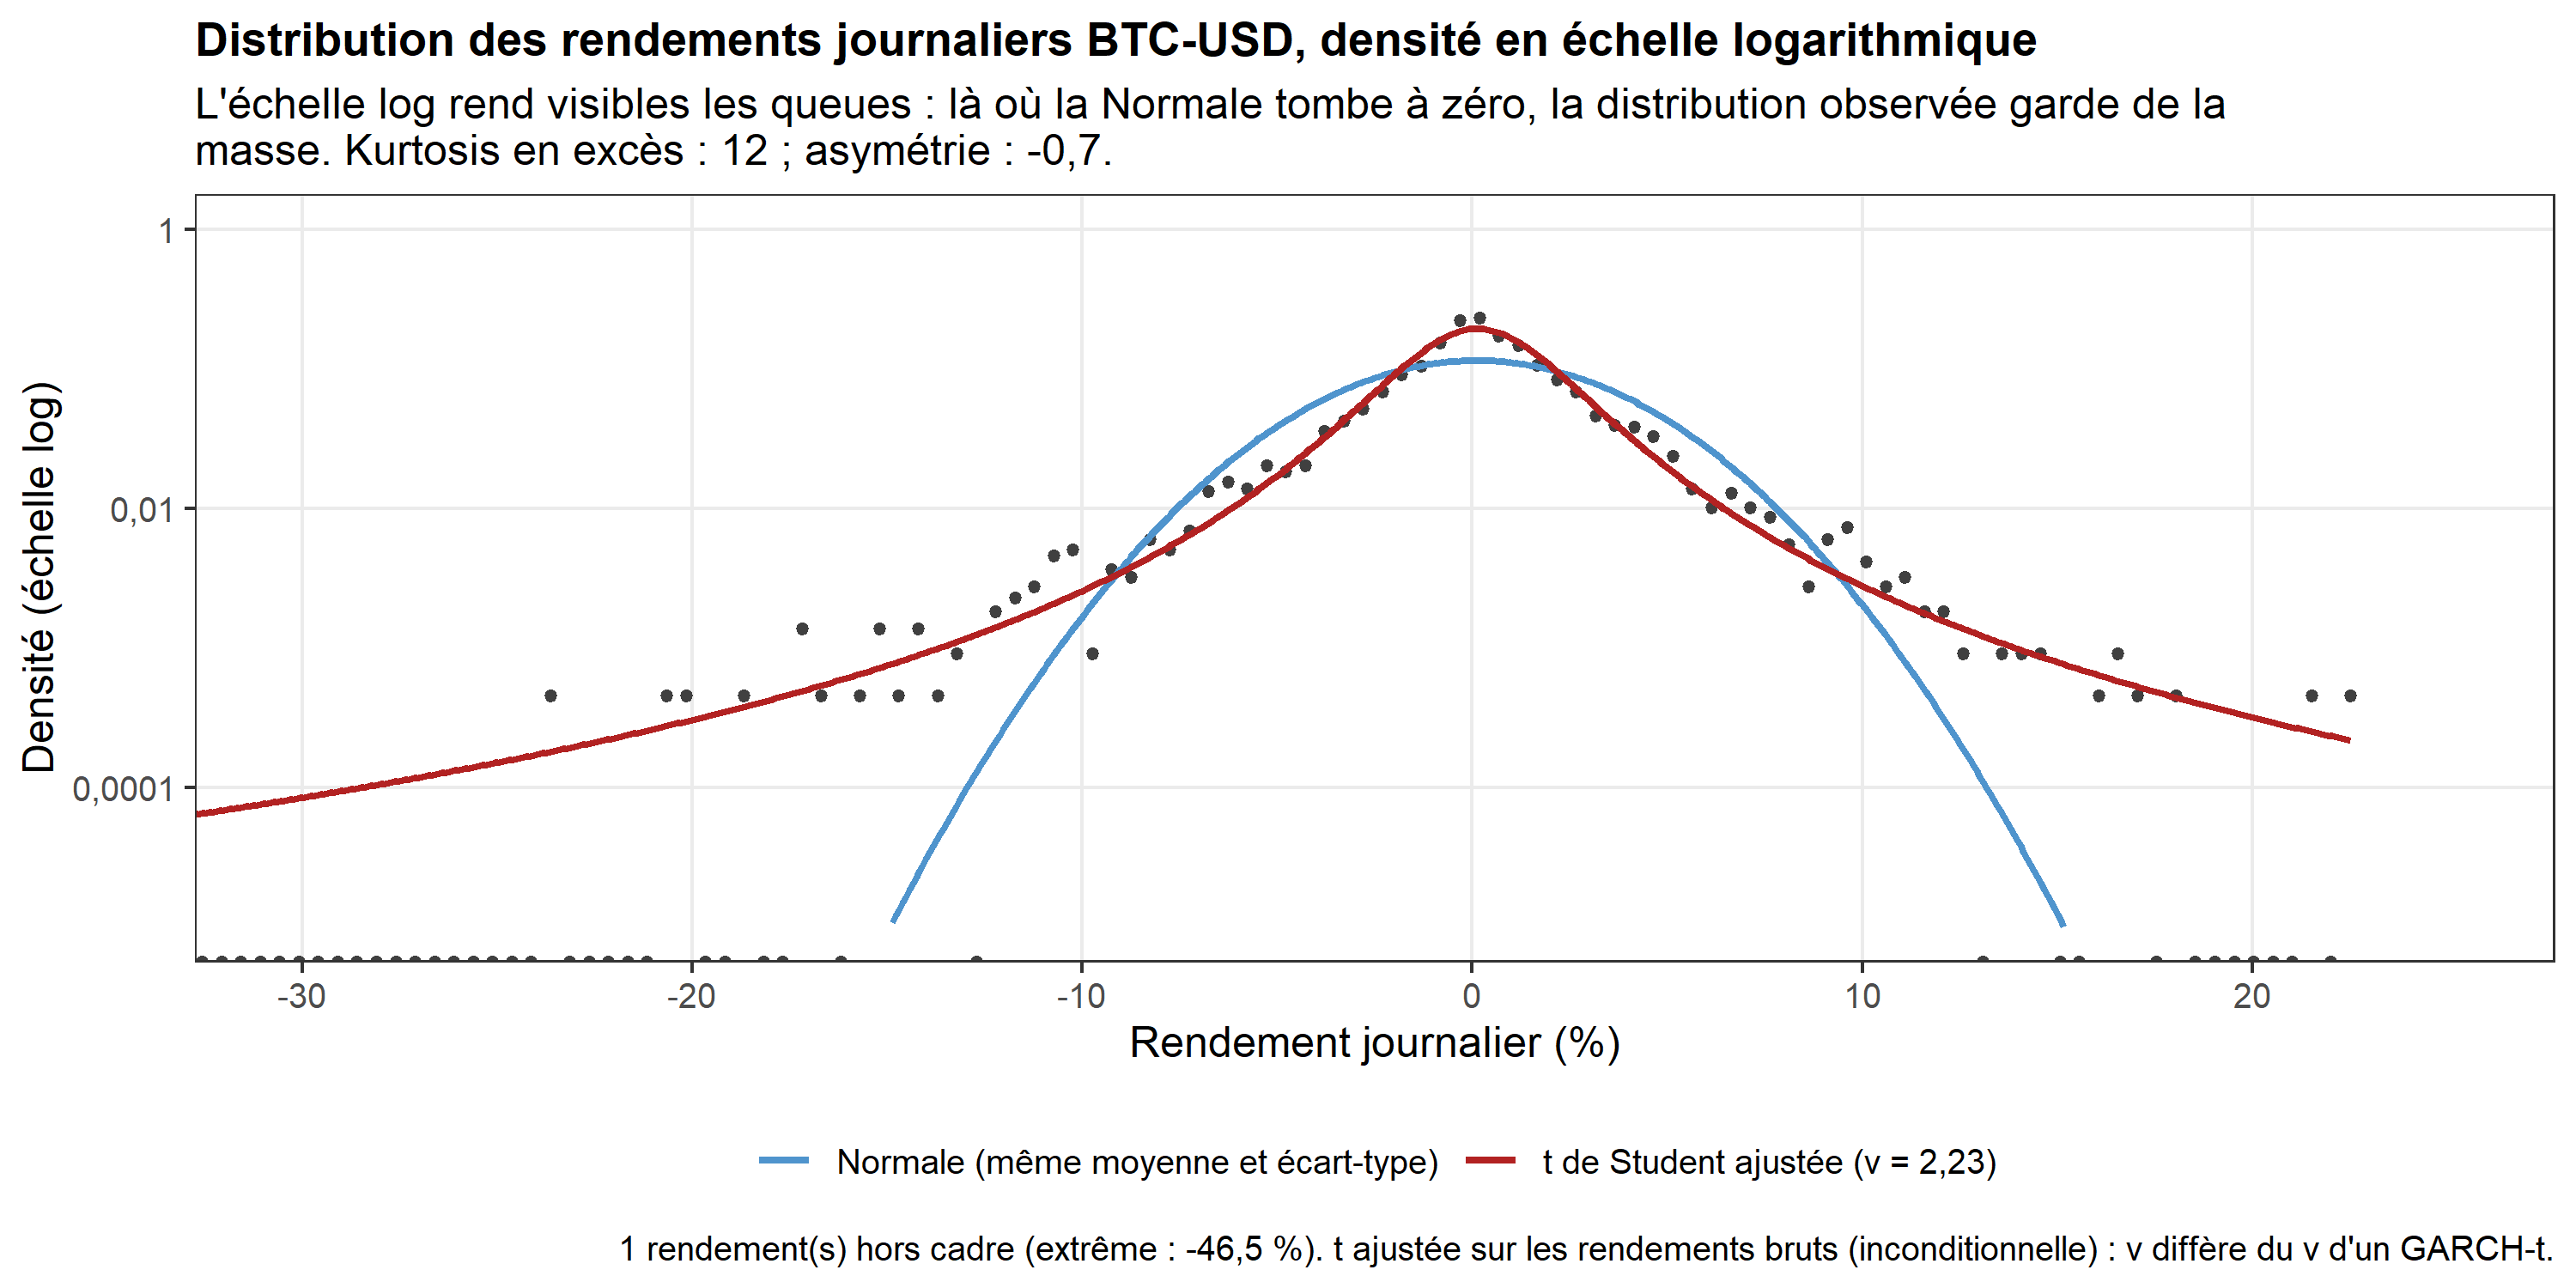
\includegraphics[width=1\linewidth]{D1_histogram_log_density.png}
	\caption{Distribution of daily BTC-USD log returns, density on a log scale. Where the Normal falls to zero, the observed distribution keeps mass. The fitted $t$ is estimated on the raw returns (unconditional, $\nu=2.23$) and is not the conditional $\nu = 3.18$ of the GARCH. One return ($-46.5\,\%$) lies outside the frame. Figure labels are in French.}
	\label{fig:density}
\end{figure}

\subsection{Persistence at the boundary}
\label{sec:garch-igarch}

Under the Student's $t$, $\hat\alpha + \hat\beta = 0.107385 + 0.892615 = 1.000000$. The optimiser of \texttt{arch} imposes $\alpha+\beta \le 1$, so the constrained maximum sits on the bound, which suggests that the unconstrained likelihood would peak beyond it. Three consequences:
\begin{itemize}
	\item The half-life ($\approx 8\times10^{10}$ days) and the long-run standard deviation ($\approx 148{,}000\,\%$) that the script prints are numerical artefacts: the unconditional variance is not defined when $\alpha+\beta=1$. \textbf{They must not be reported}, and they are not.
	\item The standard errors of $\alpha$ and $\beta$ rely on asymptotic normality, which does not hold at a boundary; they are to be read with caution.
	\item $\omega$ ($p=0.015$) no longer has a long-run-level interpretation.
\end{itemize}

\begin{econbox}[Economic interpretation of persistence]
	Under the Normal, a volatility shock loses half its intensity in about 22 days; under the $t$, there is no reversion to a mean level (IGARCH behaviour). As on EUR/USD, where persistence moved from $0.9945$ to $0.9985$ with the distribution, the persistence depends on the distributional assumption --- here far more strongly. No single half-life is therefore reported. A reading of the $t$ result as ``Bitcoin has no normal level of risk'' would fit an asset with no institutional anchor, but a persistence of one is also the classical symptom of unmodelled structural breaks \citep{lamoureuxlastrapes1990}; this section does not separate the two readings (see sections~\ref{sec:msgarch} and~\ref{sec:era}).
\end{econbox}

\subsection{A tail parameter of 3.18: infinite kurtosis and the reliability of the tests}

With $\hat\nu = 3.18 \le 4$, the fourth moment of the innovation is infinite. Two things follow.

First, the empirical kurtosis of the standardised residuals (12.83) converges to no value: it cannot serve as a measure of fit, and the check of comparing it with $6/(\nu-4)$ is inapplicable.

Second, the Ljung--Box and ARCH-LM tests on $z_t^2$ assume that $z_t^2$ has a finite variance, which is false when $E[z^4]$ is infinite. The $p$-values above 0.9 in Table~\ref{tab:garch-results} are therefore \emph{weak} evidence of no residual ARCH, not strong evidence.

For that reason a complementary test was run on $|z_t|$, which has a finite variance even when $\nu \le 4$, so that Ljung--Box remains valid. It was added \emph{after} the fact, for a known theoretical reason, and was not part of the pre-specified diagnostics.

\begin{table}[H]
	\centering
	\caption{Ljung--Box test on $|z_t|$ (Student's $t$ model; added after the fact)}
	\label{tab:garch-absz}
	\begin{tabular}{lrr}
		\toprule
		Lag & Statistic & $p$-value \\
		\midrule
		10 & $22.03$ & $0.0150$ \\
		20 & $38.27$ & $0.0082$ \\
		\bottomrule
	\end{tabular}
\end{table}

\begin{limitbox}
	\textbf{Residual dependence is detected where the tests on $z^2$ saw nothing.} The single-regime $t$ GARCH does not capture all the dynamics of volatility, and the absence of rejection on $z_t^2$ reflected a lack of power, not a good fit. The conclusion ``no residual ARCH'' is withdrawn. As the selection rule requires, the rejection is documented as a limit, without exploring other specifications. The result is compatible with a change of volatility level or regime (section~\ref{sec:msgarch}), but does not demonstrate it: asymmetry or long memory would produce the same signal. The $p$-values are not corrected for the estimation of the parameters.
\end{limitbox}

\subsection{The largest shock and the shape of the tails}

\begin{figure}[H]
	\centering
	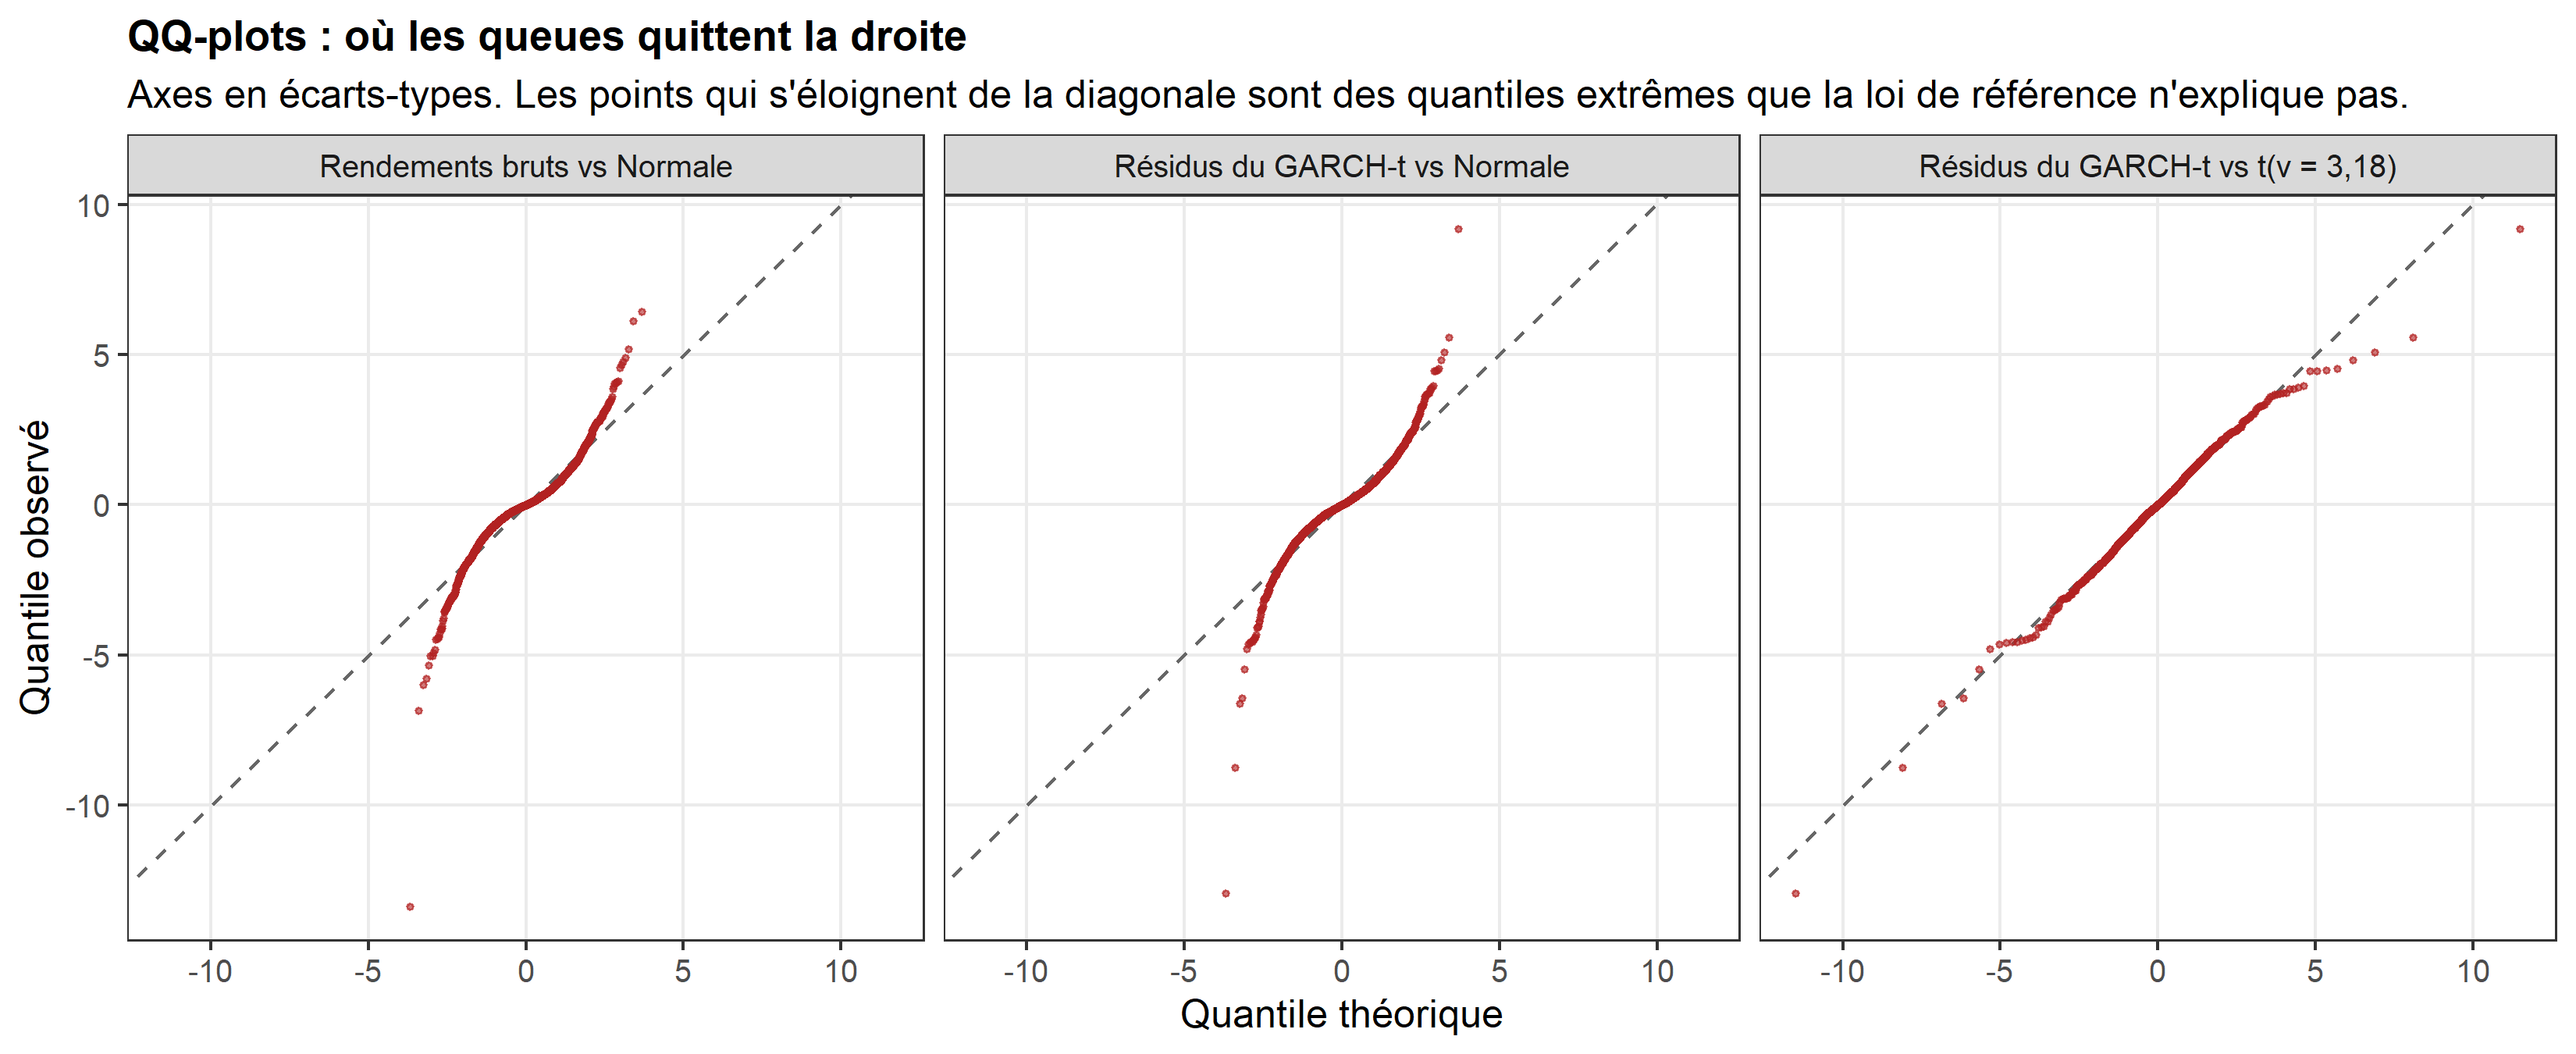
\includegraphics[width=1\linewidth]{D2_qqplots.png}
	\caption{QQ-plots in standard-deviation units: raw returns against the Normal, GARCH-$t$ standardised residuals against the Normal, and the same residuals against the $t$ ($\nu=3.18$). Points that leave the diagonal are extreme quantiles that the reference law does not explain. Figure labels are in French.}
	\label{fig:qq}
\end{figure}

The Normal is clearly rejected as a description of the tails: in the first two panels the extreme quantiles leave the diagonal sharply. The standardised residuals of the $t$ model follow the $t$ closely over most of the range. In the third panel the largest upper quantiles lie below the diagonal; with so few points this is not interpreted.

The worst standardised shock of the $t$ model is $-12.92$, on 2020-03-12. The probability of a shock this large or larger on that side is $1.84\times10^{-38}$ under the Normal --- an event with no meaning on the scale of the age of the universe --- and $7.86\times10^{-5}$ under the $t$, about one day in 12,700, or roughly 35 years. Over 4,394 observations, about $0.35$ such events are expected under the $t$; one is observed.

\subsection{The mean}

The estimated mean is significant ($\hat\mu = 0.11\,\%$ per day, $p = 1.2\times10^{-4}$), whereas on EUR/USD it was not. This is \emph{not} a sign of inefficiency or predictability. It is the realised drift of an asset that went from about \$457 to more than \$83,000 over the sample, with the selection bias that comes from studying Bitcoin ex post. The consequence for the design (the mean of the price range) is handled in section~\ref{sec:price-range}.

\subsection{A hypothesis to test, not a conclusion}

Level breaks in the unconditional variance push the estimated persistence towards one and inflate the tails of a single-regime GARCH \citep{lamoureuxlastrapes1990}. The yearly profile of Table~\ref{tab:data-yearly} is compatible with this but does not prove it. A \textbf{falsifiable prediction} was fixed before the next step: if the ``era'' explanation is right, separate estimations before and after the cut of 2020-09-22 should give a persistence clearly below one and a $\nu$ above $3.18$ in both halves. If not, the hypothesis loses support. Since a median cut has low power, a failure to confirm would not invalidate it definitively either. The Markov-switching model (section~\ref{sec:msgarch}) is the main test; the result of the split-sample test is in section~\ref{sec:era}.

\subsection{Limits of this step}

\begin{itemize}
	\item The specification (Normal against $t$) was chosen on the full sample. The choice is massive ($\Delta$BIC $\approx 1{,}076$), hence little sensitive to hindsight; the parameters used in the backtest are re-estimated on an expanding window.
	\item The tests on $z^2$ have low power (infinite fourth moment); the test on $|z|$ rejects.
	\item The GARCH has a single regime: the persistence and $\nu$ results are to be read in the light of section~\ref{sec:msgarch}.
\end{itemize}


% ═════════════════════════════════════════════════════════════════
\section{Markov-Switching GARCH ($K=2$)}
\label{sec:msgarch}
% ═════════════════════════════════════════════════════════════════

\subsection{Objective and specification}

This section applies, unchanged, the two-regime Markov-switching GARCH of the EUR/USD paper \citep{ZEWU2026fx} --- the specification of \citet{haasmittnikpaolella2004}, estimated with the R package \texttt{MSGARCH} \citep{ardia2019} --- to the Bitcoin returns. Two questions: does the pipeline run and produce interpretable diagnostics, and what does the frozen ``regime or era'' rule (section~\ref{sec:era}) give on these data?

Each of the two regimes $k\in\{1,2\}$ has its own GARCH(1,1) variance with Student's $t$ innovations,
\begin{equation}
	r_t = \sigma_{k,t}\, z_t, \qquad \sigma_{k,t}^2 = \omega_k + \alpha_k\, r_{t-1}^2 + \beta_k\, \sigma_{k,t-1}^2,
\end{equation}
and the regime follows a Markov chain with transition matrix $P$ (option \texttt{do.mix = FALSE}). As on EUR/USD, no mean equation is estimated: returns are treated as having zero mean, which is the usual \texttt{MSGARCH} convention. Regime-switching GARCH models are an established family \citep{hamiltonsusmel1994,gray1996}, whose forecasting performance has been studied on large panels \citep{ardia2018}.

The ``volatile'' regime is defined \emph{before} looking at results as the one whose dominant days (smoothed probability above 0.5) have the highest realised standard deviation. The long-run $\sigma$, $\omega/(1-\alpha-\beta)$, is not used: it is unreliable near the IGARCH boundary.

\begin{table}[H]
	\centering
	\small
	\caption{Declared differences with the EUR/USD implementation}
	\label{tab:ms-diffs}
	\begin{tabular}{cp{4.2cm}p{7cm}}
		\toprule
		& Difference & Reason \\
		\midrule
		D1 & Returns in \% ($\times 100$) & Consistency with section~\ref{sec:garch}; better-conditioned optimisation. $\alpha$, $\beta$, $\nu$ and $P$ are scale-invariant. \\
		D2 & Single-regime $t$ GARCH estimated \emph{inside} \texttt{MSGARCH} (zero mean) & Compare $K=1$ and $K=2$ with identical mean specifications. \\
		D3 & ``Regime or era'' rule applied mechanically by the script & No reading of the result by eye. \\
		D4 & Filtered probabilities and Viterbi path exported & Needed for the real-time use of the regime probabilities (section~\ref{sec:backtest}). \\
		D5 & Multiple restarts; the best optimum becomes the final fit & See section~\ref{sec:ms-optimum}. \\
		D6 & Verdicts \texttt{ERA}, \texttt{NOT\_\allowbreak{}ERA}, \texttt{NO\_\allowbreak{}VOLATILE\_\allowbreak{}DAY} & ``Regime'' suggested that a regime had been found. \\
		D7 & ``Persistent regime'' starts and logit noise on the transition probabilities & The default start and its neighbourhood reach only micro-regime optima (section~\ref{sec:ms-optimum}). \\
		\bottomrule
	\end{tabular}
\end{table}

\subsection{Finding the optimum: sensitivity to the starting point}
\label{sec:ms-optimum}

The likelihood of a regime-switching model has several local optima, so the estimation uses \textbf{21 starting points}: the default point of \texttt{MSGARCH}, 8 perturbed points and 12 ``persistent regime'' points (transition probabilities close to one). The 21 fits fall as follows: 10 on the persistent optimum (nine at $-10{,}708.78$, one at $-10{,}708.94$); 5 on a micro-regime optimum at $-10{,}713.36$ (one of them from a persistent start); 4 at $-10{,}714.83$; the default point ($-10{,}716.45$); and one isolated fit ($-10{,}737.17$).

The best optimum is reproduced 10 times, \emph{all} from persistent starts (10 of the 12 persistent starts, none of the 8 perturbed ones). Neither the default starting point of \texttt{MSGARCH} nor its neighbourhood reaches it. The consequence for the reading is large: the micro-regime optima give expected durations of 2 to 6 days and 91\,\% of ambiguous days, while the persistent optimum gives 73 and 36 days. With the same number of parameters, the persistent solution gains 4.58 log-likelihood points, i.e.\ $\Delta$AIC $=\Delta$BIC $=-9.2$. Global optimality is not demonstrated, only supported by this repetition.

\begin{figure}[H]
	\centering
	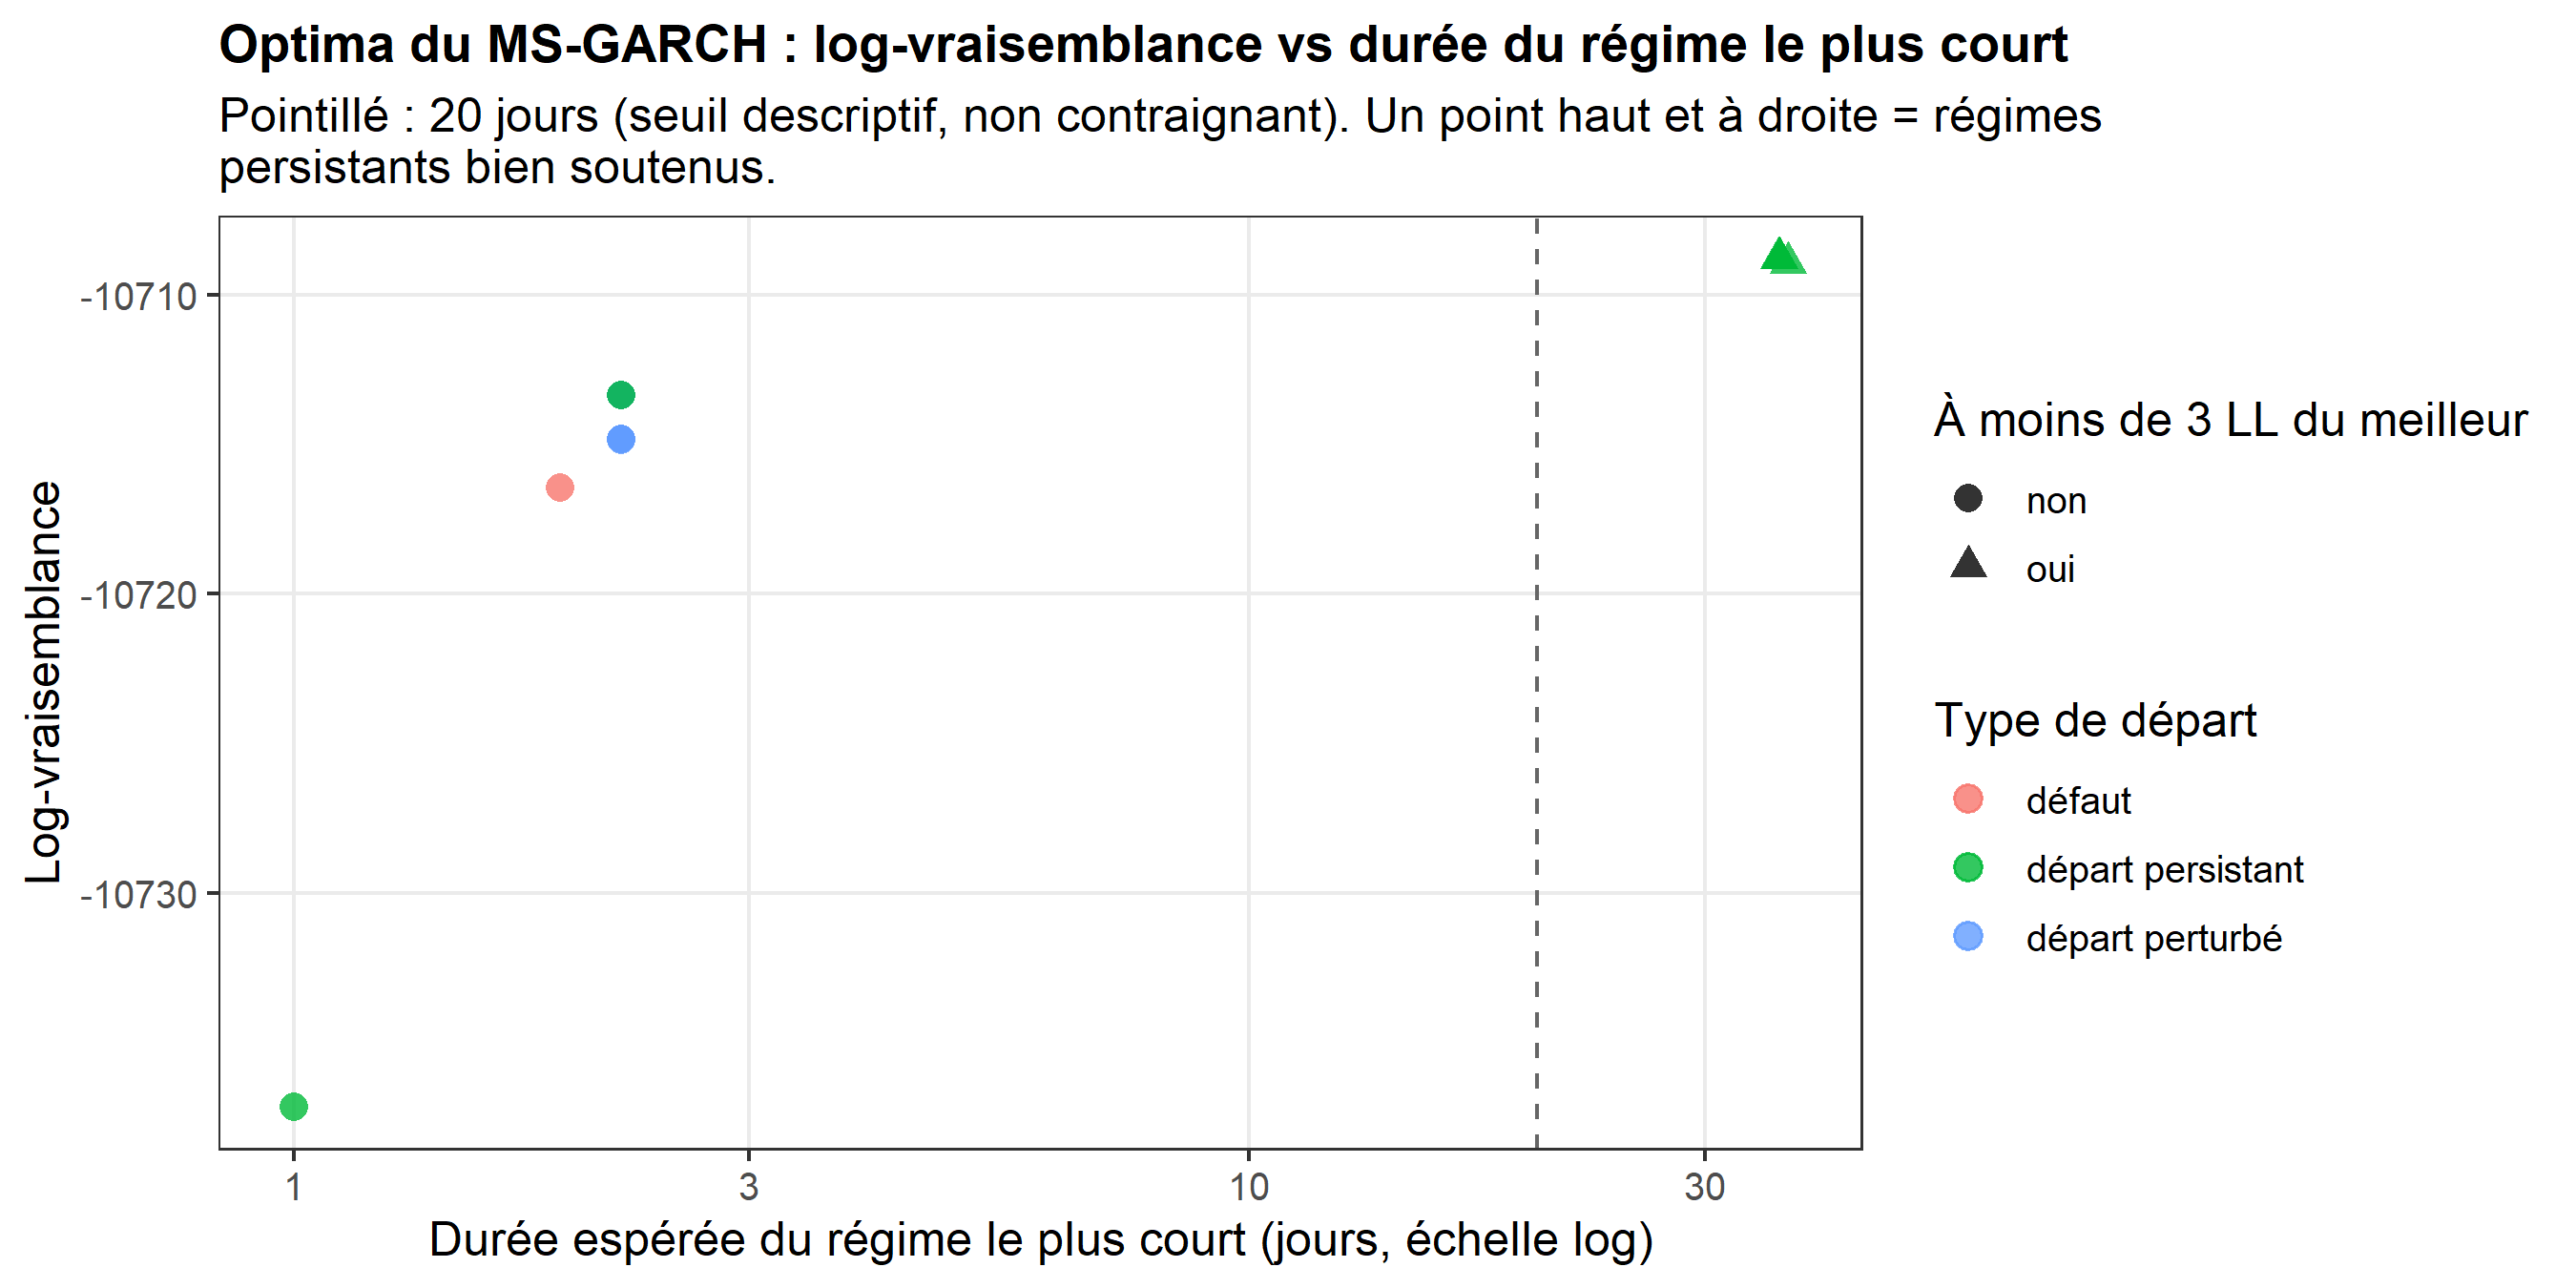
\includegraphics[width=0.95\linewidth]{08_optima_ll_vs_duration.png}
	\caption{The optima of the MS-GARCH: log-likelihood against the expected duration of the shortest regime (log scale). Two clear basins: micro-regimes ($\approx 2$ days) and persistent regimes ($\approx 36$ days), with no intermediate solution. Legend: \texttt{default} = default starting point; \texttt{pert} = perturbed starts; \texttt{pers} = ``persistent regime'' starts. Figure labels are in French.}
	\label{fig:ms-optima}
\end{figure}

\subsection{Results}

\begin{table}[H]
	\centering
	\caption{MS-GARCH ($K=2$) on BTC-USD: final fit (standard errors in parentheses)}
	\label{tab:ms-params}
	\begin{tabular}{lrr}
		\toprule
		& Volatile regime & Calm regime \\
		\midrule
		$\omega$ & $0.3780$ ($0.131$) & $0.1784$ ($0.140$) \\
		$\alpha$ & $0.0835$ ($0.058$) & $0.0750$ ($0.106$) \\
		$\beta$ & $0.9044$ ($0.0084$) & $0.9240$ ($0.0013$) \\
		$\nu$ & $3.95$ ($0.39$) & $2.30$ ($0.068$) \\
		Persistence $\alpha+\beta$ & $0.988$ & $0.99900$ \\
		Half-life within regime & 57 days & $\approx 695$ days (unreliable) \\
		Realised $\sigma$ on dominant days (\%/day) & $3.81$ & $2.61$ \\
		Expected duration $1/(1-P_{kk})$ & 72.8 days & 35.9 days \\
		Stationary probability & 67\,\% & 33\,\% \\
		\bottomrule
	\end{tabular}
\end{table}

The transition probabilities are $P(\text{volatile}\to\text{volatile}) = 0.9863$ and $P(\text{calm}\to\text{calm}) = 0.9722$. The log-likelihood is $-10{,}708.78$, AIC $21{,}437.56$, BIC $21{,}501.44$ (10 free parameters).

\textbf{Reading the $p$-values.} The \texttt{Pr(>|t|)} column printed by \texttt{MSGARCH} is one-sided; the two-sided $p$-value is twice the displayed value, and the values quoted here are two-sided. $\omega$ of the volatile regime has $p\approx 0.004$ and its $\alpha$ $p\approx 0.15$; $\omega$ and $\alpha$ of the calm regime ($p\approx 0.20$ and $0.48$) are not significant; $\beta$ and $\nu$ have $p\approx 0$.

\begin{figure}[H]
	\centering
	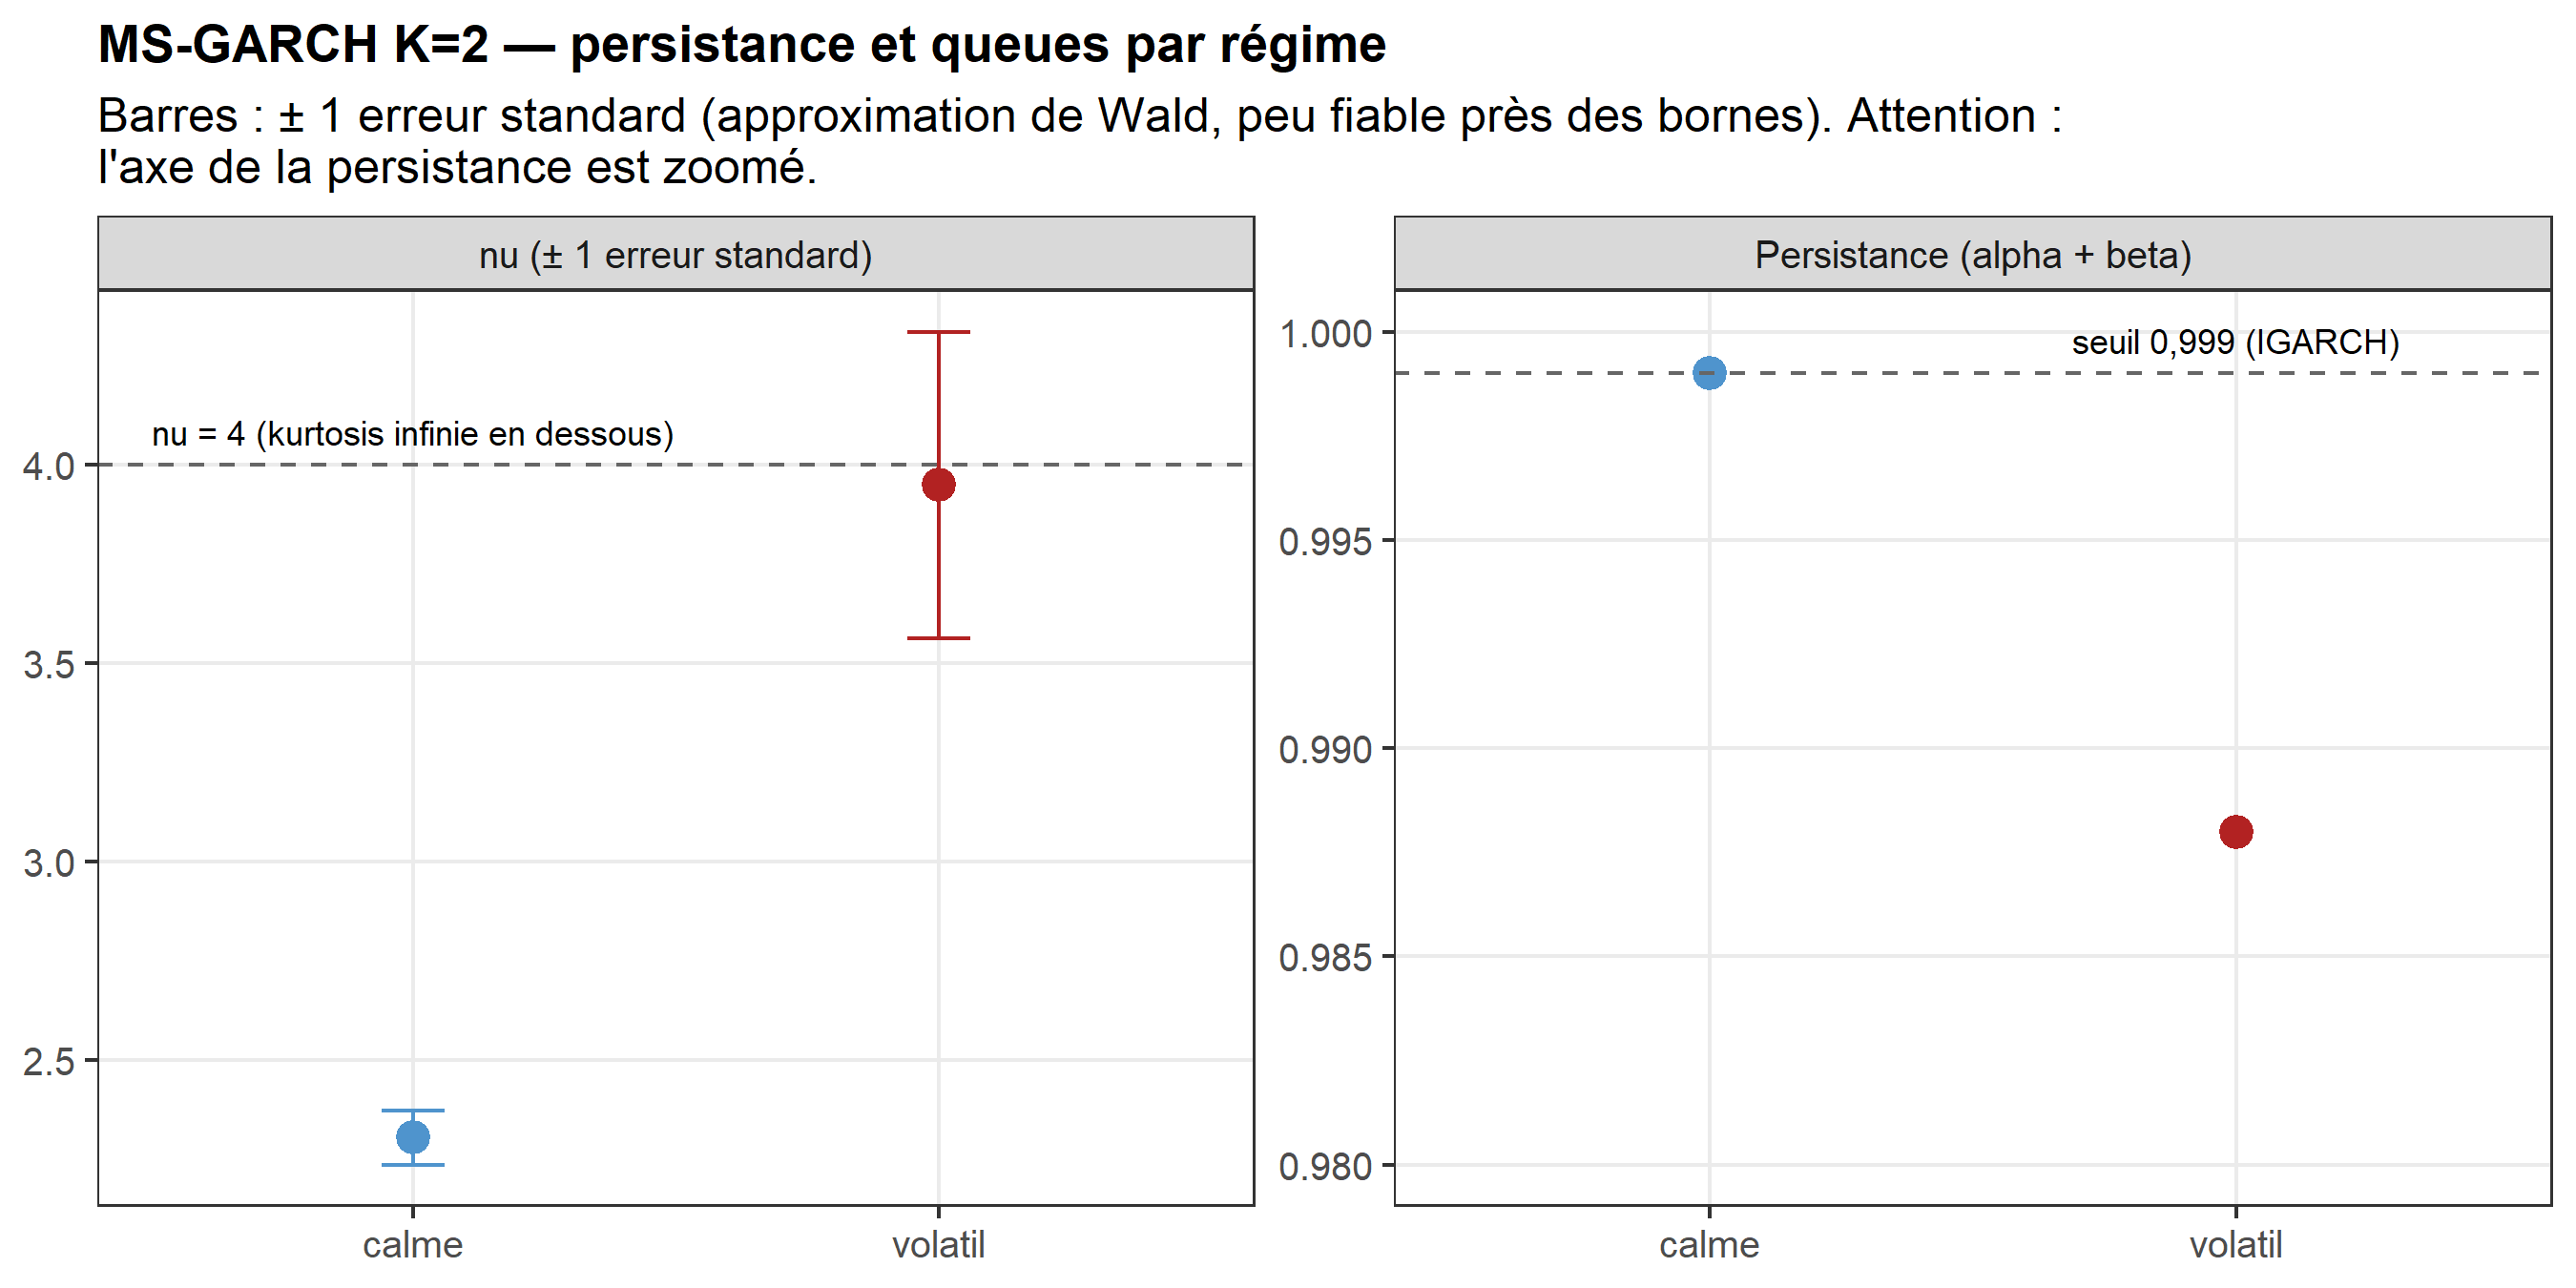
\includegraphics[width=1\linewidth]{03_params_by_regime.png}
	\caption{Tail parameter $\nu$ and persistence $\alpha+\beta$ by regime. Bars are $\pm 1$ standard error (a Wald approximation, unreliable near the bounds); the persistence axis is zoomed. Figure labels are in French.}
	\label{fig:ms-params}
\end{figure}

\subsection{Identification of the regimes}

The volatile regime occupies about 69\,\% of the days (label at 0.5) and the calm regime about 31\,\%. There are 26 volatile blocks and 51 switches over 4,394 days.

\begin{table}[H]
	\centering
	\small
	\caption{Longest blocks of each regime (smoothed probability above or below 0.5)}
	\label{tab:ms-blocks}
	\begin{tabular}{lrlr}
		\toprule
		Volatile block & Days & Calm block & Days \\
		\midrule
		2020-10-03 to 2022-08-09 & 676 & 2023-06-23 to 2023-11-07 & 138 \\
		2017-04-21 to 2018-09-08 & 506 & 2015-12-16 to 2016-04-18 & 125 \\
		2024-06-16 to 2025-04-12 & 301 & 2016-07-09 to 2016-10-24 & 108 \\
		2014-09-18 to 2015-05-08 & 233 & 2025-04-13 to 2025-07-29 & 108 \\
		\bottomrule
	\end{tabular}
\end{table}

\begin{figure}[H]
	\centering
	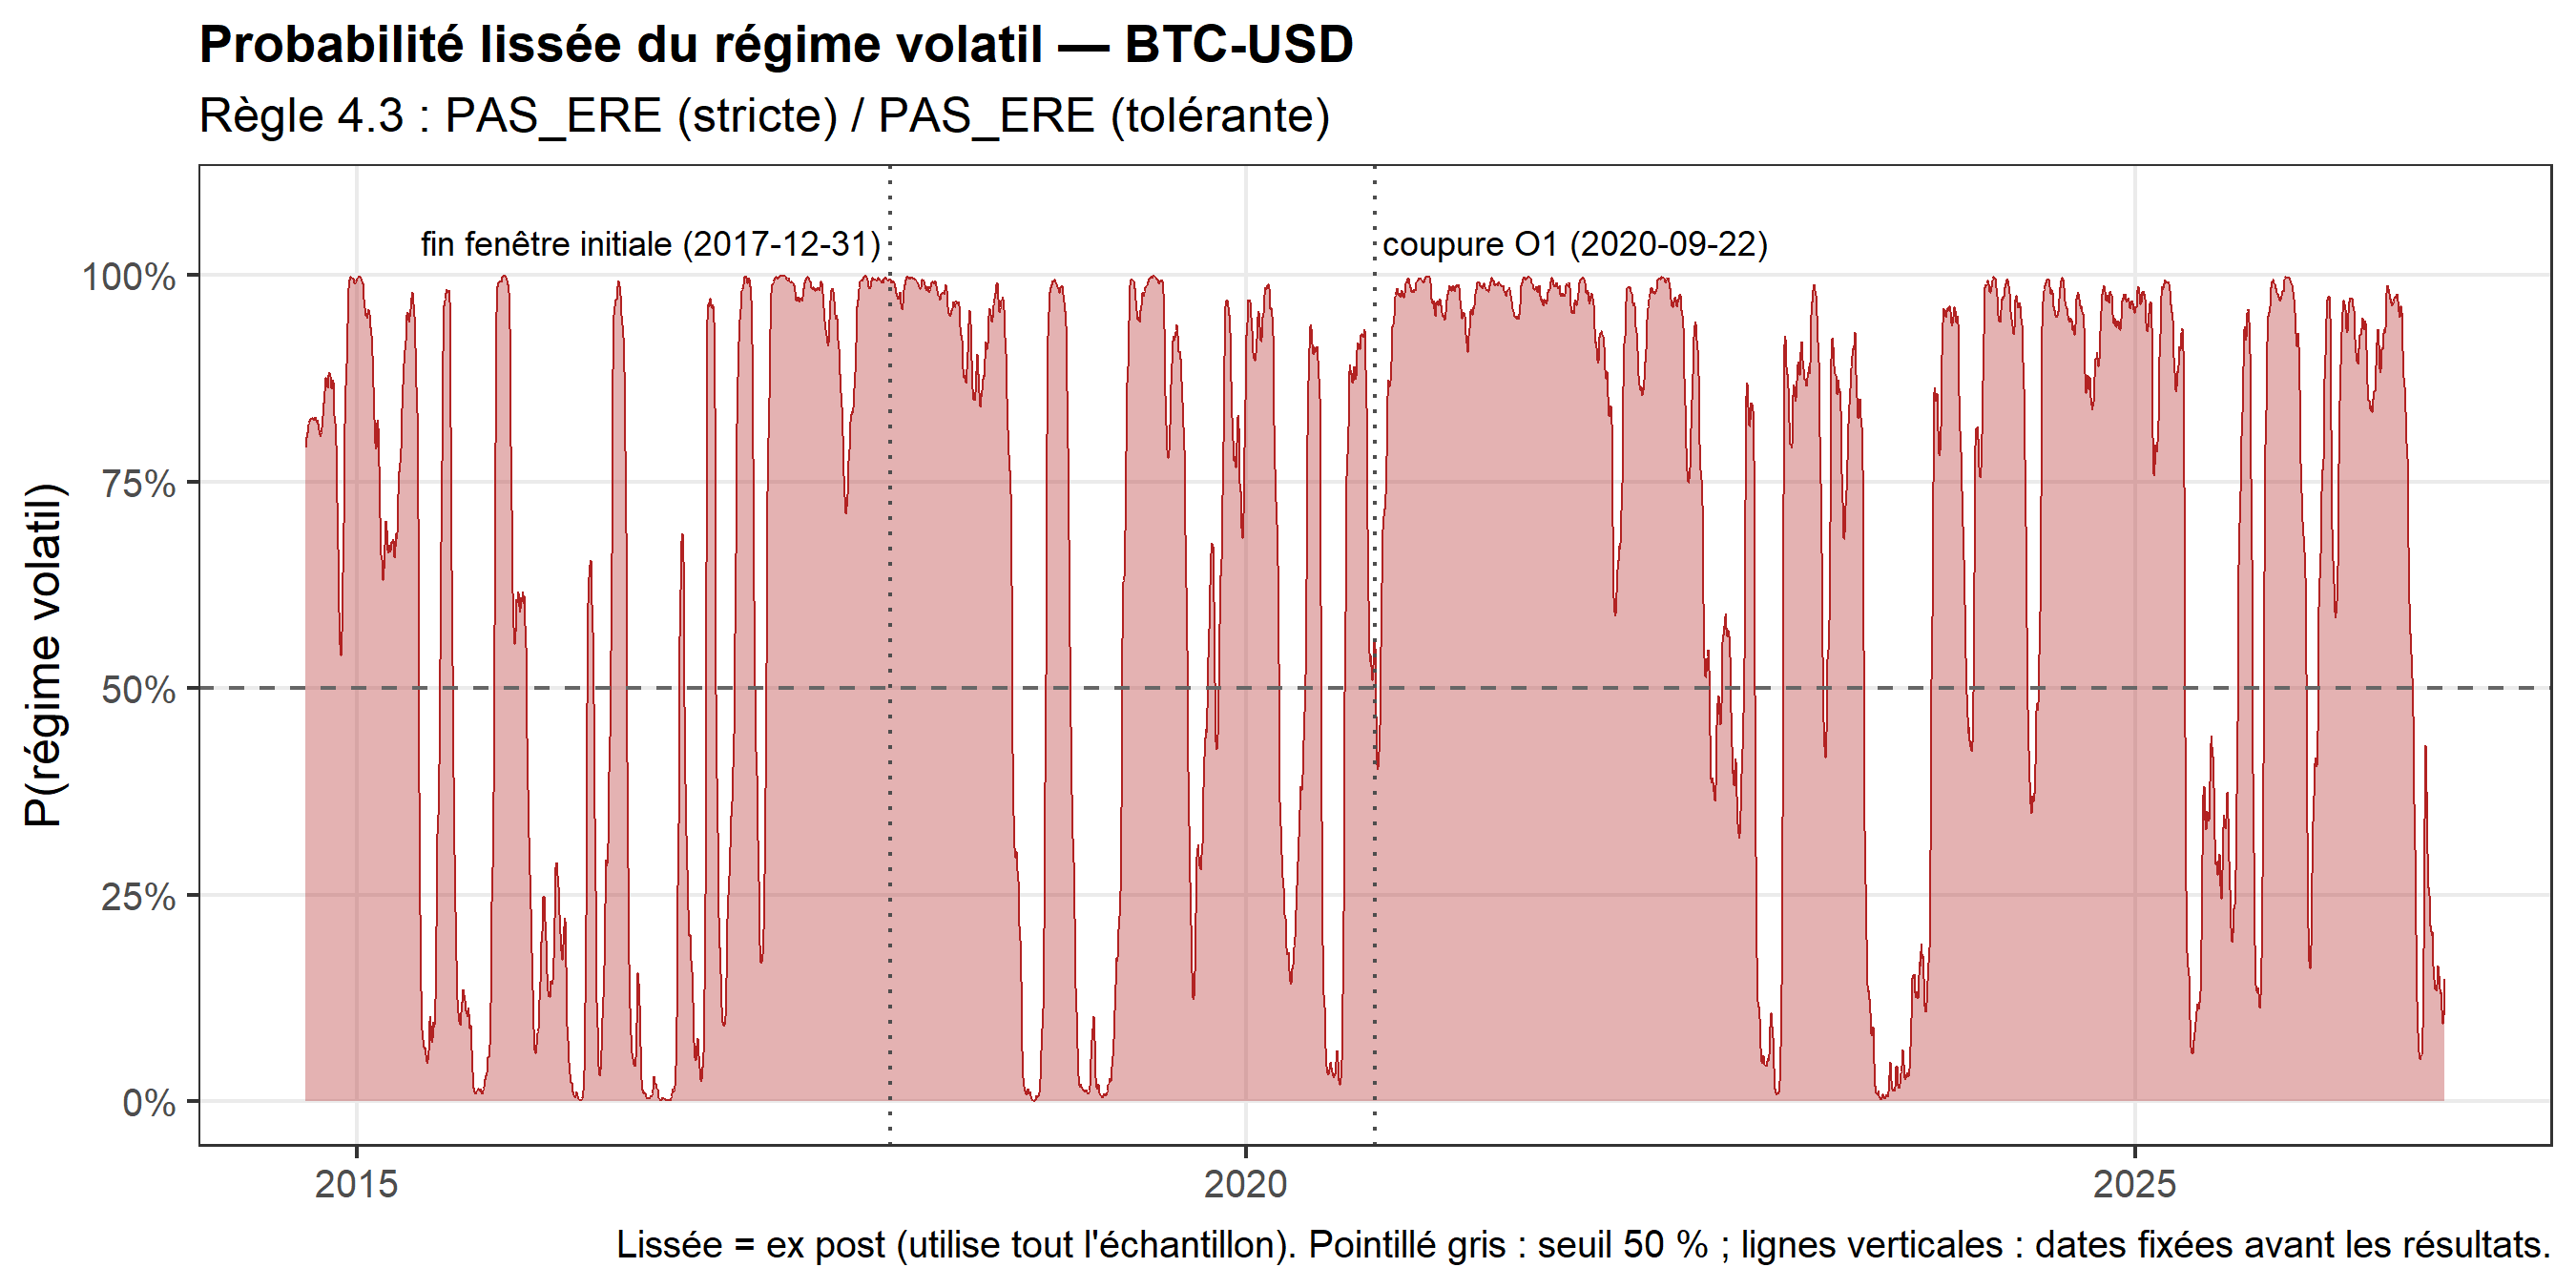
\includegraphics[width=1\linewidth]{01_smoothed_prob_highvol_fullsample.png}
	\caption{Smoothed probability of the volatile regime, full sample. The regimes alternate over the whole period; there is no single step. ``Smoothed'' means \emph{ex post}: it uses the whole sample. Figure labels are in French.}
	\label{fig:ms-smoothed}
\end{figure}

\textbf{The identification is imperfect}: 42.6\,\% of the days have a maximal smoothed probability below 0.9 (against 90.7\,\% at the micro-regime optimum). The durations are also very uncertain: the standard error of $P(\text{volatile}\to\text{volatile})$ is $0.0108$ for an exit probability of $0.0137$, so the duration of 72.8 days could be anything from several weeks to several months or more; a Wald interval is not reliable this close to the bound.

\subsection{Comparison with the single-regime GARCH}

\begin{table}[H]
	\centering
	\caption{$K=1$ versus $K=2$ (same scale, zero mean, both estimated in \texttt{MSGARCH})}
	\label{tab:ms-ic}
	\begin{tabular}{lrr}
		\toprule
		& $K=1$ & $K=2$ \\
		\midrule
		Free parameters & 4 & 10 \\
		Log-likelihood & $-10{,}755.49$ & $-10{,}708.78$ ($+46.71$) \\
		AIC & $21{,}518.99$ & $\mathbf{21{,}437.56}$ ($-81.4$) \\
		BIC & $21{,}544.54$ & $\mathbf{21{,}501.44}$ ($-43.1$) \\
		\bottomrule
	\end{tabular}
\end{table}

AIC and BIC both favour $K=2$, unlike on EUR/USD where they diverged. The likelihood-ratio test of $K=1$ against $K=2$ is not standard, since some parameters are not identified under the null \citep{hansen1992,garcia1998}; AIC and BIC are benchmarks here, not tests.

\subsection{What ``volatile'' and ``calm'' mean}
\label{sec:ms-labels}

The labels come from the realised standard deviation on dominant days, fixed before the results. They do not mean ``crisis'' and ``non-crisis''. The calm regime combines a lower scale with very heavy tails ($\nu=2.30$) and absorbs the largest shock of the sample: on 2020-03-12 the filtered probability of the volatile regime falls from $0.775$ the day before to $0.521$, and its smoothed probability is only $0.334$. The volatile regime has a higher scale and lighter tails ($\nu=3.95$).

The labels follow the realised volatility level only loosely from one year to another (a correlation of $0.47$ over 13 years, descriptive; Figure~\ref{fig:app-label-vol}). The share of volatile days is about 19\,\% in 2016 (yearly $\sigma\approx 2.5\,\%$) and 58\,\% in 2023 ($\sigma\approx 2.3\,\%$); 2025 ($\sigma\approx 2.2\,\%$) and 2015 ($\sigma \approx 3.7\,\%$) each count about 60\,\%. The labels are properties of each estimation, not absolute levels, which section~\ref{sec:backtest} confirms across the nine annual re-estimations.

\subsection{Reference points with EUR/USD}

The comparison is context, not a criterion: a different result is neither a failure nor a success, since the success criteria of this study are specific to Bitcoin.

\begin{table}[H]
	\centering
	\caption{MS-GARCH: EUR/USD and BTC-USD side by side}
	\label{tab:ms-eur}
	\begin{tabular}{lrr}
		\toprule
		& EUR/USD & BTC-USD \\
		\midrule
		Expected duration, volatile regime & 160 trading days & $\approx 73$ days (uncertain) \\
		Expected duration, calm regime & 404 trading days & $\approx 36$ days \\
		Realised $\sigma$, volatile regime (\%/day) & 0.70 & 3.81 \\
		Realised $\sigma$, calm regime (\%/day) & 0.44 & 2.61 \\
		$\nu$ by regime & 7.07 and 22.0 & 3.95 and 2.30 \\
		AIC / BIC for $K=2$ & diverging & concordant \\
		\bottomrule
	\end{tabular}
\end{table}

\begin{econbox}[Reading the regimes in the context of Bitcoin]
	Bitcoin has no monetary anchor: no issuer and no guaranteed convertibility. Four consequences for the reading.
	\begin{itemize}
		\item \textbf{``Calm'' is relative.} The calm regime of Bitcoin ($\approx 2.6\,\%$ per day) is about 3.7 times more volatile than the stress regime of EUR/USD ($0.70\,\%$). The two labels cannot be compared in absolute value across the two projects.
		\item \textbf{The volatile regime is the majority state} ($\approx 69\,\%$ of the days): for this asset, high volatility is the ordinary case and calm the exception. On EUR/USD the logic is reversed.
		\item \textbf{Tails and persistence do not disappear when two regimes are allowed.} A persistence close to one and $\nu\approx 2.3$ to 4 may be real properties of an asset with no anchor and not only specification artefacts; this reading is plausible, not demonstrated.
		\item \textbf{A monetary anchor and a market structure are two different things.} The absence of an anchor does not rule out changes of market structure (futures, exchange-traded products, institutional entry) that could produce an ``era'' effect. Section~\ref{sec:era} says only that the MS-GARCH does not isolate a single switch.
	\end{itemize}
	The ``fear of the market'' interpretation of the EUR/USD paper is not transposed: here the regimes are volatility states, with no established behavioural reading.
\end{econbox}

\subsection{Flags and limits}

\begin{itemize}
	\item \textbf{$\nu \le 4$ in both regimes} ($3.95$ and $2.30$): the fourth moment is infinite; the calm regime, at $\nu = 2.30$, is close to the bound where the variance does not exist.
	\item \textbf{Persistence of the calm regime at $0.99900$}, at the edge of the $0.999$ threshold; the half-life of 695 days is not reliable.
	\item The standard errors of $\alpha$ are large ($0.058$ and $0.106$): the split between $\alpha$ and $\beta$ is poorly determined, even though their sum is better determined.
	\item The long-run $\sigma$, $\omega/(1-\alpha-\beta)$, is not reported (calm regime: denominator $\approx 0.001$, an absurd value).
	\item Global optimality is not demonstrated (section~\ref{sec:ms-optimum}).
	\item The probabilities discussed here are smoothed (\emph{ex post}). The filtered probabilities, the only ones available in real time, are used in the backtest.
	\item The regimes are identified by realised volatility, and the classification is ambiguous for 42.6\,\% of the days.
\end{itemize}


% ═════════════════════════════════════════════════════════════════
\section{Regime or era?}
\label{sec:era}
% ═════════════════════════════════════════════════════════════════

\subsection{The risk and the rule}

The volatility of Bitcoin has fallen over time (Table~\ref{tab:data-yearly}: 2014--2017 is very different from today) and the market has undergone structural breaks. A two-regime model can then simply separate an ``old era'' from a ``recent era'': clean convergence, correct diagnostics, but \emph{no regime of fear}. A verdict of ``era'' is therefore treated as a \textbf{failure on interpretability}, even if the coverage of the price range passes (section~\ref{sec:backtest}).

The rule was frozen on 2026-09-30, before the final MS-GARCH estimation. It uses the \emph{smoothed} probabilities of the full-sample estimation, with a threshold of 0.5, because the question concerns structure. The result is classified as \textbf{``era''} if
\begin{itemize}
	\item there is only \textbf{one switch} of regime over the whole sample (a one-way change), \emph{or}
	\item the volatile regime forms \textbf{a single continuous block covering more than 40\,\%} of the sample.
\end{itemize}
A single episode of crisis (entry then exit) is \emph{not} an era: it is a legitimate, rare and sticky regime. The 40\,\% threshold is arbitrary; it was fixed before any model estimation and not adjusted afterwards. In the backtest the \emph{filtered} probabilities are used, the only ones available in real time. The rule detects only an era: a ``not era'' verdict does not say that the regimes are ``regimes of fear''.

\begin{limitbox}
	\textbf{What was fixed before and after seeing the data.} As stated in section~\ref{sec:data}, the yearly standard deviations were observed before the rule was frozen. They show 2017--2022 between 3.4 and 4.9\,\%, against 2.2 to 2.8\,\% since 2023, and 2017--2022 weighs about 50\,\% of the sample: above the threshold if a $K=2$ model separated these two periods. The threshold was not adjusted in response.
\end{limitbox}

\subsection{Result of the rule}

\begin{table}[H]
	\centering
	\caption{The ``regime or era'' rule applied to the final fit}
	\label{tab:era-rule}
	\small
	\begin{tabular}{p{3.6cm}rrrrl}
		\toprule
		Version & Switches & Blocks & Longest & Share & Verdict \\
		\midrule
		Strict (binding) & 51 & 26 & 676 days & 15.4\,\% & \texttt{NOT\_\allowbreak{}ERA} \\
		Tolerant (runs $<10$ days merged) & 45 & 23 & 749 days & 17.0\,\% & \texttt{NOT\_\allowbreak{}ERA} \\
		\bottomrule
	\end{tabular}
\end{table}

Neither the ``single switch'' condition nor the ``single block above 40\,\%'' condition is met: the regimes alternate over the whole sample (Figure~\ref{fig:ms-smoothed}). The ten fits within three log-likelihood points of the best give the same verdict. The verdict is also unchanged if the labels are inverted. For the micro-regime optima (all 21 fits give \texttt{NOT\_\allowbreak{}ERA}) the verdict holds trivially, since their longest block is 8 days: the rule is only informative at the persistent optimum.

\subsection{A complementary check: before and after 2020-09-22}

The rule above is applied to the Markov-switching fit. As an independent check, a single-regime Student's $t$ GARCH(1,1) is estimated separately on the two halves of the sample, to see whether the near-unit persistence of section~\ref{sec:garch} disappears when each half is estimated on its own. This check is \textbf{corroborating, not decisive}: it cannot modify the verdict of the rule.

The cut is the median of the number of price observations, \textbf{2020-09-22}, chosen without looking at the data so as to avoid a cut that tells a nice story; dates such as 2023 and other ``narrative'' dates were set aside. The first half has 2,196 returns (2014-09-18 to 2020-09-21) and the second 2,198 (2020-09-22 to 2026-09-28). The test is a likelihood-ratio test of Chow type \citep{chow1960} on the five parameters $(\mu,\omega,\alpha,\beta,\nu)$:
\begin{equation}
	LR = 2\left(\ell_{\text{before}} + \ell_{\text{after}} - \ell_{\text{full}}\right) \sim \chi^2(5),
\end{equation}
compared with the 5\,\% critical value. Before running it, a prediction was fixed, with thresholds: if a level shift inflates the persistence and the tails of a single-regime GARCH \citep{lamoureuxlastrapes1990}, then \emph{in both halves} the persistence $\alpha+\beta$ should be $<0.99$ and $\hat\nu$ should exceed $3.18$ (the full-sample value).

\begin{table}[H]
	\centering
	\caption{Single-regime $t$ GARCH on the full sample and on each half}
	\label{tab:chow}
	\begin{tabular}{lrrr}
		\toprule
		& Full & Before & After \\
		\midrule
		Observations & 4,394 & 2,196 & 2,198 \\
		Log-likelihood & $-10{,}752.9$ & $-5{,}519.0$ & $-5{,}223.9$ \\
		$\mu$ (\%/day) & $0.1113$ & $0.1583$ & $0.0611$ \\
		$\omega$ & $0.1906$ & $0.1736$ & $0.1047$ \\
		$\alpha$ & $0.1074$ & $0.1276$ & $0.0619$ \\
		$\beta$ & $0.8926$ & $0.8724$ & $0.9381$ \\
		$\nu$ (s.e.) & $3.176$ ($0.122$) & $3.161$ ($0.148$) & $3.275$ ($0.217$) \\
		Persistence $\alpha+\beta$ & $1.0000$ & $1.0000$ & $1.0000$ \\
		\bottomrule
	\end{tabular}
\end{table}

All three estimations converge, and all three sit on the boundary $\alpha+\beta=1$ (the constraint of \texttt{arch}): half-life and long-run $\sigma$ are undefined, as in section~\ref{sec:garch}.

The test gives $LR = 19.91$, $\chi^2(5)$, $p = 0.0013$: rejection at 5\,\%. Two reservations. At the boundary $\alpha+\beta=1$ and with $\nu\approx 3$ (infinite fourth moment), the $\chi^2$ law is not the exact null distribution and the test may over-reject. A $p$-value calibrated by parametric bootstrap under the null (simulating from the full-sample GARCH-$t$ and recomputing the $LR$ with the same cut) is possible but was not done.

\begin{table}[H]
	\centering
	\caption{The prediction fixed before execution}
	\label{tab:era-prediction}
	\begin{tabular}{lcc}
		\toprule
		Half & Persistence $<0.99$ & $\hat\nu>3.18$ \\
		\midrule
		Before & \textbf{no} ($1.0000$) & \textbf{no} ($3.161$) \\
		After & \textbf{no} ($1.0000$) & yes ($3.275$) \\
		\bottomrule
	\end{tabular}
\end{table}

\textbf{Verdict: not supported.} The decisive criterion is the persistence, at $1.0000$ in both halves. The criterion on $\nu$ is hardly informative: the gap to the threshold is $0.02$ (before) and $0.10$ (after), far below the standard errors ($0.148$ and $0.217$).

\subsection{Interpretation}

\begin{itemize}
	\item \textbf{The near-unit persistence is not explained by a single level shift between the two halves.} It stays on the boundary in each half, and $\nu$ stays close to $3.2$. This agrees with section~\ref{sec:msgarch}, where the within-regime persistences are $0.988$ and $0.999$.
	\item \textbf{The parameters nevertheless differ} ($p=0.0013$, with the reservation above). After 2020, $\alpha$ is about half as large ($0.128\to0.062$), $\beta$ is higher ($0.872\to0.938$), $\omega$ is lower ($0.174\to0.105$) and so is $\mu$ ($0.158\to0.061$). At constant persistence, volatility reacts less sharply to yesterday's shock and keeps more memory. The tails ($\nu$) do not change in a distinguishable way.
	\item \textbf{Reading:} an evolution of the dynamics, without lower persistence or lighter tails. This is not the profile predicted by the hypothesis ``artefact of a level change''. For an asset with no institutional anchor, a very persistent volatility and very heavy tails may be real properties; this reading is consistent with the data but does not demonstrate it.
\end{itemize}

\begin{econbox}[A tension to assume]
	The Chow-type test detects a difference between the two halves, whereas the rule classifies the Markov-switching result as ``not an era''. The decision made before the results is that this test is corroborating and not decisive, so it does not change the verdict. Economically, the two phenomena probably coexist: the dynamics of Bitcoin volatility evolved (a lower reaction to shocks and more memory after 2020, whatever the cause), and the volatility also alternates between phases, without having moved once and for all to a new permanent level. The model was not designed to separate them, and no cause is tested here.
\end{econbox}

\subsection{Conclusion for the study and limits}

The rule remains \texttt{NOT\_\allowbreak{}ERA}; the complementary check does not contradict it.
\begin{itemize}
	\item \textbf{A median cut does not capture breaks inside the halves.} The MS-GARCH alternates several times between regimes over the sample, so each half contains level changes. A persistence near one inside the halves may still reflect unmodelled structure (multiple breaks, long memory); this test does not distinguish them.
	\item \textbf{At the boundary, the split between $\alpha$ and $\beta$ is poorly determined}: the differences in $\alpha$ and $\beta$ between halves must be read with caution (the standard errors of $\alpha$, $\beta$, $\omega$ and $\mu$ are not displayed by the script).
	\item \textbf{The bootstrap $p$-value} was not computed; it is optional.
	\item \textbf{A single cut}: as decided, no other date was tried (a cut chosen after the fact would give the expected result).
\end{itemize}


% ═════════════════════════════════════════════════════════════════
\section{Operational price range}
\label{sec:price-range}
% ═════════════════════════════════════════════════════════════════

\subsection{Objective}

This section converts the one-day forecast of the final MS-GARCH (the fit of section~\ref{sec:msgarch}) into a price range for BTC-USD, by the same path as on EUR/USD: the quantiles of the \emph{mixture} of the two regimes, weighted by their predicted probabilities, then $P = P_{\text{last}}\times \exp(r/100)$. It describes \textbf{one forecast at one date}. It validates nothing: validation belongs to the backtest (section~\ref{sec:backtest}).

\subsection{Method and differences with EUR/USD}

The implementation follows the rules of the EUR/USD paper for the \texttt{MSGARCH} package: the \texttt{alpha} argument of \texttt{Risk()} is the left-tail level (a 95\,\% interval uses 0.025 and 0.975); only the numeric parameter vector is re-read, never the fitted object; \texttt{State()} and \texttt{Risk()} take \texttt{data}, while \texttt{predict()} takes \texttt{newdata}. Returns are in \% ($\times100$) and the mean is zero by construction, as on EUR/USD (decision validated in advance: nothing changes). The mean is not neutral for this asset: $\hat\mu$ is significant on Bitcoin (about $0.11\,\%$ per day on the full sample, about $0.29\,\%$ on the initial estimation window), which represents about $0.075\,\sigma$ per day on that window, a negligible effect on one-day coverage but a design decision recorded here.

``Next day'' means the next \emph{calendar} day (a seven-day market with a close at midnight UTC), not the next trading day. The levels are 20, 50, 80 and 95\,\% (the fan chart), with 99\,\% as a diagnostic.

Two differences are declared. The exact quantiles of the mixture are recomputed and compared with those of \texttt{Risk()}. And the initialisation of the variance recursion by regime is validated against \texttt{predict()}. The implementation of the forecast was rebuilt from the description of the EUR/USD procedure and validated against \texttt{predict()} (section~\ref{sec:price-range}, validation of the variance recursion).

\subsection{Result: the forecast for 2026-09-29}

The last observation is 2026-09-28, with a close of \$83,502.61.

\begin{table}[H]
	\centering
	\caption{One-day price range for 2026-09-29}
	\label{tab:range-result}
	\small
	\begin{tabular}{p{6.2cm}p{6.4cm}}
		\toprule
		& Value \\
		\midrule
		P(volatile regime tomorrow) / P(calm regime tomorrow) & $14.8\,\%$ / $85.2\,\%$ \\
		Forecast volatility (mixture) & $2.694\,\%$/day ($\approx 51\,\%$ annualised, 365-day basis) \\
		\textbf{95\,\% range, return} & $-4.112\,\%$ / $+4.099\,\%$ \\
		\textbf{95\,\% range, price} & [\textbf{\$80,139 ; \$86,997}] \\
		Width at 95\,\% & \$6,858 ($8.21\,\%$ of the price) \\
		99\,\% range (diagnostic), price & [\$76,974 ; \$90,574] (width $16.29\,\%$) \\
		Ratio of widths 99\,\%/95\,\% & $1.98$ (Normal: $1.31$) \\
		\bottomrule
	\end{tabular}
\end{table}

The regime probability is consistent with the end of Figure~\ref{fig:ms-smoothed}, where the volatile regime is unlikely at the end of the sample.

\begin{figure}[H]
	\centering
	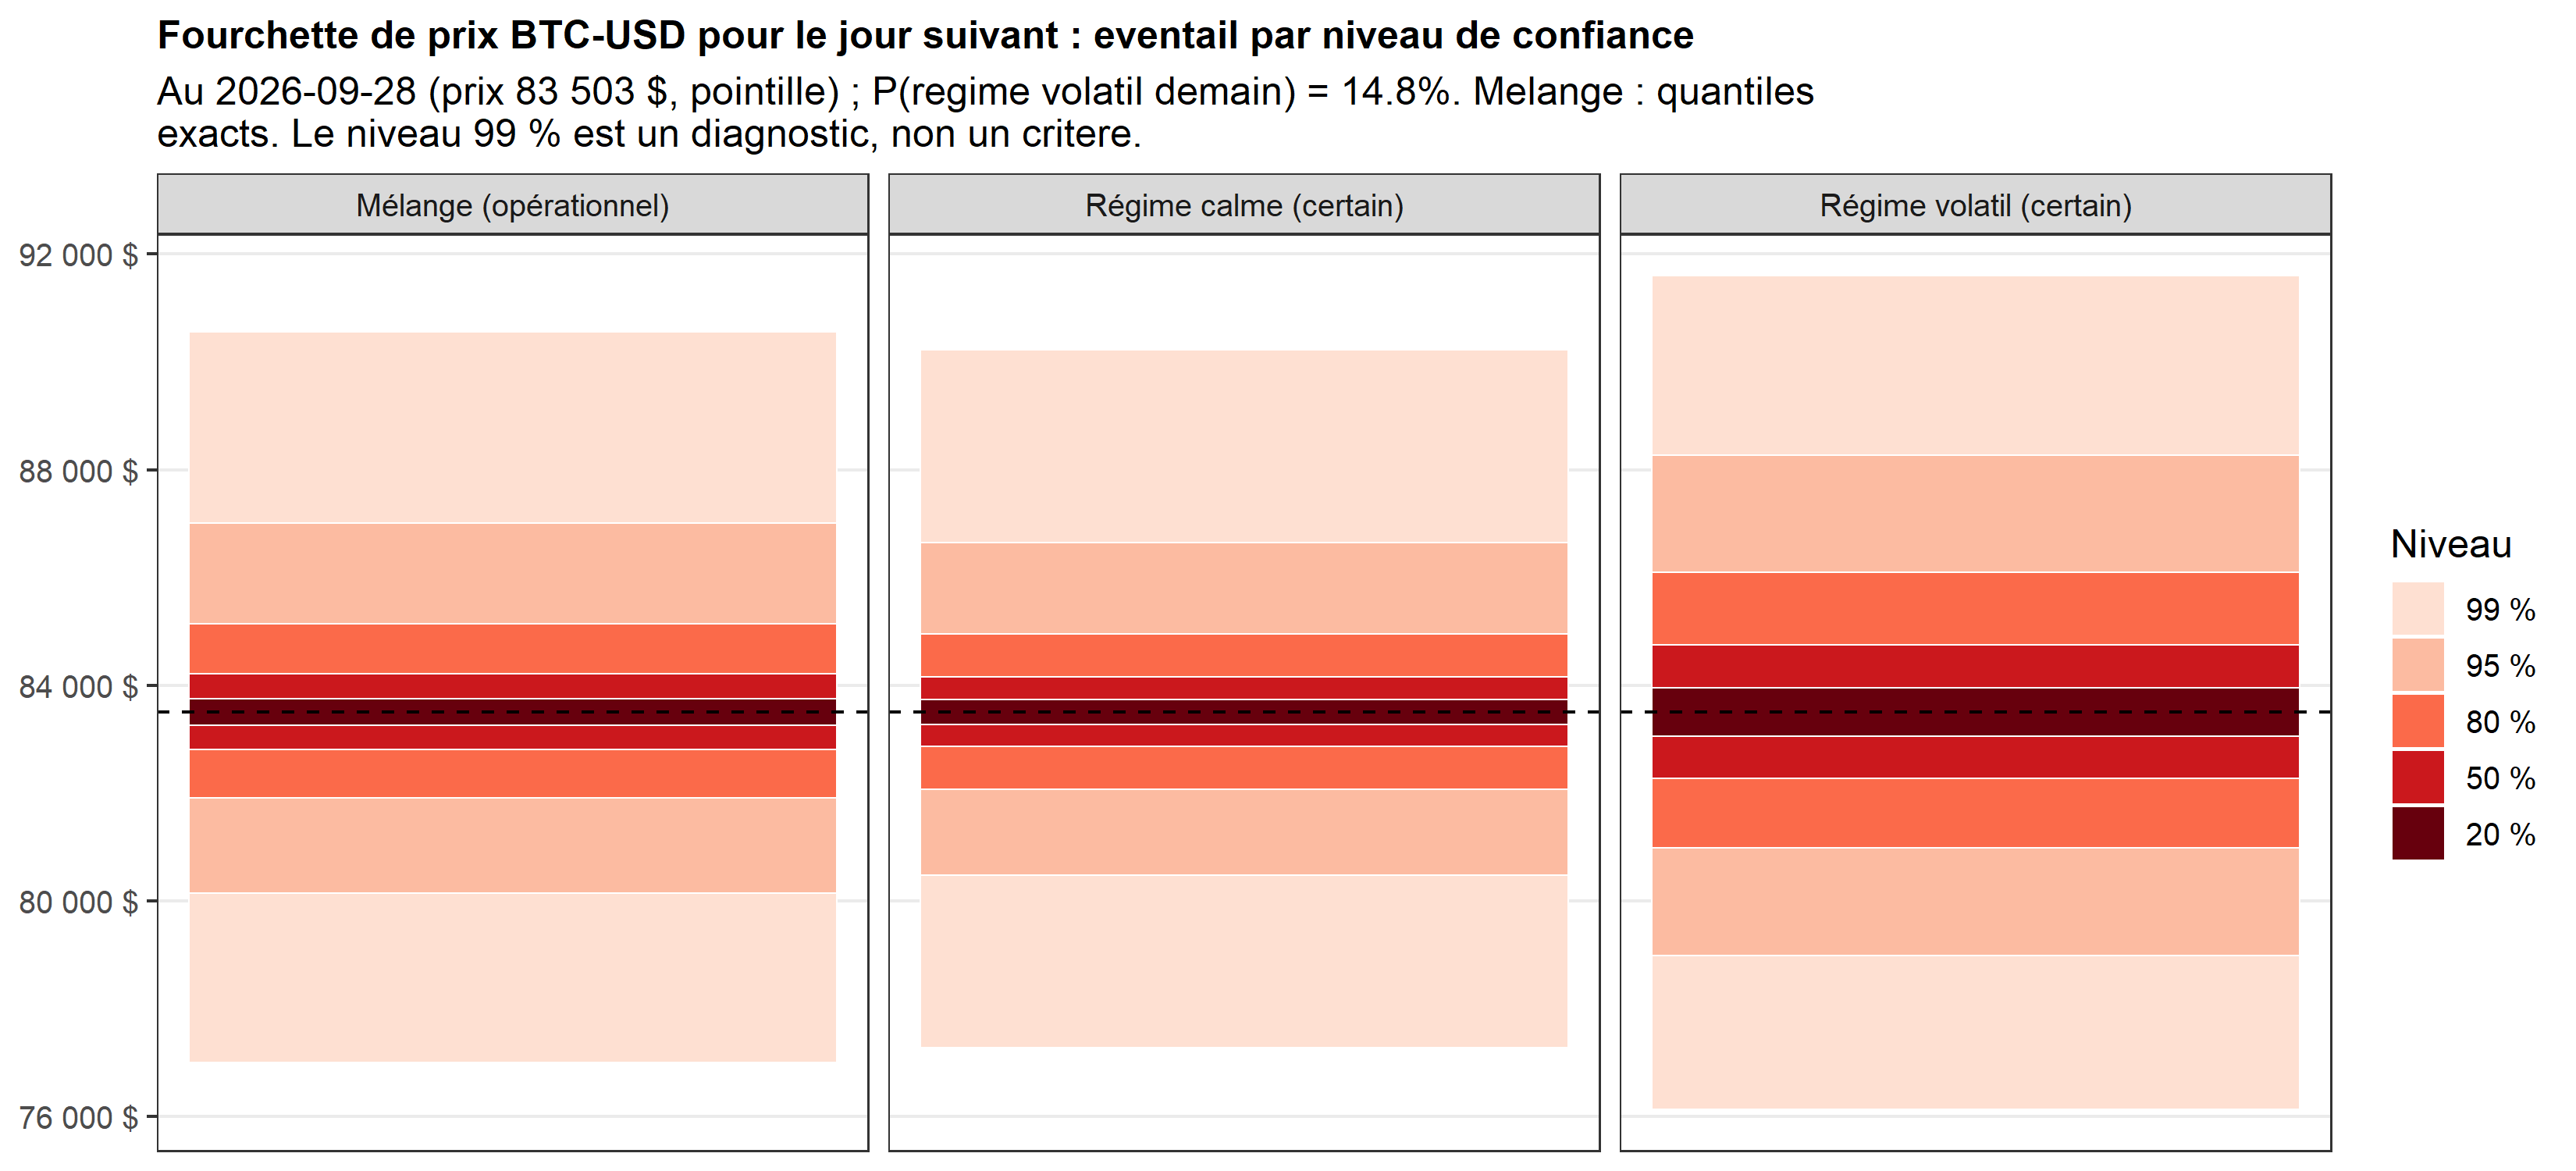
\includegraphics[width=1\linewidth]{10_fan_chart.png}
	\caption{One-day price range for BTC-USD at several confidence levels: the operational mixture, then each regime taken as certain. The 99\,\% level is a diagnostic, not a criterion. Figure labels are in French.}
	\label{fig:fan}
\end{figure}

\subsection{Validation of the variance recursion}

The three candidate initialisations of the recursion (the unconditional variance, the sample variance, the first squared return) all give a mixture volatility of $2.693894\,\%$/day, \textbf{identical to \texttt{predict()\$vol}} (relative gap zero to six decimals). This is no surprise: the influence of the initialisation decays like $\beta^T$ ($\beta\le 0.924$, $T=4{,}394$), that is, it is nil in practice, even for the regime with $\alpha+\beta\approx0.999$. The recursion of \citet{haasmittnikpaolella2004} is thus validated and the choice of initialisation is immaterial.

\subsection{The range of each regime (each taken as certain)}

\begin{table}[H]
	\centering
	\caption{Range width by regime (in \% of return), one day ahead}
	\label{tab:range-regimes}
	\begin{tabular}{lrrr}
		\toprule
		& Volatile regime & Calm regime & Ratio \\
		\midrule
		$\sigma_{t+1}$ (\%/day) & $2.834$ & $2.669$ & $1.06$ \\
		$\nu$ & $3.95$ & $2.30$ & \\
		Width at 20\,\% & $1.08$ & $0.55$ & $1.96$ \\
		Width at 50\,\% & $2.95$ & $1.54$ & $1.91$ \\
		Width at 80\,\% & $6.12$ & $3.46$ & $1.77$ \\
		Width at 95\,\% & $11.11$ & $7.38$ & $1.51$ \\
		Width at 99\,\% & $18.50$ & $15.49$ & $1.19$ \\
		\bottomrule
	\end{tabular}
\end{table}

At this date the conditional scales of the two regimes are almost equal (ratio $1.06$). The differences in width come from the \textbf{tails} ($\nu = 3.95$ against $2.30$), not from the scale: the ``calm'' regime has a narrower 95\,\% band but heavier extremes (the gap narrows at 99\,\%). On EUR/USD the stress regime had a scale almost twice as large; here the weight of the regimes acts on the \emph{shape} of the distribution more than on its scale. $P(\text{volatile})$ is therefore a weak signal of the width of the band. As a reminder, ``volatile'' and ``calm'' are defined by the realised standard deviation on dominant days (section~\ref{sec:ms-labels}), not by the scale of the forecast of the day.

\subsection{The 95\,\% band against the Normal}

With $\sigma = 2.694\,\%$/day, a Normal 95\,\% band would be $\pm5.28\,\%$. The band of the model is $\pm4.10\,\%$, that is $1.53\,\sigma$: \emph{narrower} than the Normal at the 95\,\% level and \emph{wider} at the 99\,\% level ($\pm 8.13\,\%$ against $\pm 6.94\,\%$). This is the signature of very heavy tails ($\nu$ between 2.3 and 4): a concentrated body and distant extremes. One consequence to watch in the backtest: the coverage at 95\,\% depends on the correctness of this shape, and clustered breaches (Christoffersen) are possible.

\subsection{Mixture quantiles: \texttt{Risk()} against the exact solution}

\begin{table}[H]
	\centering
	\caption{Quantiles of the mixture (in \% of return): \texttt{Risk()} against the exact solution}
	\label{tab:range-mixture}
	\begin{tabular}{rrrr}
		\toprule
		$\alpha$ & \texttt{Risk()} & Exact & Relative gap \\
		\midrule
		0.005 & $-8.141$ & $-8.107$ & $-0.42\,\%$ \\
		0.025 & $-4.112$ & $-4.115$ & $+0.08\,\%$ \\
		0.10 & $-1.983$ & $-1.934$ & $-2.56\,\%$ \\
		0.25 & $-0.919$ & $-0.843$ & $-9.03\,\%$ \\
		0.40 & $-0.310$ & $-0.298$ & $-4.27\,\%$ \\
		0.60 & $+0.298$ & $+0.298$ & $+0.07\,\%$ \\
		0.75 & $+0.830$ & $+0.843$ & $-1.48\,\%$ \\
		0.90 & $+1.894$ & $+1.934$ & $-2.02\,\%$ \\
		0.975 & $+4.099$ & $+4.115$ & $-0.39\,\%$ \\
		0.995 & $+8.129$ & $+8.107$ & $+0.27\,\%$ \\
		\bottomrule
	\end{tabular}
\end{table}

\texttt{Risk()} relies on a numerical grid. At the levels used in the backtest (95 and 99\,\%) the gap is at most $0.5\,\%$ ($\approx 0.016$ return point, about \$13 on the 95\,\% price): \textbf{no effect on coverage}. At central levels it reaches $-9\,\%$ (the 50\,\% band) and makes the band asymmetric ($-0.919$ against $+0.830$, whereas the exact mixture is symmetric at $\pm0.843$). The central bands of the fan chart are therefore slightly distorted by \texttt{Risk()}, while the 95\,\% range is not. The pipeline keeps \texttt{Risk()} for fidelity with EUR/USD; the fan chart uses the exact quantiles for the bands of the mixture.

\begin{econbox}[What this range is, and what it is not]
	The range is a one-day interval for the \emph{close-to-close log return}, centred on the last close because the mean is zero by construction. It says nothing about where the price will be: it says how large an ordinary day is. A 95\,\% range of about $\pm4\,\%$ (roughly \$3,400 either side of \$83,503) tells an analyst that, if the calibration holds, a close outside it should occur on about one day in twenty; whether it does is tested in section~\ref{sec:backtest}. Its width is the information: it moves with the volatility forecast, and its tails are much heavier than a Normal's, so a move that looks extreme under a Normal can fall within the band at 99\,\%.
\end{econbox}

\subsection{Limits}

\begin{itemize}
	\item \textbf{A single date.} The range of 2026-09-29 is not a validation. No comparison with the realised price is made here (one observation proves nothing); the bar of 2026-09-29 is moreover absent from the downloaded file (section~\ref{sec:data-pipeline}).
	\item The model limits of sections~\ref{sec:garch} and~\ref{sec:msgarch} apply: $\nu\le4$ in both regimes, persistence at the boundary, regime probabilities ambiguous for a large share of the days.
	\item The forecast concerns the close-to-close return only; no intraday statistic is used.
\end{itemize}


% ═════════════════════════════════════════════════════════════════
\section{Shock test: January--April 2020}
\label{sec:shock}
% ═════════════════════════════════════════════════════════════════

\subsection{Objective and design}

The question is how a model that has never seen the shock behaves \emph{during} it. The MS-GARCH ($K=2$) is \textbf{re-estimated on the data up to 2019-12-31} (1,931 returns, 2014-09-18 to 2019-12-31), then \textbf{frozen}. A one-day forecast is produced for each of the \textbf{121 days from 2020-01-01 to 2020-04-30} (a seven-day market), with the history extended day by day.

The status of this test was fixed before execution: \textbf{qualitative, outside the success criterion}. A window of about 120 days has no power to validate or invalidate a calibration (section~\ref{sec:backtest} is the test with statistical reach).

The fit uses several starting points (the default one does not find the global optimum, section~\ref{sec:ms-optimum}); the 99\,\% level is also reported; if \texttt{Risk()} fails, the exact mixture is used instead; and the intraday High/Low diagnostic comes from the same source as the closes (\texttt{yfinance}).

\subsection{The model before 2020}

The 19 fits converge to \textbf{the same optimum} (log-likelihood $-4{,}814.95$).

\begin{table}[H]
	\centering
	\caption{MS-GARCH estimated on data up to 2019-12-31}
	\label{tab:shock-pre2020}
	\begin{tabular}{lrr}
		\toprule
		& Volatile regime & Calm regime \\
		\midrule
		Persistence $\alpha+\beta$ & $0.9646$ & $0.9996$ (\textbf{flag $>0.999$}) \\
		$\nu$ (s.e.) & $5.09$ ($1.01$) & $2.37$ ($0.080$) (\textbf{flag $\nu\le4$}) \\
		$P(\text{stay in regime})$ & $0.9748$ & $0.9759$ \\
		\bottomrule
	\end{tabular}
\end{table}

The structure is analogous to that of the full sample (calm: $\nu=2.30$ and persistence $0.999$; volatile: $\nu=3.95$ and $0.988$): it existed before the shock. The tails are \textbf{well identified} (s.e.\ of $\nu$ of $0.08$ for the calm regime): the decade 2014--2019 contains enough extremes to estimate them.

\subsection{Coverage: 121 forecasts, none missing}

\begin{table}[H]
	\centering
	\small
	\caption{Coverage of the frozen model, 2020-01-01 to 2020-04-30 ($n=121$; one-sided binomial test)}
	\label{tab:shock-coverage}
	\setlength{\tabcolsep}{4pt}
	\begin{tabular}{lrrrrr}
		\toprule
		Level & Breaches (exp.) & Coverage & Binomial $p$ & Kupiec $LR$ ($p$) & Christoffersen $p$ \\
		\midrule
		95\,\% & 5 (6.05) & $95.87\,\%$ & $0.729$ & $0.203$ ($0.652$) & $0.510$ \\
		99\,\% (diagnostic) & 1 (1.21) & $99.17\,\%$ & $0.704$ & $0.039$ ($0.843$) & $0.897$ \\
		\bottomrule
	\end{tabular}
\end{table}

With $n=121$ the power is low: a failure to reject is not a validation. The result establishes only that there is \textbf{no collapse of coverage during a major shock}.

\subsection{The breaches at 95\,\%}

\begin{table}[H]
	\centering
	\small
	\caption{The five closing breaches of the 95\,\% range (returns in log-return \%)}
	\label{tab:shock-breaches}
	\begin{tabular}{lrrlrr}
		\toprule
		Date & Return & Lower / upper bound & Side & Excess (pts) & $P(\text{volatile})$ at forecast \\
		\midrule
		2020-01-03 & $+5.02$ & $-4.86$ / $+4.86$ & upper & $0.15$ & $23.9\,\%$ \\
		2020-01-14 & $+8.06$ & $-6.70$ / $+6.65$ & upper & $1.41$ & $76.7\,\%$ \\
		2020-03-08 & $-9.43$ & $-6.32$ / $+6.26$ & lower & $3.11$ & $68.0\,\%$ \\
		2020-03-12 & $\mathbf{-46.47}$ & $-7.07$ / $+7.07$ & lower & $\mathbf{39.40}$ & $50.2\,\%$ \\
		2020-04-29 & $+11.98$ & $-6.55$ / $+6.55$ & upper & $5.44$ & $23.3\,\%$ \\
		\bottomrule
	\end{tabular}
\end{table}

The \emph{frequency} of breaches is correct; their \emph{size} is not. The return of 2020-03-12 is $6.6$ times its lower bound ($-46.5\,\%$ against $-7.1\,\%$), which shows that no 95\,\% band contains such a day. The coverage counts breaches, not their magnitude. The day before, the model was hesitating between the two regimes ($P(\text{volatile})=50.2\,\%$), which agrees with the reading of section~\ref{sec:ms-labels}: the shock is attributed to the calm regime, with its very heavy tails. No breach occurred with $P(\text{volatile})>95\,\%$: and the ``volatile'' label does not mean ``stress'' anyway (section~\ref{sec:ms-labels}).

\begin{figure}[H]
	\centering
	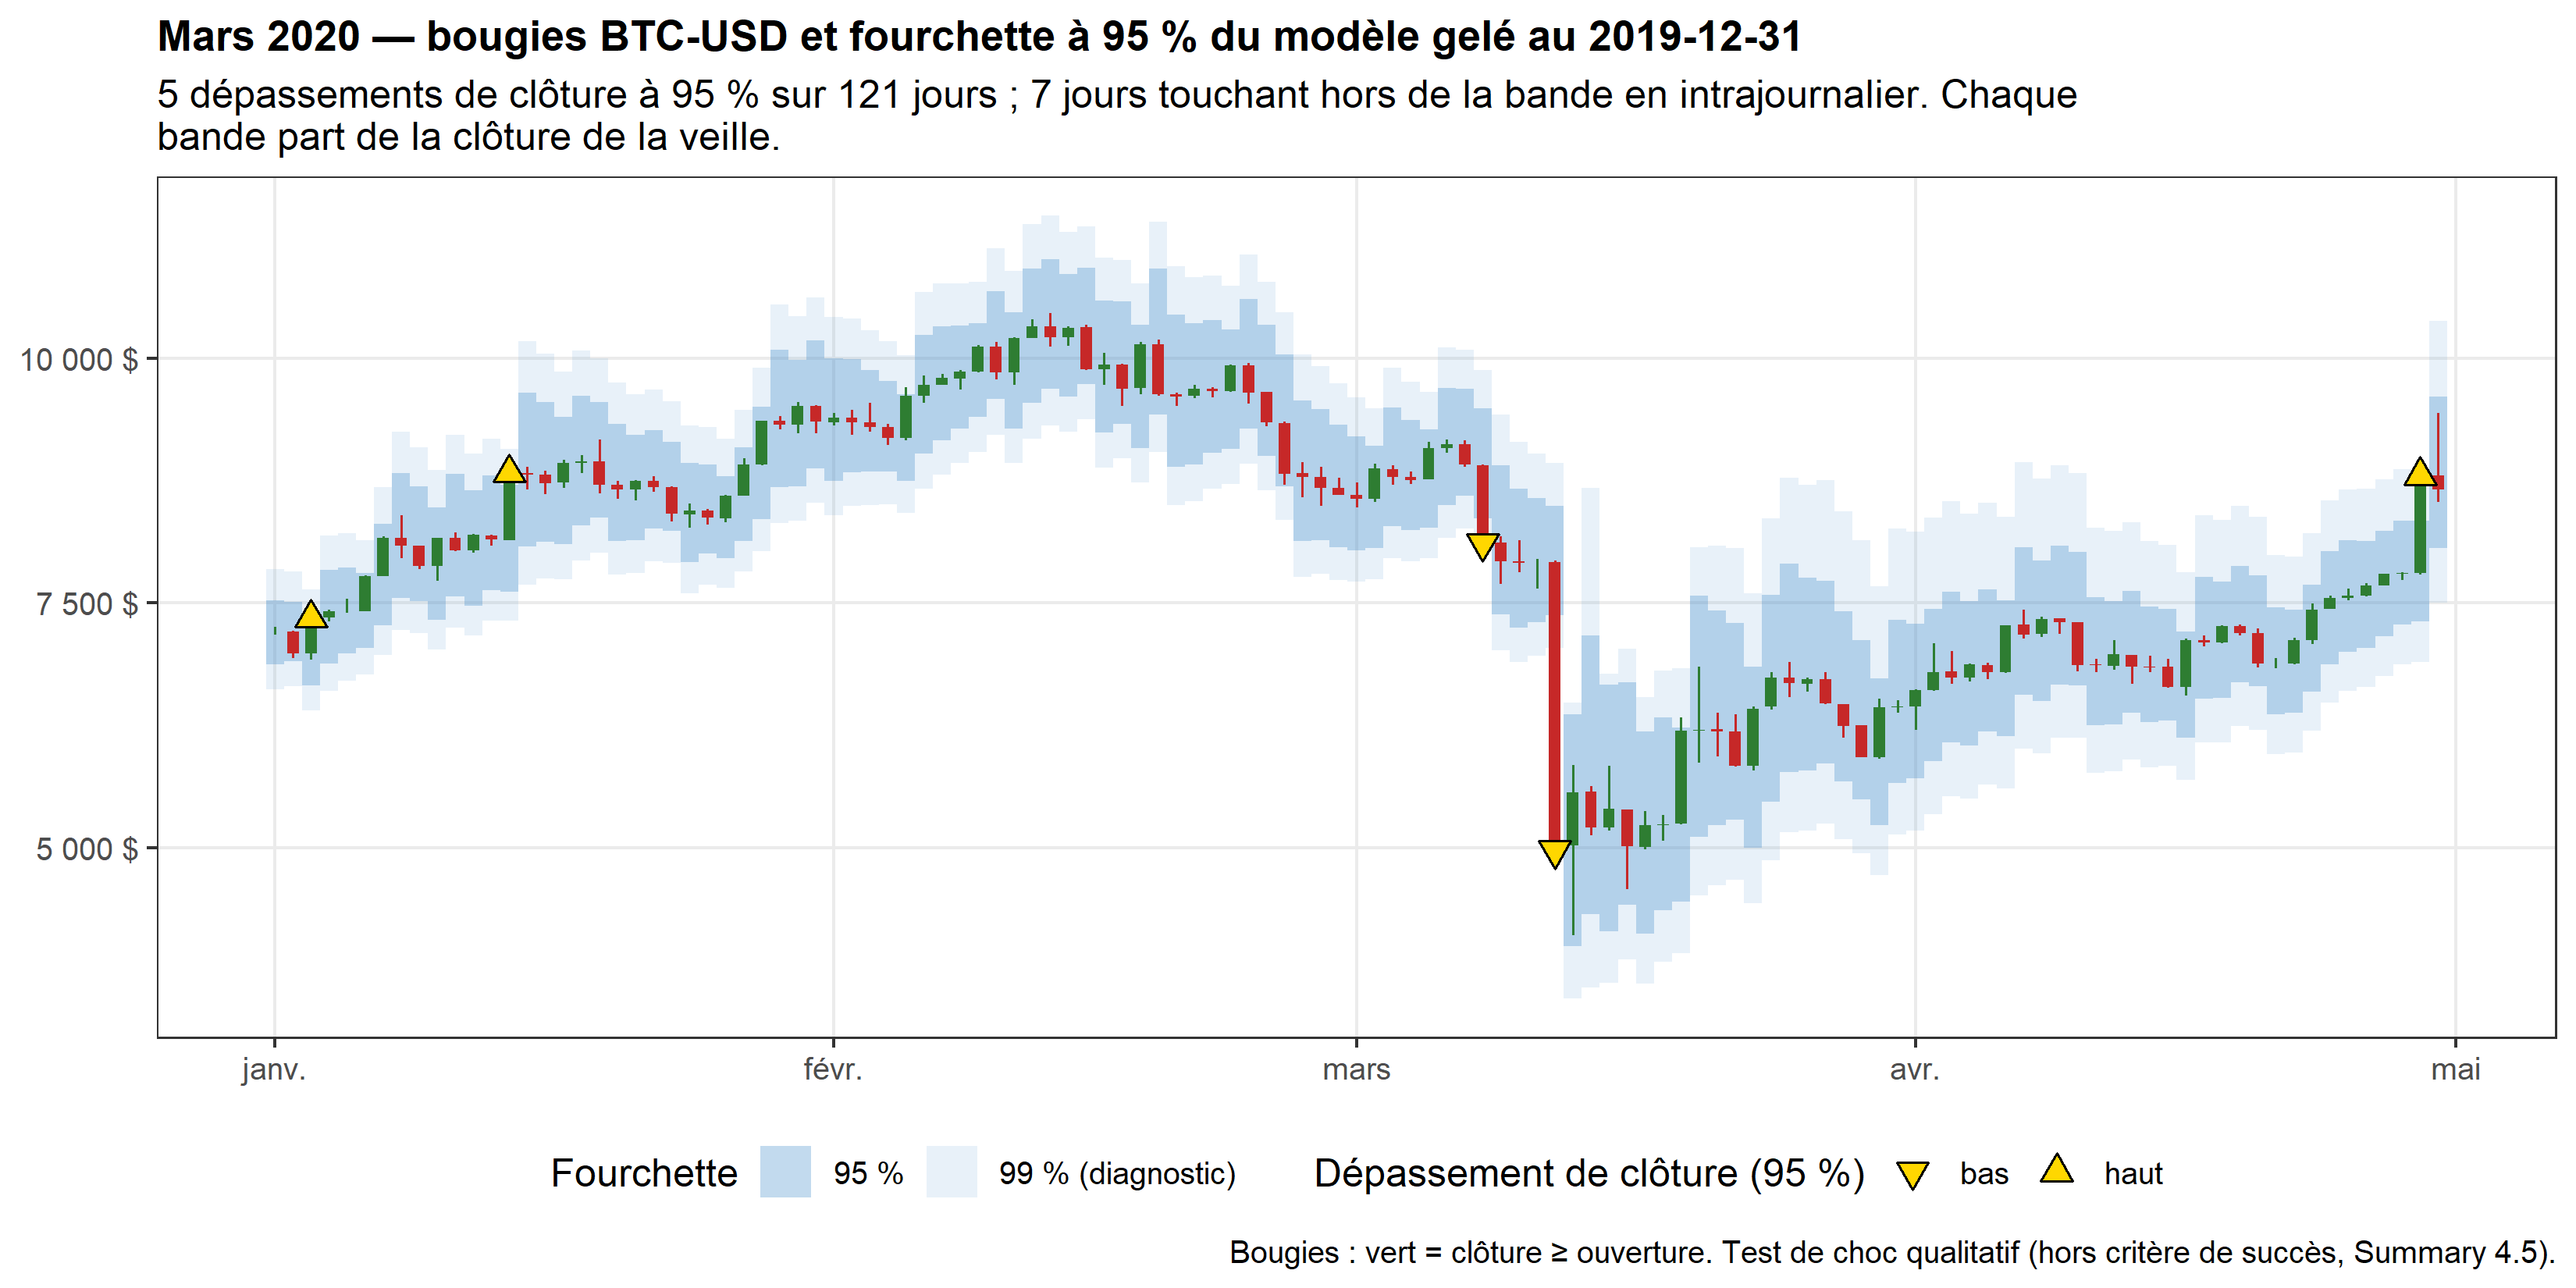
\includegraphics[width=1\linewidth]{11_covid_candlestick.png}
	\caption{BTC-USD candles in March 2020 with the 95\,\% range of the model frozen on 2019-12-31. Triangles mark closing breaches; each band starts from the previous close. Qualitative shock test, outside the success criterion. Figure labels are in French.}
	\label{fig:shock-candles}
\end{figure}

\begin{econbox}[The range reacts after the shock, not before]
	The width of the 95\,\% range was $14.1$ log-return points on the forecast for 2020-03-12, the day of the crash. It rose to $46.7$ points on the next day and peaked at $50.6$ points on 2020-03-14. The model widens; it does not anticipate. For an analyst, a band built from past volatility says how large an ordinary day is \emph{given what has just happened}. It says nothing in advance about the day on which that information changes.
\end{econbox}

\subsection{The forecast of 2020-03-14}

On 2020-03-14, two days after the largest shock, \texttt{Risk()} returned \emph{inconsistent} quantiles ($-37.74$; $-24.03$; $+26.48$; $+26.48$), the upper bounds at 95 and 99\,\% being \emph{identical}: saturation of the numerical grid at its upper bound, after a shock that carried the conditional variance to an extreme level. The exact mixture is used instead (the variance recursion is validated in section~\ref{sec:price-range}): bounds of $\pm25.28\,\%$ at 95\,\%. The realised return, $-6.75\,\%$, lies \emph{inside} the band, so the fallback does not alter the count of breaches.

\subsection{Intraday diagnostic (95\,\%, not decisive)}

Counting the days on which the close, the High or the Low falls outside the band gives \textbf{7 days out of 121} ($5.8\,\%$): the 5 closing breaches plus 2 further days (the High lies above the upper bound on 5 days and the Low below the lower bound on 2).

On a seven-day market, the close at midnight UTC is a snapshot of a market that never closed: the High and the Low of the day bound the same trajectory as the close-to-close return, so the intraday gap is small. The return is measured against the close of the previous day.

\subsection{Limits}

\begin{itemize}
	\item \textbf{One shock, 121 days}: low power. The test is qualitative and outside the success criterion; the test with statistical reach is in section~\ref{sec:backtest}.
	\item \textbf{The coverage counts breaches, not their size.}
	\item \textbf{The grid of \texttt{Risk()} saturates under extreme conditions.} The exact fallback handles this case, but the consistency check detects only non-increasing quantiles: a saturation on a single extreme quantile (for example the 99.5\,\% one) could go unnoticed.
	\item The labels ``volatile'' and ``calm'' do not mean ``crisis'' and ``non-crisis''.
\end{itemize}


% ═════════════════════════════════════════════════════════════════
\section{Full expanding-window backtest (2018--2026)}
\label{sec:backtest}
% ═════════════════════════════════════════════════════════════════

\subsection{Objective and criteria}

This is the pass/fail of the study: are the one-day 95\,\% ranges of the MS-GARCH ($K=2$) \textbf{calibrated} on Bitcoin, out of sample? The criterion was fixed before any estimation and is applied mechanically by the script.

\begin{table}[H]
	\centering
	\caption{Success criterion for the price range (fixed before any estimation)}
	\label{tab:bt-criterion}
	\begin{tabular}{ll}
		\toprule
		Condition & Threshold \\
		\midrule
		Out-of-sample forecasts & $n\ge 2{,}500$ \\
		Unconditional coverage & Kupiec test \citep{kupiec1995}, two-sided, not rejected at 5\,\% \\
		Independence of breaches & Christoffersen test \citep{christoffersen1998}, not rejected at 5\,\% \\
		\bottomrule
	\end{tabular}
\end{table}

Two further quantities are reported \emph{without} pass/fail: the coverage at 99\,\%, and the one-sided binomial test used on EUR/USD (for comparability). There is no ``grey zone'': any coverage rejected by the test is a failure. A known cost is assumed and documented, not corrected: two tests at 5\,\% give about 10\,\% risk of a false rejection for a perfectly calibrated model.

\subsection{Design}

The initial estimation window is 2014-09-18 to 2017-12-31 (1,201 returns). The test runs year by year from 2018 to 2026 (2026 is partial, up to 2026-09-28): \textbf{9 folds and 3,193 forecasts}. On each 1 January the model is re-estimated on \emph{all prior history} (an expanding window, \citealt{west1996}) and its parameters are \textbf{frozen} for the year; each day, the filter and the forecast use the history up to the previous day. No future information enters, which was checked in the code (estimation on dates before 1 January; forecast from the returns up to the day before).

The declared differences with the EUR/USD design are: returns in \% with zero mean; a multi-start fit in each fold, with a warm start from the previous fold, nine or ten fits per fold; a fallback to the exact mixture when \texttt{Risk()} fails; the 99\,\% level computed in parallel; and a save after each fold, with resumption. The run takes about 12 minutes.

\subsection{Main result}

\begin{table}[H]
	\centering
	\small
	\caption{Out-of-sample coverage, 2018-01-01 to 2026-09-28 ($n=3{,}193$)}
	\label{tab:bt-main}
	\setlength{\tabcolsep}{4pt}
	\begin{tabular}{lrrrrr}
		\toprule
		Level & Breaches (exp.) & Coverage & Binom.\ $p$ & Kupiec $LR$ ($p$) & Christ.\ $LR$ ($p$) \\
		\midrule
		\textbf{95\,\%} & 156 (159.7) & $\mathbf{95.11\,\%}$ & $0.628$ & $0.088$ ($\mathbf{0.766}$) & $0.261$ ($\mathbf{0.610}$) \\
		99\,\% (diagnostic) & 27 (31.9) & $99.15\,\%$ & $0.833$ & $0.811$ ($0.368$) & $1.455$ ($0.228$) \\
		\bottomrule
	\end{tabular}
\end{table}

There are 3,193 forecasts, no failure, and one exact fallback (2020-03-14). The 156 breaches at 95\,\% split into 72 below the range and 84 above (symmetry test: $p=0.38$).

\textbf{Verdict on the criterion: PASS.} $n=3{,}193\ge2{,}500$; Kupiec $p=0.766$; Christoffersen $p=0.610$.

\textbf{Precision.} The Wilson 95\,\% interval of the breach rate is $[4.19\,\%\,;\,5.69\,\%]$, i.e.\ a coverage in $[94.3\,\%\,;\,95.8\,\%]$. The Kupiec test rejects only outside about $[94.2\,\%\,;\,95.8\,\%]$: it does not distinguish $95.0\,\%$ from $94.5\,\%$ or $95.7\,\%$.

\begin{figure}[H]
	\centering
	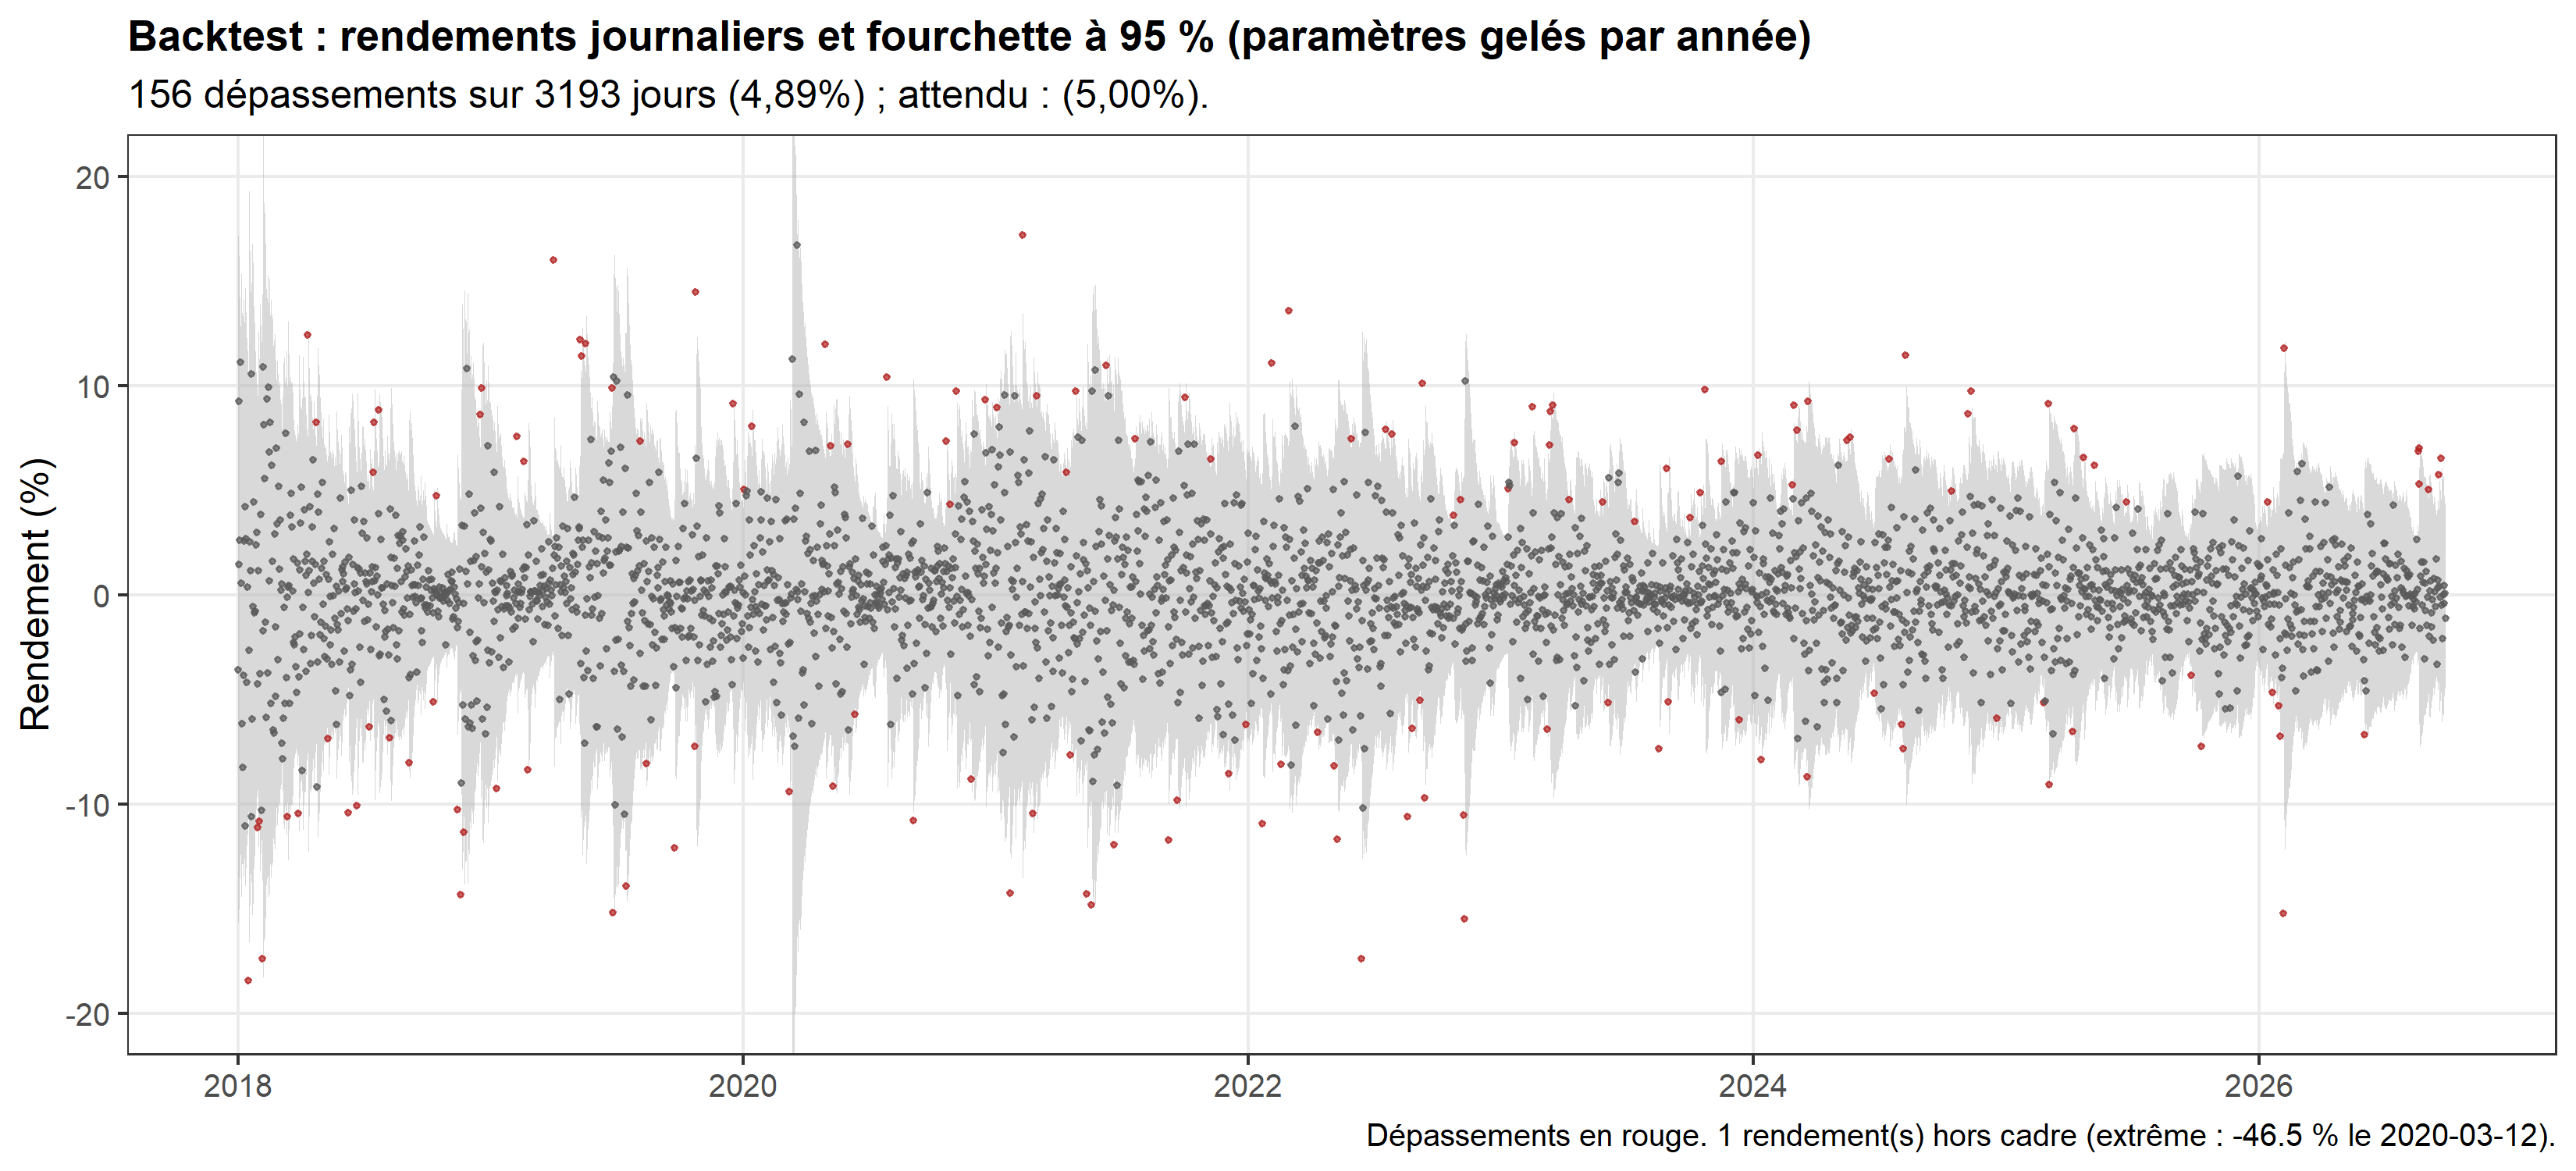
\includegraphics[width=1\linewidth]{12_backtest_returns_vs_band.png}
	\caption{Daily log returns and the 95\,\% range, 2018--2026 (parameters frozen by year). Breaches are in red; one return ($-46.5\,\%$ on 2020-03-12) lies outside the frame. Figure labels are in French.}
	\label{fig:bt-returns}
\end{figure}

\begin{figure}[H]
	\centering
	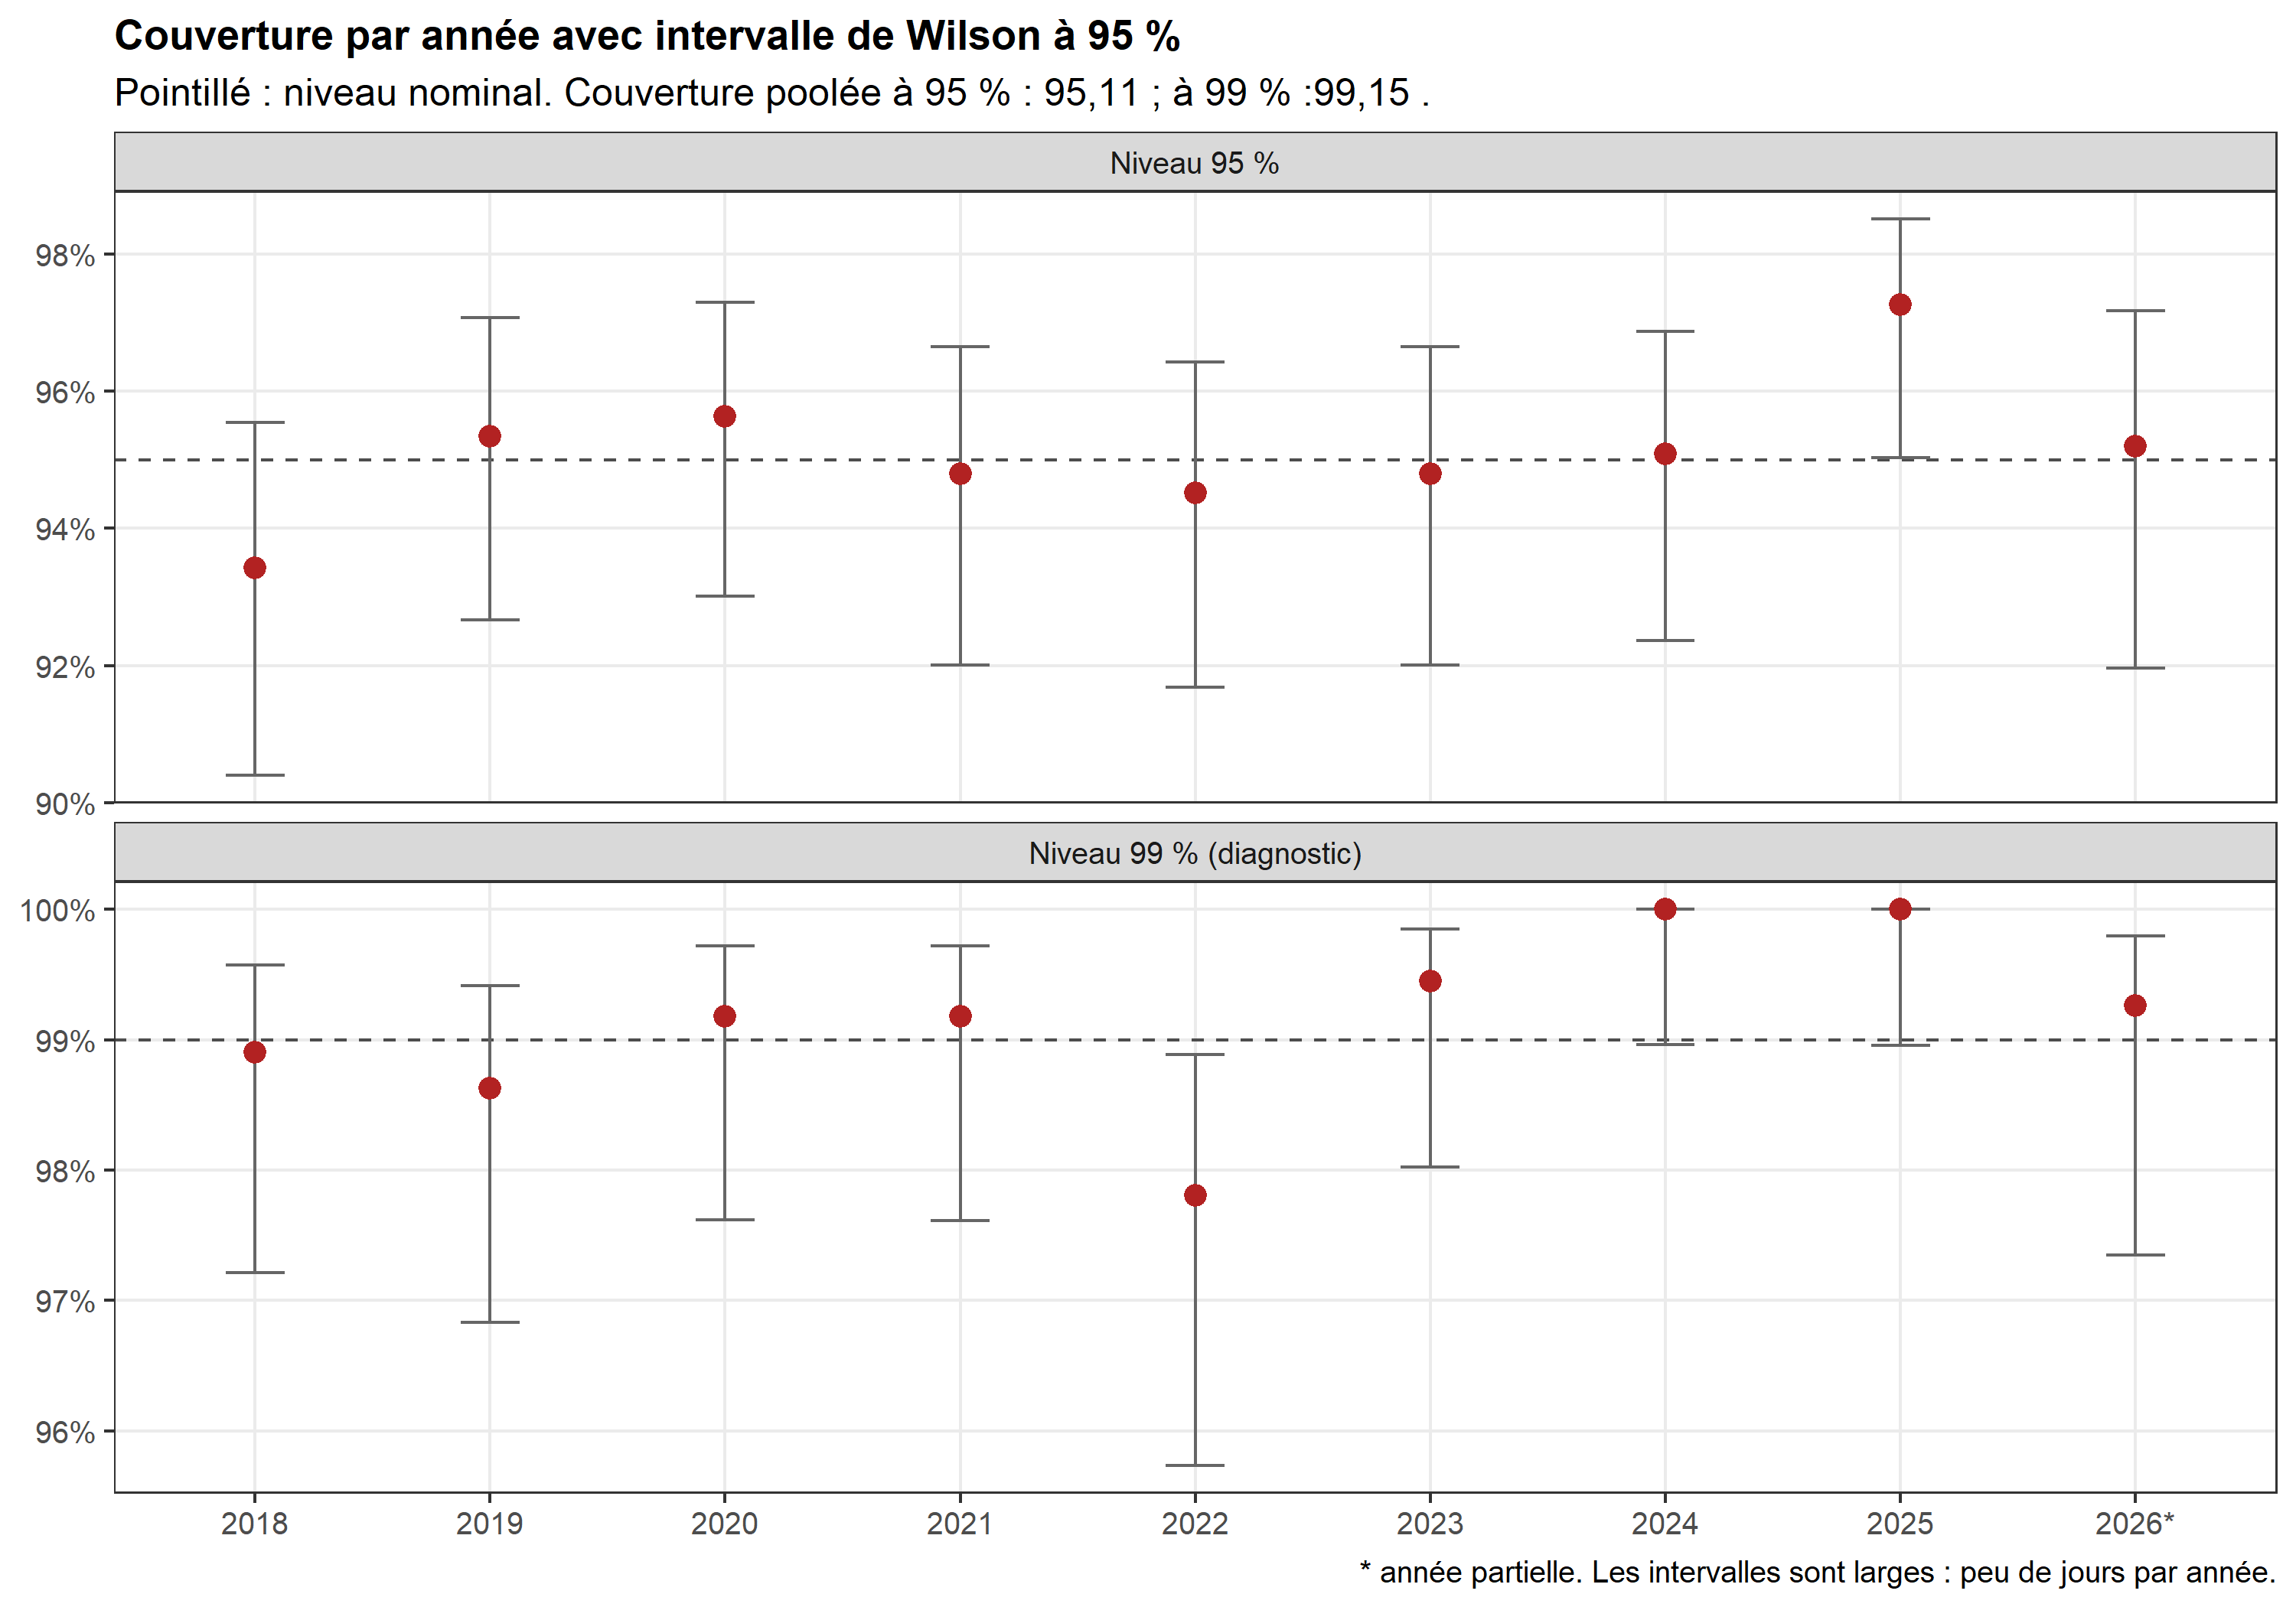
\includegraphics[width=1\linewidth]{13_coverage_by_year.png}
	\caption{Coverage by year with Wilson 95\,\% intervals; the dotted line is the nominal level. The intervals are wide: there are few days per year, and 2026 is partial. Figure labels are in French.}
	\label{fig:bt-coverage-year}
\end{figure}

\begin{figure}[H]
	\centering
	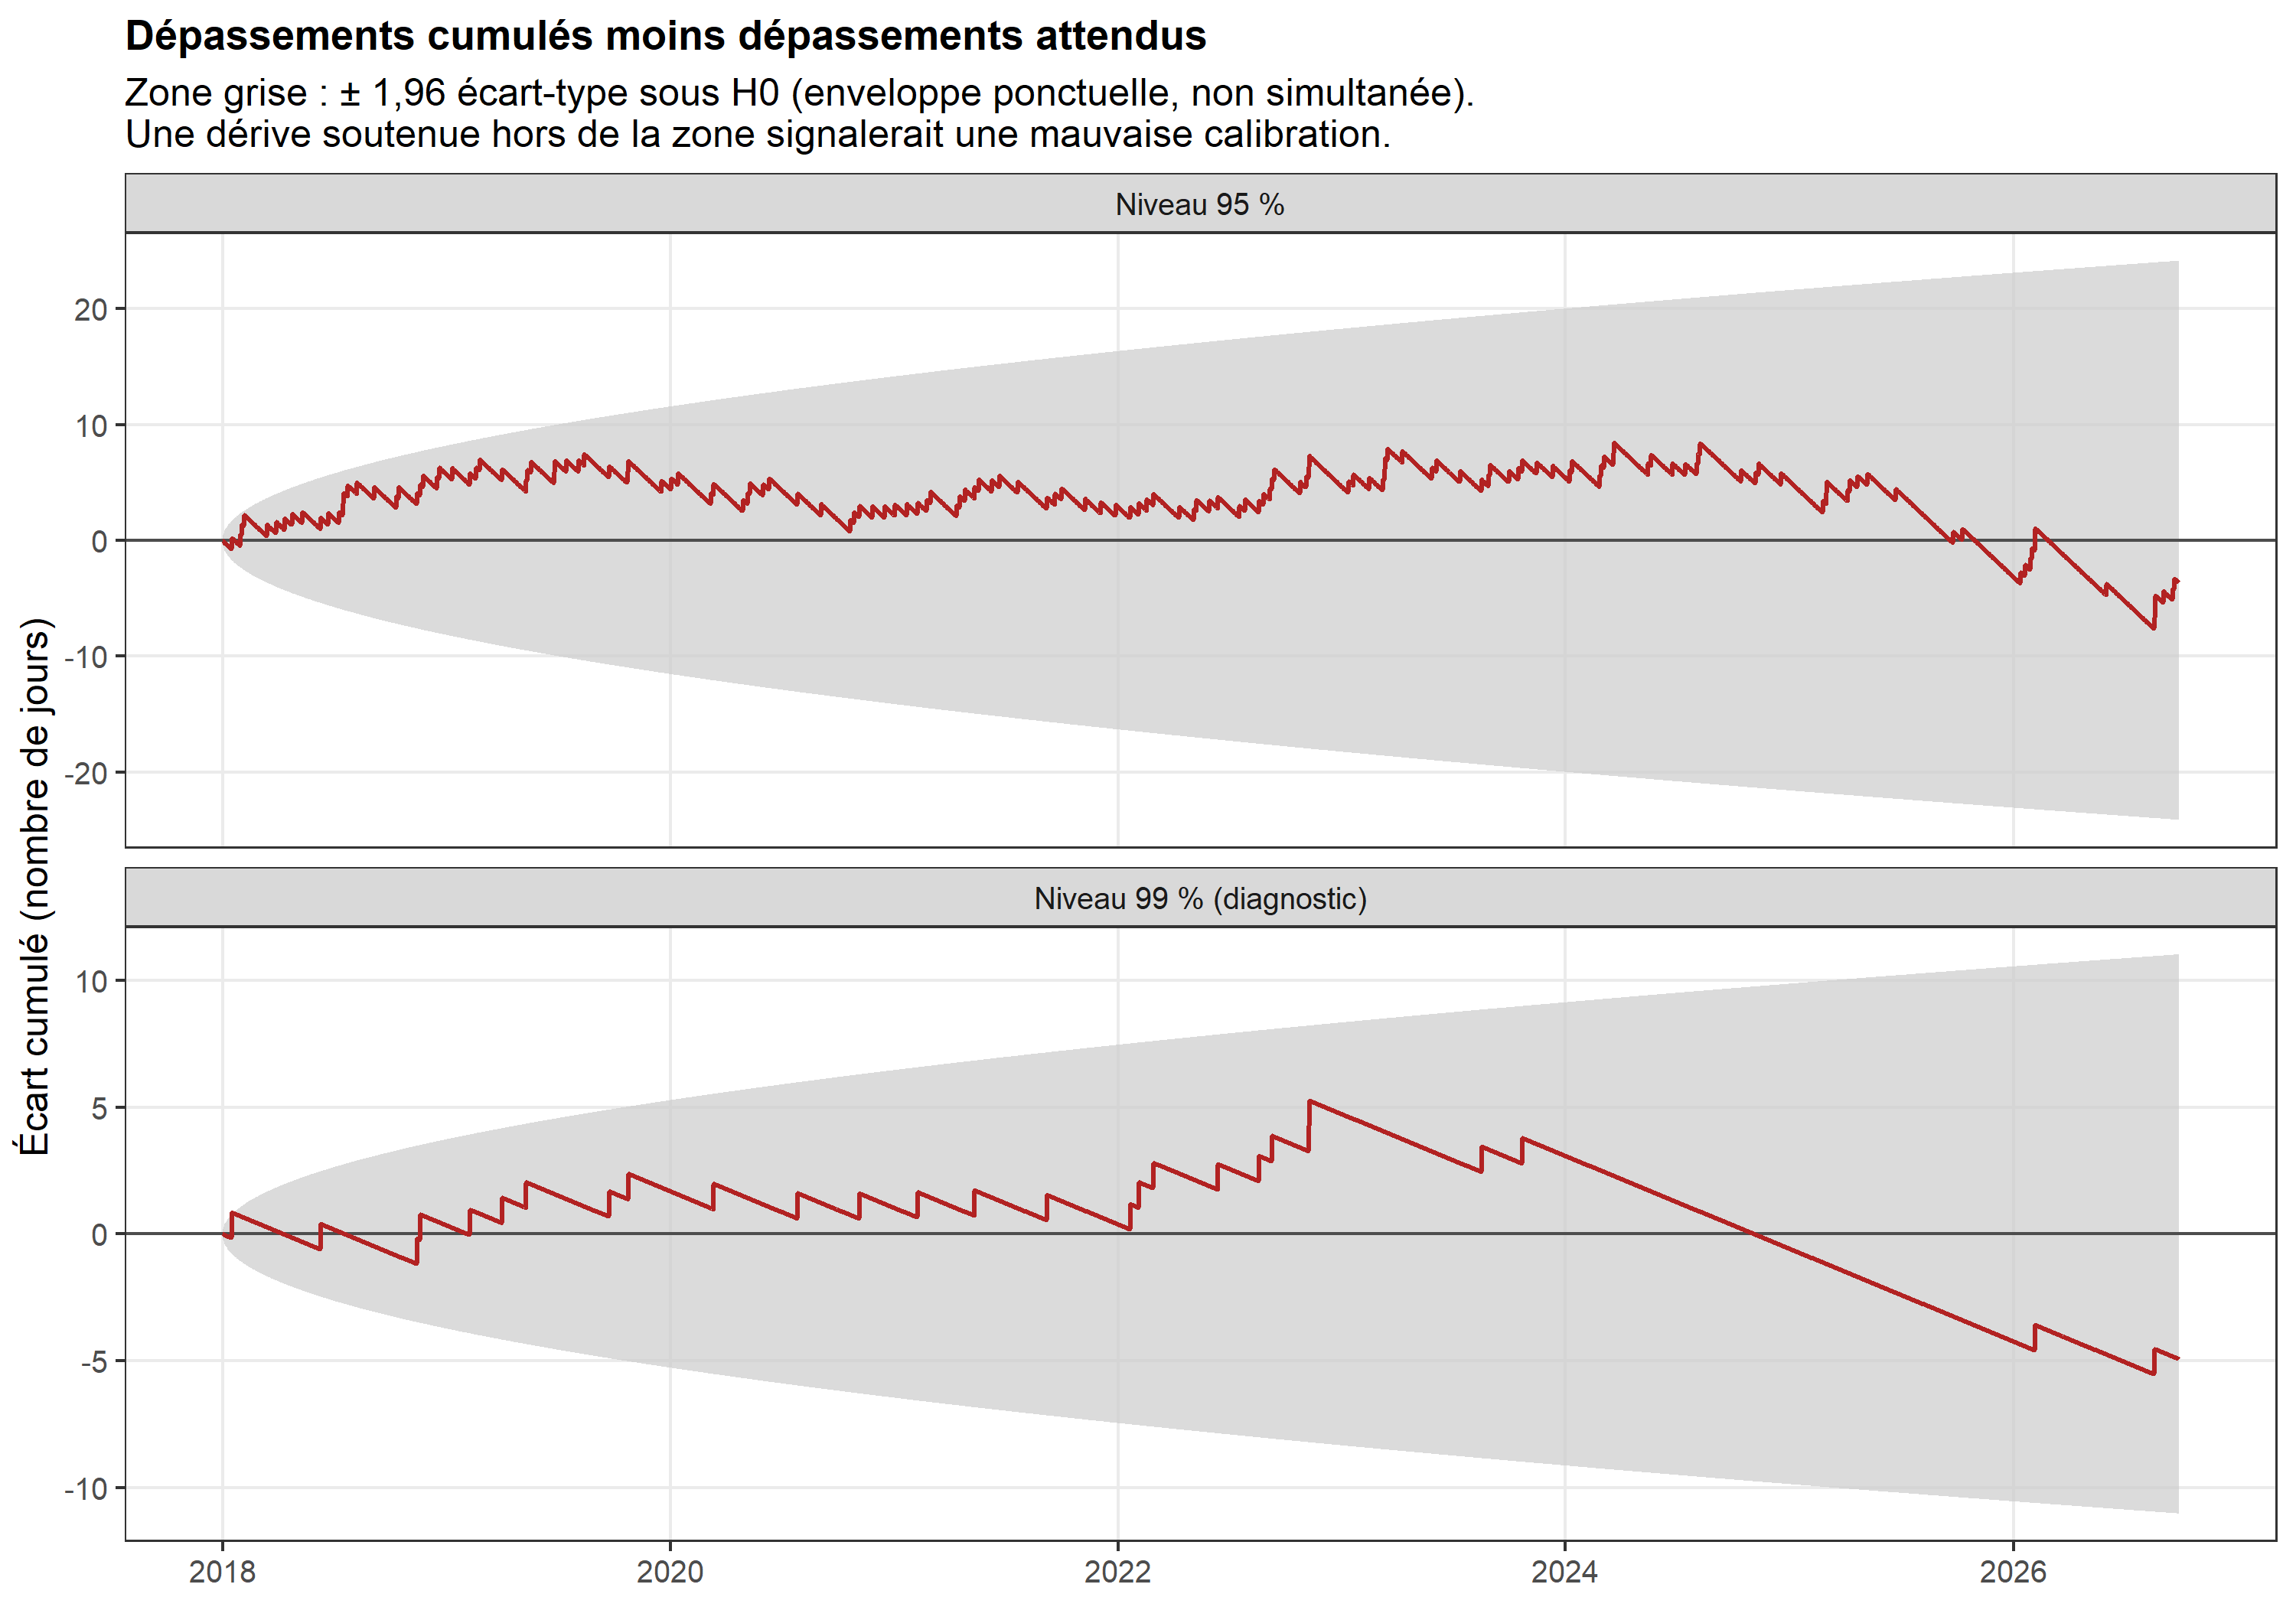
\includegraphics[width=0.95\linewidth]{14_cumulative_breaches_vs_expected.png}
	\caption{Cumulative breaches minus expected breaches. The grey zone is $\pm1.96$ standard deviations under the null (a pointwise, not simultaneous, envelope). A sustained drift outside it would signal a miscalibration. Figure labels are in French.}
	\label{fig:bt-cumulative}
\end{figure}

\subsection{Results by fold}

\begin{table}[H]
	\centering
	\small
	\caption{Results by fold (volatile / calm regime for the last two columns)}
	\label{tab:bt-folds}
	\setlength{\tabcolsep}{3pt}
	\begin{tabular}{lrrrrrcc}
		\toprule
		Year & $n$ & Br.\ 95\,\% & Cov.\ 95\,\% & Br.\ 99\,\% & Cov.\ 99\,\% & Persistence & $\nu$ \\
		\midrule
		2018 & 365 & 24 & $93.42\,\%$ & 4 & $98.90\,\%$ & $0.9663$ / $0.9995$ & $5.32$ / $2.38$ \\
		2019 & 365 & 17 & $95.34\,\%$ & 5 & $98.63\,\%$ & $0.9728$ / $0.9997$ & $5.03$ / $2.38$ \\
		2020 & 366 & 16 & $95.63\,\%$ & 3 & $99.18\,\%$ & $0.9646$ / $0.9996$ & $5.09$ / $2.37$ \\
		2021 & 365 & 19 & $94.79\,\%$ & 3 & $99.18\,\%$ & $0.9701$ / $0.9995$ & $4.40$ / $2.36$ \\
		2022 & 365 & 20 & $94.52\,\%$ & 8 & $97.81\,\%$ & $0.9703$ / $0.9994$ & $4.52$ / $2.35$ \\
		2023 & 365 & 19 & $94.79\,\%$ & 2 & $99.45\,\%$ & $0.9700$ / $0.9995$ & $4.18$ / $2.38$ \\
		2024 & 366 & 18 & $95.08\,\%$ & 0 & $100.00\,\%$ & $0.9754$ / $0.9993$ & $4.10$ / $2.35$ \\
		2025 & 365 & 10 & $97.26\,\%$ & 0 & $100.00\,\%$ & $0.9798$ / $0.9994$ & $3.95$ / $2.34$ \\
		2026$^{*}$ & 271 & 13 & $95.20\,\%$ & 2 & $99.26\,\%$ & $0.9837$ / $0.9991$ & $4.07$ / $2.32$ \\
		\bottomrule
	\end{tabular}

	\smallskip
	{\footnotesize $^{*}$ Partial year (to 2026-09-28).}
\end{table}

Flag: the persistence of the calm regime exceeds $0.999$ in \textbf{all nine folds} ($0.9991$ to $0.9997$); no flag on the standard error of $\nu$. The best fit comes sometimes from the warm start (2021, 2024, 2025), sometimes from a ``persistent regime'' start (2018, 2019, 2020, 2023, 2026) and once from the default start (2022): \textbf{no single starting point suffices}.

\textbf{Reproducibility check.} The 2020 fold uses the same training cutoff (2019-12-31, 1,931 returns) as the shock test of section~\ref{sec:shock}, although the two were run in different scripts. The fits coincide: log-likelihood $-4{,}814.95$, persistence $0.9646$ / $0.9996$, $\nu = 5.09$ / $2.37$. This is not guaranteed by construction; it supports the reproducibility of the pipeline.


\subsection{What the sub-periods show (exploratory, not corrected for multiple comparisons)}

\begin{itemize}
	\item \textbf{2018: moderate under-coverage} (24 breaches for 18.2 expected; Kupiec $p=0.19$, not significant). This fold is estimated on only 1,201 returns.
	\item \textbf{2025: over-coverage at 95\,\%} (10 breaches for 18.2; Kupiec $p=0.031$ uncorrected, hence not significant after a correction over nine folds).
	\item \textbf{2022: 8 breaches at 99\,\% for 3.6 expected} (one-sided $p=0.032$, uncorrected).
	\item \textbf{2024--2025: no breach at 99\,\% in 731 days} for 7.3 expected. The probability under the model is $0.0006$ (a grouping chosen after the fact; taking the possible groupings into account, of the order of $0.006$). The 99\,\% bands look too wide in this period of low realised volatility (yearly standard deviation of 2.2 to 2.8\,\%).
\end{itemize}

\textbf{Are these gaps more than noise?} A test that all nine annual breach rates equal the nominal rate gives $\chi^2(9)=6.5$, $p=0.69$ at 95\,\% (the standard deviation of the annual coverages, $1.0$ point, does not exceed the binomial noise expected for 365 days, $1.14$ points), and $\chi^2(9)=14.3$, $p=0.11$ at 99\,\% (a rough approximation: expected counts of 3 to 4 per fold). The gaps by year are \textbf{not established as anything other than sampling noise}. The only pattern worth a follow-up is the absence of 99\,\% breaches in 2024--2025, observed after the fact. None of these observations was planned in the design; they belong to further work.

\subsection{Evolution of the parameters across folds}

\begin{figure}[H]
	\centering
	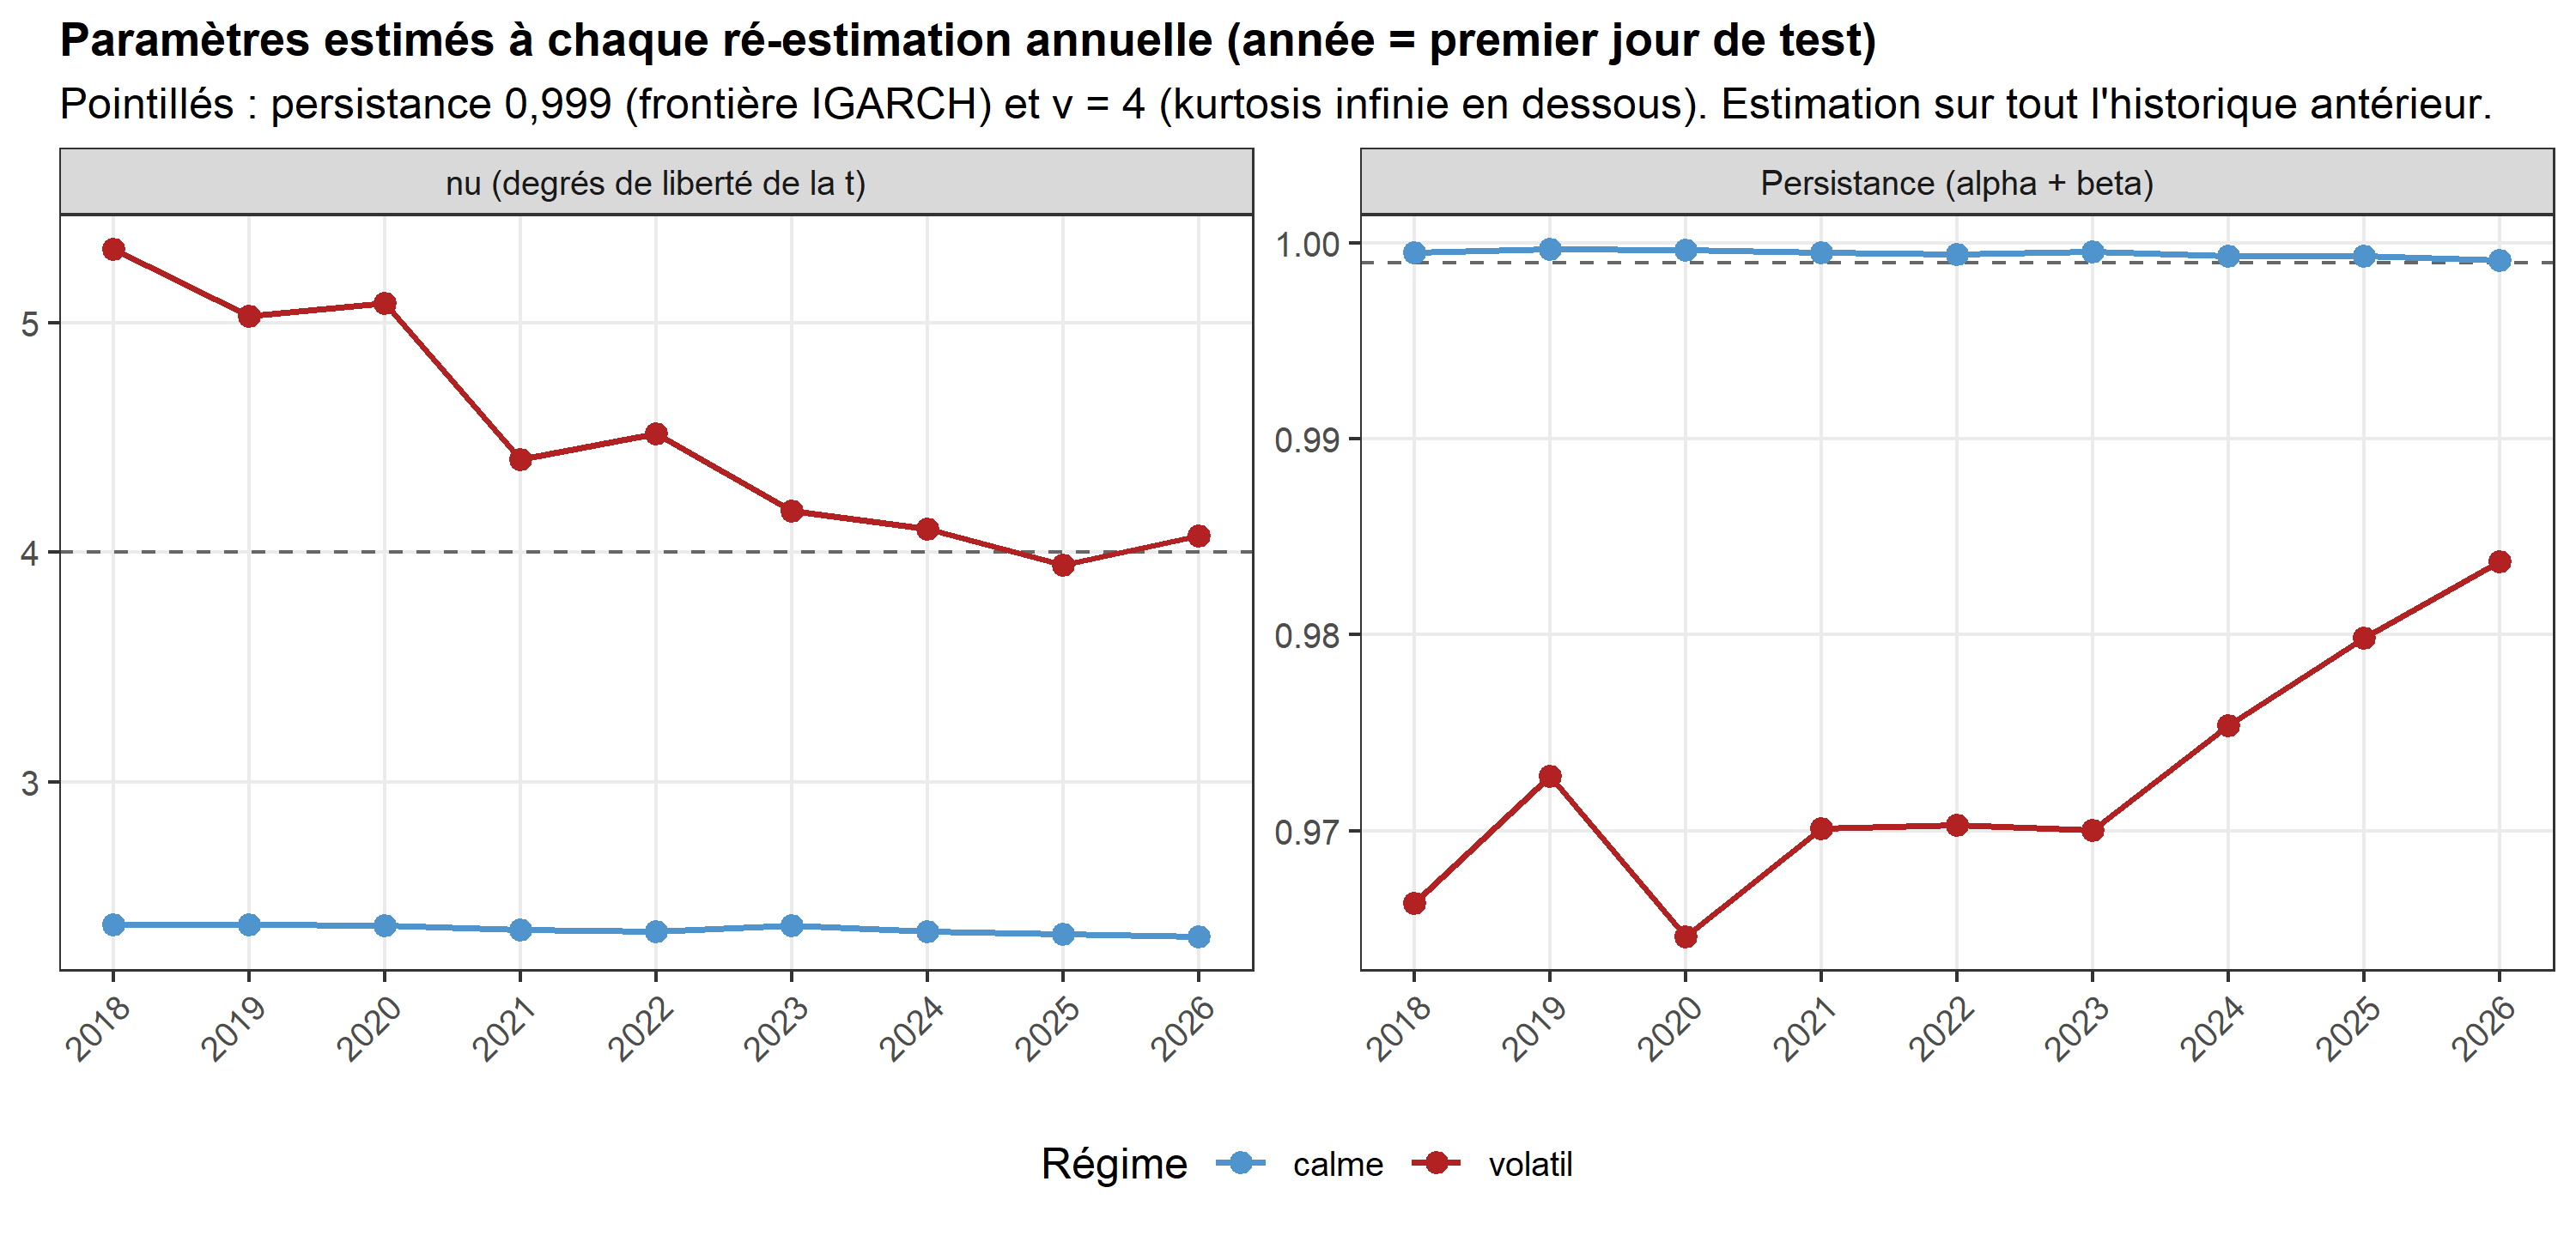
\includegraphics[width=1\linewidth]{16_params_by_fold.png}
	\caption{Parameters estimated at each annual re-estimation (the year is the first day of the test): $\nu$ and persistence by regime. Dotted lines: persistence $0.999$ (IGARCH boundary) and $\nu=4$ (infinite kurtosis below). Estimation on all prior history. Figure labels are in French.}
	\label{fig:bt-params}
\end{figure}

The calm regime is stable: $\nu$ between $2.32$ and $2.38$, persistence between $0.9991$ and $0.9997$ (the boundary) at every fold. The volatile regime moves: $\nu$ falls from $5.3$ (2018) to $4.0$--$4.1$ (2025--2026) and the persistence rises from $0.966$ to $0.984$. With each re-estimation the tails get heavier and the memory longer.

The regimes remain persistent in every fold (Figure~\ref{fig:bt-transition}): the expected duration of the calm regime is 34 to 42 days, and that of the volatile regime 36 to 65 days, lengthening from 2022 (about 36 to 45 days in 2018--2021 and 54 to 65 days from 2022 on). The probability of the volatile regime that oscillates quickly in Figure~\ref{fig:bt-regime-prob} reflects a filter that reacts to returns, not short regimes.

\begin{figure}[H]
	\centering
	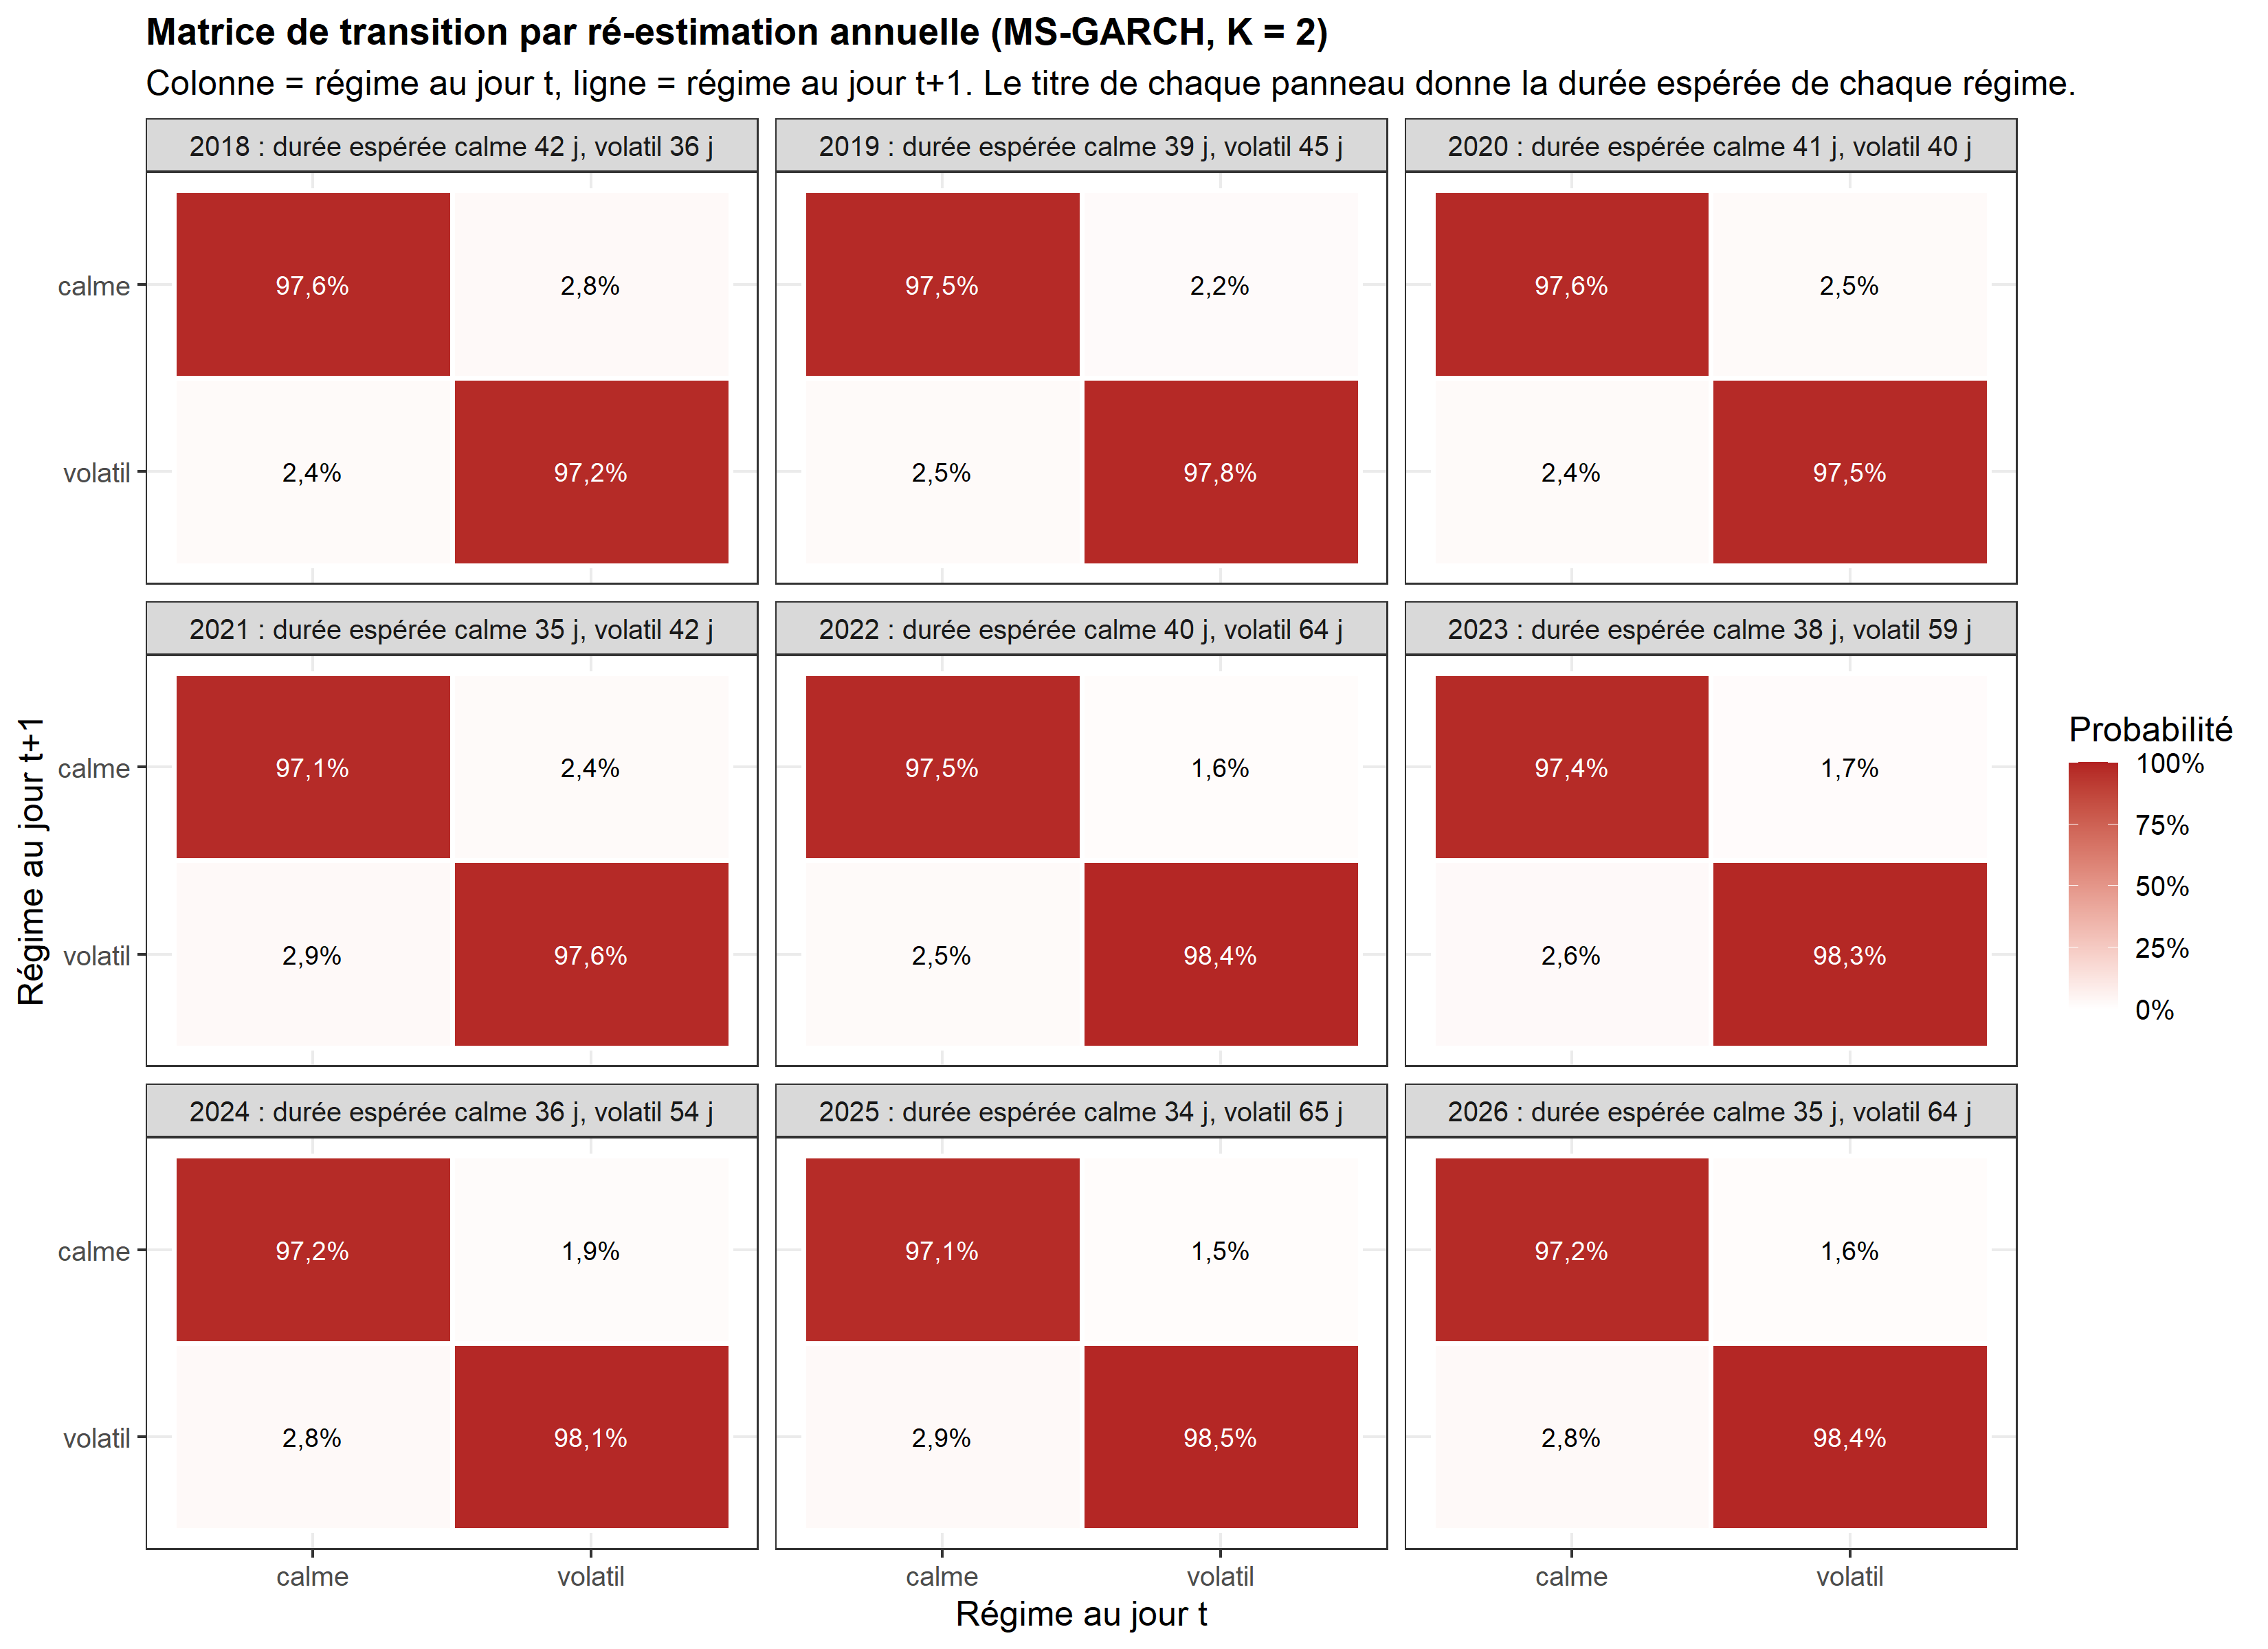
\includegraphics[width=1\linewidth]{17_transition_by_fold.png}
	\caption{Transition matrix at each annual re-estimation. Column $=$ regime on day $t$, row $=$ regime on day $t+1$. The title of each panel gives the expected duration of each regime. Figure labels are in French.}
	\label{fig:bt-transition}
\end{figure}

\textbf{The labels are relative to each re-estimation.} Figure~\ref{fig:bt-sigma} gives the realised standard deviation of each regime, weighted by the regime probability predicted the day before.

\begin{table}[H]
	\centering
	\caption{Realised standard deviation by regime and by test year (\%/day)}
	\label{tab:bt-sigma}
	\begin{tabular}{lrrrr}
		\toprule
		Year & Volatile & Calm & All days & Ratio volatile/calm \\
		\midrule
		2018 & $4.54$ & $3.88$ & $4.29$ & $1.17$ \\
		2019 & $4.11$ & $2.92$ & $3.53$ & $1.41$ \\
		2020 & $3.98$ & $4.02$ & $4.01$ & $0.99$ \\
		2021 & $4.17$ & $4.32$ & $4.20$ & $0.96$ \\
		2022 & $3.62$ & $2.91$ & $3.36$ & $1.24$ \\
		2023 & $2.41$ & $2.12$ & $2.27$ & $1.13$ \\
		2024 & $2.87$ & $2.53$ & $2.78$ & $1.13$ \\
		2025 & $2.33$ & $1.91$ & $2.19$ & $1.22$ \\
		2026$^{*}$ & $2.49$ & $2.31$ & $2.43$ & $1.08$ \\
		\bottomrule
	\end{tabular}
\end{table}

\begin{figure}[H]
	\centering
	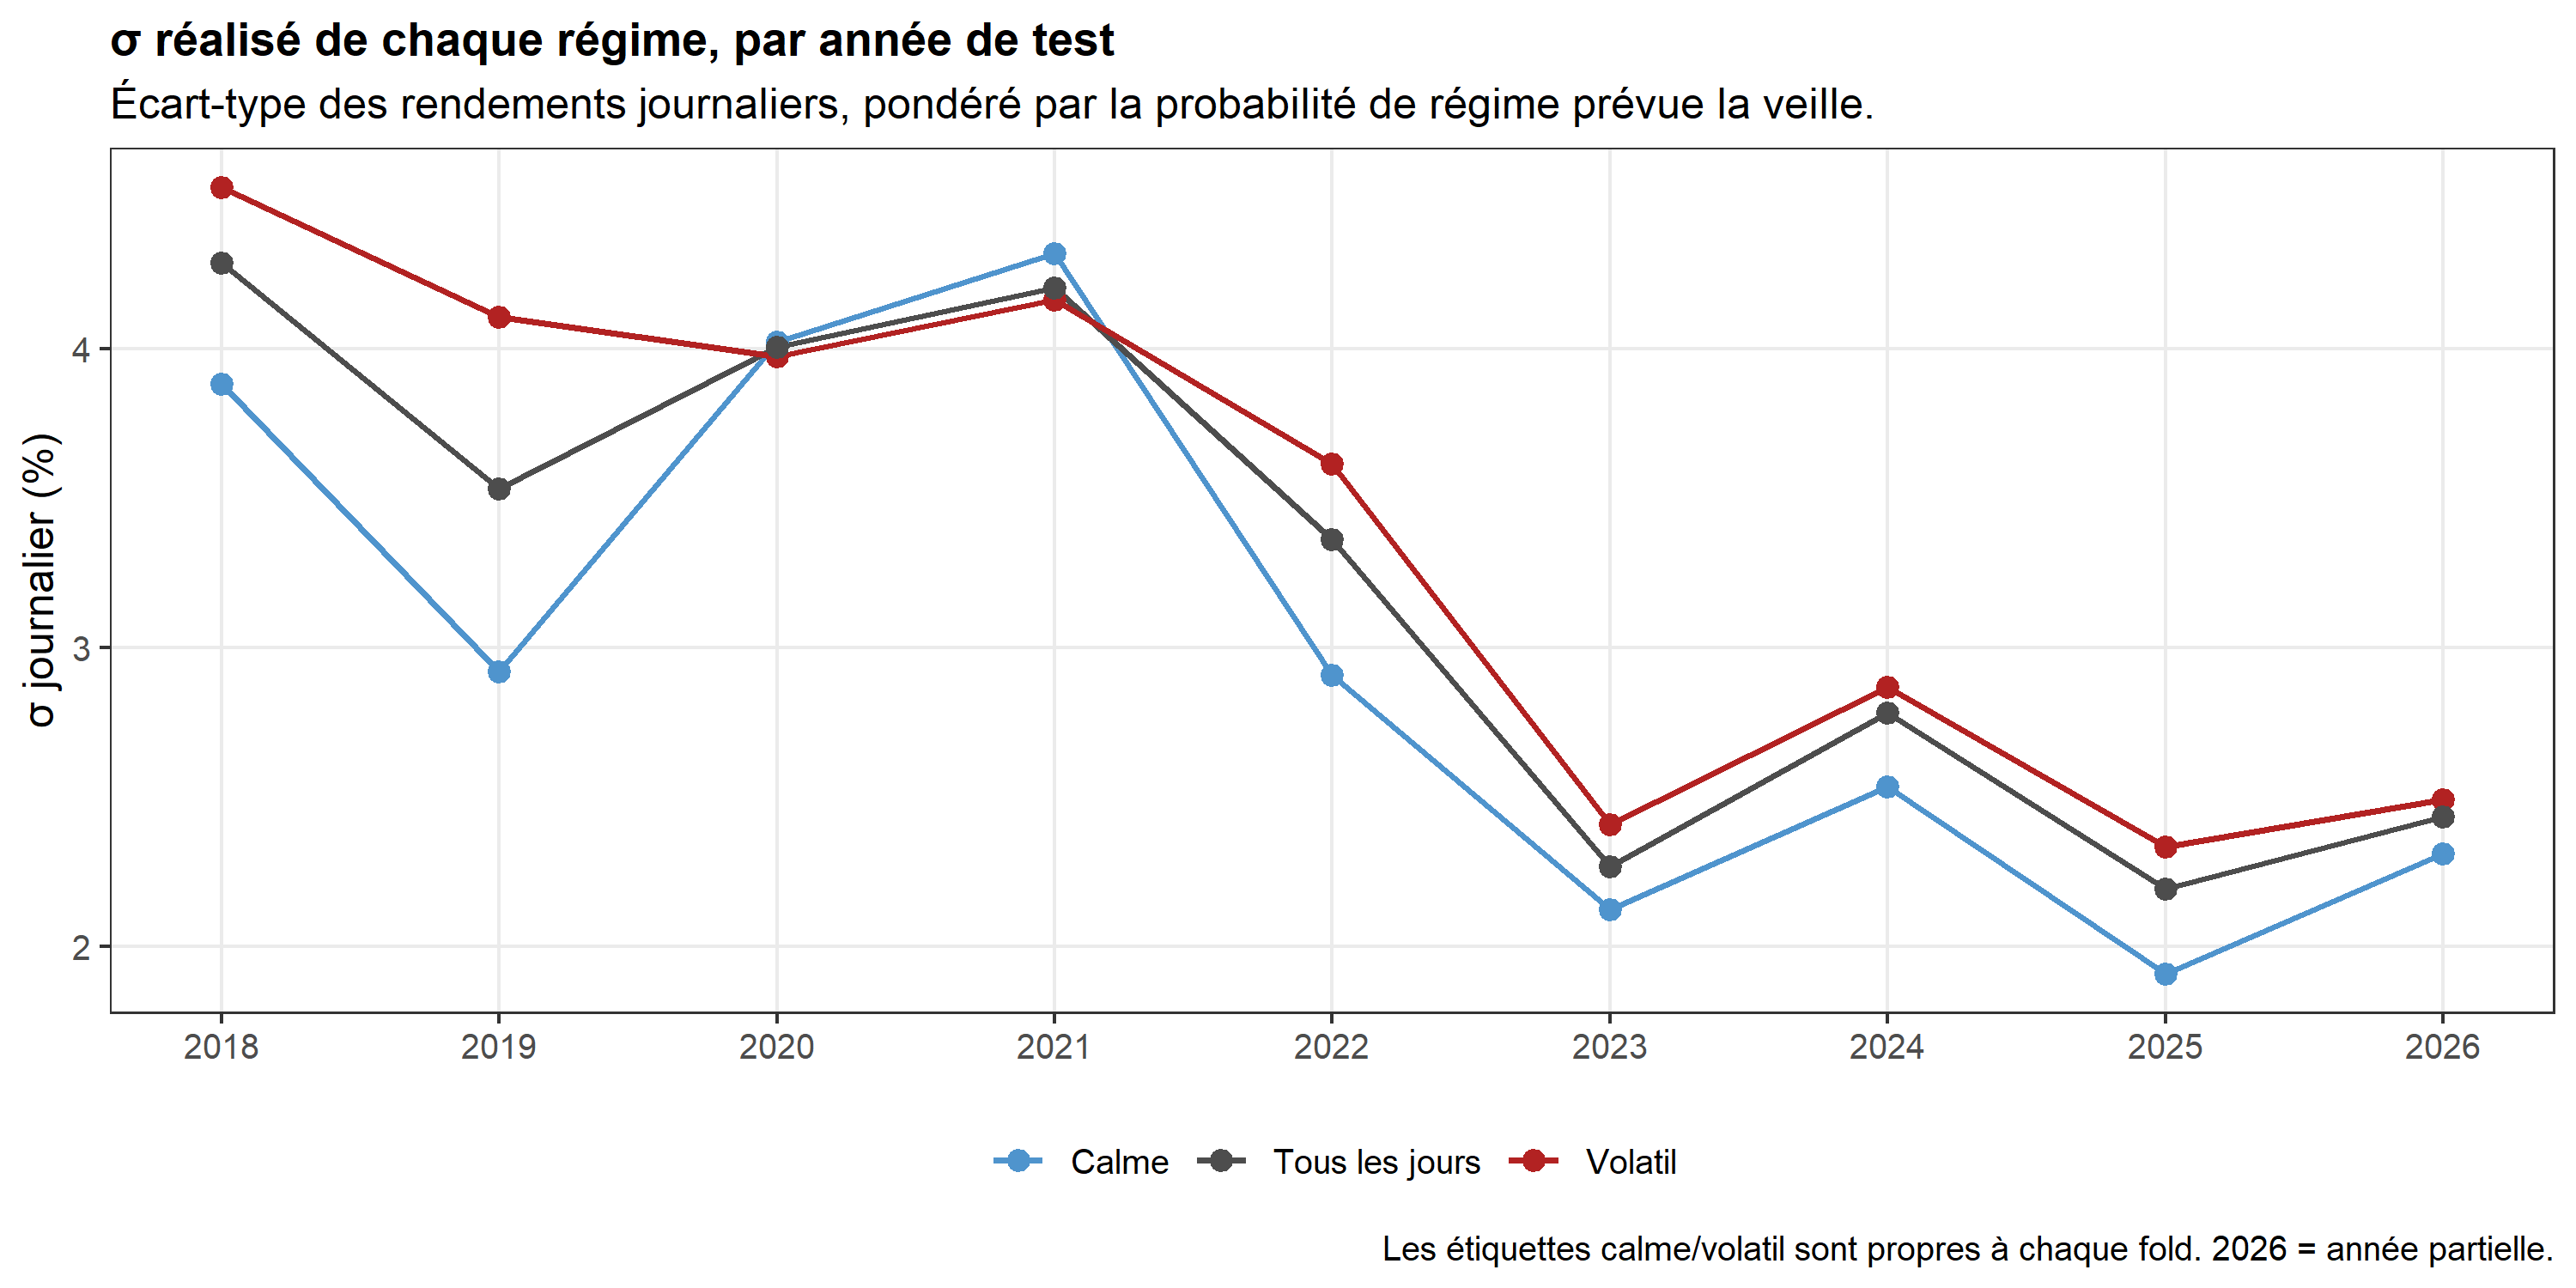
\includegraphics[width=1\linewidth]{18_sigma_by_regime_by_fold.png}
	\caption{Realised standard deviation of each regime by test year, weighted by the regime probability predicted the day before. Regime labels are specific to each fold; 2026 is a partial year. Figure labels are in French.}
	\label{fig:bt-sigma}
\end{figure}

The ``volatile'' regime of 2025 ($2.33\,\%$ per day, about $45\,\%$ annualised) is less volatile than the ``calm'' regime of 2018 ($3.88\,\%$, about $74\,\%$ annualised). In 2020 and 2021 the two regimes do not separate by realised standard deviation ($3.98$ against $4.02$, and $4.17$ against $4.32$, the ``volatile'' one being slightly \emph{below} the ``calm'' one); no test and no standard error were computed for these differences, so they are read as ``no separation'', not as a demonstrated inversion. The labels are therefore properties of each re-estimation: ``volatile'' does not mean a high level of risk in itself, and the regimes of different years are not compared.

\subsection{The day of the fallback}

On 2020-03-14, \texttt{Risk()} returns inconsistent quantiles (saturation of the grid after the shock of 12 March) and the exact mixture is used instead (bounds of $\pm25.3\,\%$); see section~\ref{sec:shock}. The consistency check (\texttt{diff(quantiles) > 0}) detects only ties: a saturation on a single extreme quantile (for example the 99.5\,\% one) could go unnoticed. The impact on the 95\,\% level would be nil, and marginal on the 99\,\% one (27 breaches against 31.9 expected).

\subsection{Reference points with EUR/USD}

Context, not a criterion.

\begin{table}[H]
	\centering
	\caption{Backtest: EUR/USD and BTC-USD side by side}
	\label{tab:bt-eur}
	\begin{tabular}{lrr}
		\toprule
		& EUR/USD & BTC-USD \\
		\midrule
		Forecasts & 3,424 & 3,193 \\
		Folds & 14 & 9 \\
		Coverage at 95\,\% & $95.50\,\%$ & $95.11\,\%$ \\
		One-sided binomial $p$ & $0.919$ & $0.628$ \\
		Annual coverage & $95.2\,\%$ to $95.6\,\%$ & $93.4\,\%$ to $97.3\,\%$ \\
		\bottomrule
	\end{tabular}
\end{table}

Both projects pass the under-coverage check. The annual coverage of Bitcoin is more dispersed than that of EUR/USD, but this dispersion (a standard deviation of $1.0$ point) matches the binomial noise expected for 365 days per year ($1.14$ points). The EUR/USD coverage ($95.2$ to $95.6\,\%$ over about 250 days a year, expected noise of about $1.4$ points) is on the contrary tighter than chance would lead one to expect, which does not invalidate its result.

\begin{econbox}[A drift towards conservatism, to watch and not to conclude]
	Over the whole sample, 156 breaches are observed against 159.65 expected at 95\,\% ($-3.65$) and 27 against 31.9 at 99\,\% ($-4.9$). The cumulative gap stayed within the envelope (Figure~\ref{fig:bt-cumulative}), but it falls steadily from 2024, and the 2025 coverage reaches $97.3\,\%$. The bands seem to become too wide while the realised volatility falls (daily standard deviation over all days: $4.29\,\%$ in 2018, $2.43\,\%$ in 2026). A lead to test, not demonstrated: an expanding window keeps in memory the more agitated years 2018--2022, whereas a rolling window would adapt faster. This was not tested.
\end{econbox}

\subsection{What the PASS does not say}

\begin{itemize}
	\item It concerns the \textbf{unconditional coverage and the independence at 95\,\%}, nothing else: not the \emph{size} of the breaches (2020-03-12 remains a breach of 39 points), not the correctness of the tails beyond 99\,\%, not the usefulness of the regime probabilities.
	\item It does not distinguish $95.0\,\%$ from $94.5\,\%$ or $95.7\,\%$ (power of $\pm0.76$ point).
	\item The variation by year is compatible with sampling noise (non-significant homogeneity tests); gaps of opposite sign compensate in the total, and the power per fold is low.
	\item One asset, one split into folds, one run: no specification was adjusted after seeing the results.
\end{itemize}

\begin{figure}[H]
	\centering
	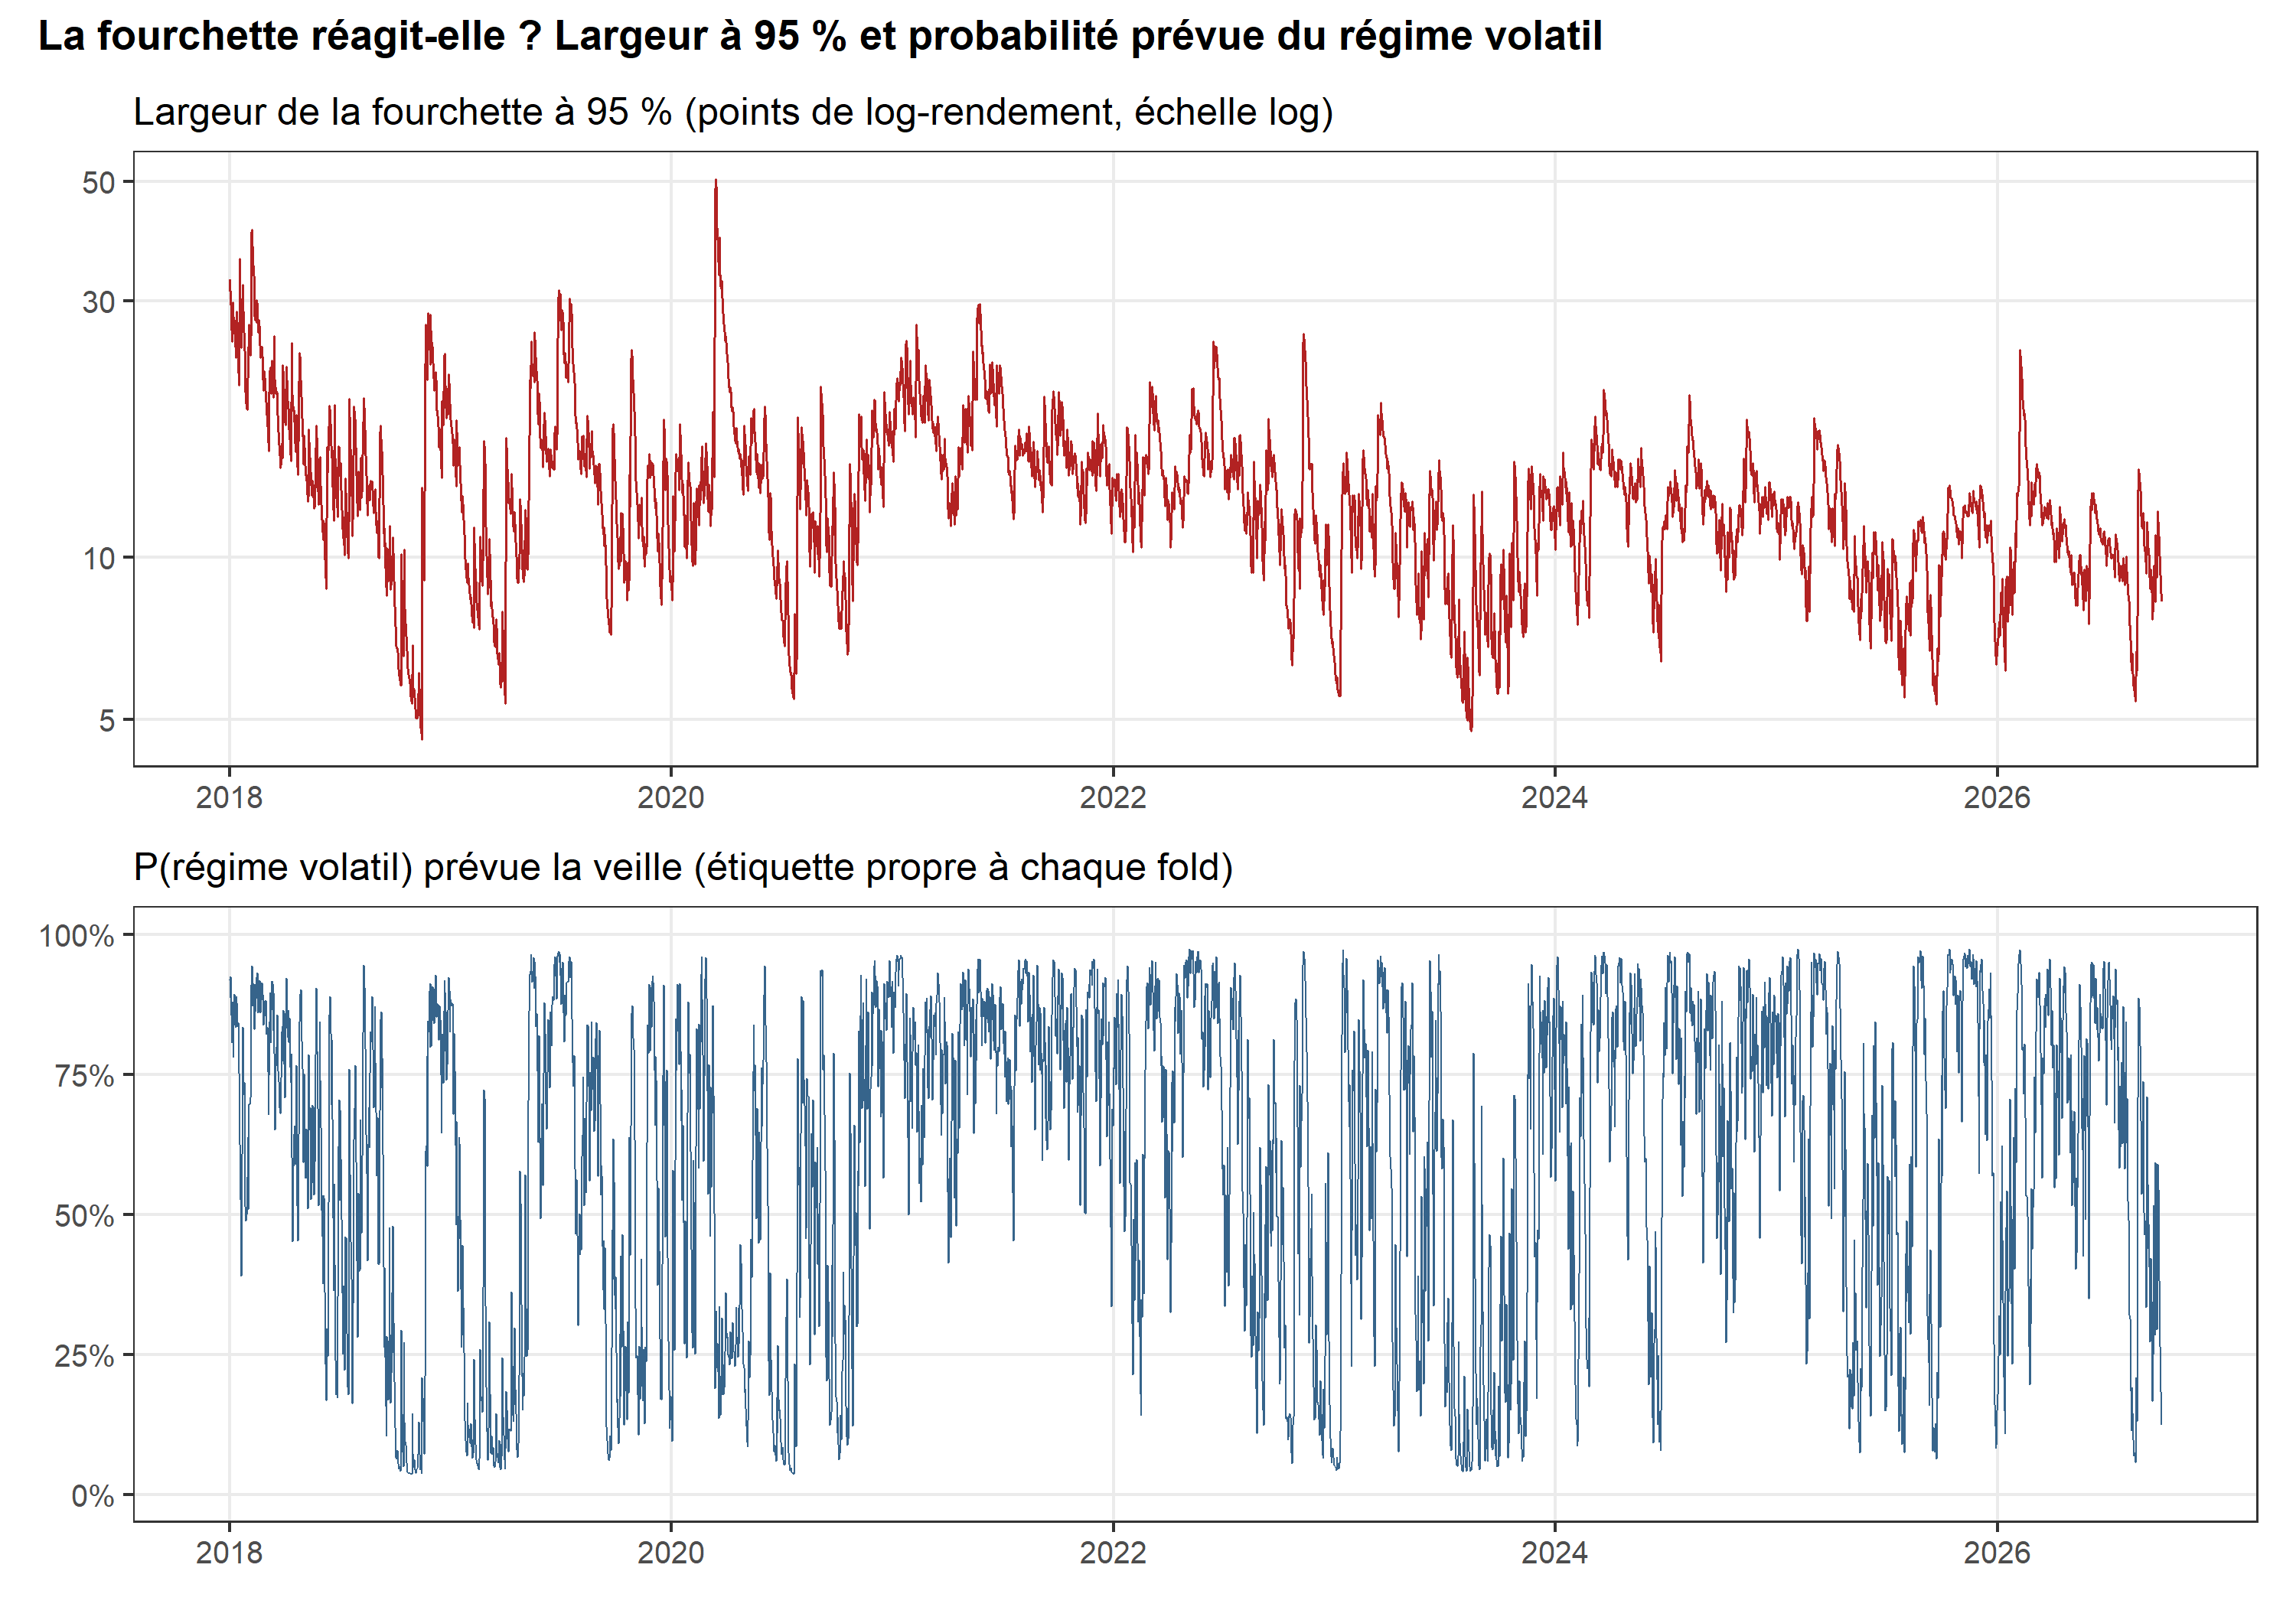
\includegraphics[width=1\linewidth]{15_band_width_and_regime_prob.png}
	\caption{Width of the 95\,\% range (log-return points, log scale) and predicted probability of the volatile regime the day before (label specific to each fold). Figure labels are in French.}
	\label{fig:bt-regime-prob}
\end{figure}


% ═════════════════════════════════════════════════════════════════
\section{Benchmarks: does the regime layer improve the range?}
\label{sec:benchmark}
% ═════════════════════════════════════════════════════════════════

\subsection{Questions and design}

The backtest of section~\ref{sec:backtest} tests the \emph{unconditional} coverage at 95\,\% and the independence of the breaches. It does not say (A) whether the MS-GARCH does better than a simple model, (B) whether the width of the band varies sensibly from one day to the next, (C) by how much the breaches exceed the band, or (D) what happens to direction. This section answers these four questions.

\begin{limitbox}
	\textbf{Status: exploratory.} These checks were not in the design; they do not reopen the verdict of section~\ref{sec:backtest} (PASS). All the comparisons are declared below and no threshold was adjusted after the fact. The $p$-values are indicative.
\end{limitbox}

The comparisons use the same 3,193 days, the same folds, and information up to the previous day only. The reference models are:

\begin{table}[H]
	\centering
	\small
	\caption{The reference models}
	\label{tab:bm-defs}
	\begin{tabular}{lp{8.4cm}}
		\toprule
		Model & Definition \\
		\midrule
		Normal EWMA & RiskMetrics \citep{riskmetrics1996}, $\lambda=0.94$, Normal band \\
		EWMA + FHS & same volatility; quantiles of the empirical distribution of the last 730 standardised returns (filtered historical simulation, \citealt{baronesadesi1999}) \\
		Historical simulation & empirical quantiles of the last 365 returns \\
		Single-regime GARCH-$t$ ($K=1$) & one regime, re-estimated each 1 January ($\alpha+\beta=0.9973$ to $0.9981$ and $\nu=3.20$ to $3.45$ across folds) \\
		\bottomrule
	\end{tabular}
\end{table}

The accuracy of an interval is measured by the \textbf{interval score} \citep{gneitingraftery2007}: the width plus a penalty proportional to the breaches; lower is better. It is compared with the Diebold--Mariano test \citep{dieboldmariano1995} with a Newey--West correction \citep{neweywest1987}; with heavy tails, the $t$ statistic is indicative. Declared comparisons: four for (A), fifteen coverages by tercile for (B1), three tests for (D). The settings of the references ($\lambda=0.94$; windows of 365 and 730 days) were fixed in advance and not optimised.

\subsection{(A) The MS-GARCH against simple models}

\begin{table}[H]
	\centering
	\small
	\caption{95\,\% level: coverage and interval score ($n=3{,}193$; expected breaches: 159.7)}
	\label{tab:bm-95}
	\setlength{\tabcolsep}{4pt}
	\begin{tabular}{lrrrrrrr}
		\toprule
		Model & Br. & Cov. & Kupiec $p$ & Christ.\ $p$ & Width & IS & DM $t$ ($p$) \\
		\midrule
		\textbf{MS-GARCH ($K=2$)} & 156 & $95.11\,\%$ & $0.766$ & $0.610$ & $13.46$ & $\mathbf{18.54}$ & \\
		GARCH-$t$ ($K=1$) & 213 & $93.33\,\%$ & $\mathbf{0.000}$ & $0.299$ & $12.32$ & $18.84$ & $2.19$ ($0.029$) \\
		Normal EWMA & 207 & $93.52\,\%$ & $\mathbf{0.000}$ & $\mathbf{0.000}$ & $12.22$ & $18.85$ & $1.62$ ($0.105$) \\
		EWMA + FHS & 169 & $94.71\,\%$ & $0.452$ & $0.177$ & $13.43$ & $18.98$ & $2.66$ ($0.008$) \\
		Historical simulation & 159 & $95.02\,\%$ & $0.958$ & $\mathbf{0.003}$ & $14.18$ & $19.35$ & $2.35$ ($0.019$) \\
		\bottomrule
	\end{tabular}
\end{table}

\begin{table}[H]
	\centering
	\small
	\caption{99\,\% level (expected breaches: 31.9)}
	\label{tab:bm-99}
	\begin{tabular}{lrrrr}
		\toprule
		Model & Br. & Cov. & Kupiec $p$ & IS \\
		\midrule
		\textbf{MS-GARCH ($K=2$)} & 27 & $99.15\,\%$ & $0.368$ & $\mathbf{29.13}$ \\
		GARCH-$t$ ($K=1$) & 42 & $98.68\,\%$ & $0.088$ & $30.12$ \\
		Normal EWMA & 109 & $96.59\,\%$ & $\mathbf{0.000}$ & $33.92$ \\
		EWMA + FHS & 42 & $98.68\,\%$ & $0.088$ & $31.57$ \\
		Historical simulation & 40 & $98.75\,\%$ & $0.167$ & $29.50$ \\
		\bottomrule
	\end{tabular}
\end{table}

DM: $t>0$ means that the model is worse than the MS-GARCH.

\textbf{Reading.}
\begin{itemize}
	\item \textbf{The MS-GARCH has the best interval score at 95 and 99\,\%, but the margin is small at 95\,\%}: $1.6\,\%$ against the single-regime GARCH-$t$ and the Normal EWMA, $2.3\,\%$ against EWMA + FHS, $4.2\,\%$ against historical simulation. At 99\,\% the margin runs from $1.3\,\%$ (historical simulation) to $14\,\%$ (Normal EWMA).
	\item \textbf{Statistical strength.} With four comparisons (Bonferroni threshold $0.0125$), only the gap with EWMA + FHS ($p=0.008$) holds. The $p$-values of $0.029$ ($K=1$) and $0.019$ (historical simulation) do not survive the correction.
	\item \textbf{The success criterion of section~\ref{sec:backtest} does not discriminate.} EWMA + FHS passes it too (Kupiec $p=0.452$; Christoffersen $p=0.177$), with a nearly identical band width ($13.43$ against $13.46$). Historical simulation passes Kupiec but fails independence ($p=0.003$): its breaches cluster.
	\item \textbf{What the simple references miss.} The single-regime GARCH-$t$ and the Normal EWMA under-cover at 95\,\% ($93.3\,\%$ and $93.5\,\%$, $p=0.000$). The Normal EWMA misses the extremes at 99\,\% massively (109 breaches for 31.9 expected): heavy tails matter, and the Normal is not defensible here.
	\item \textbf{The own contribution of the MS-GARCH}, at the end of (A): a better calibration than the single-regime GARCH-$t$ ($95.1\,\%$ against $93.3\,\%$) and, at 99\,\%, a coverage that is not rejected (Kupiec $p=0.368$) where EWMA + FHS and $K=1$ stand at $p=0.088$.
\end{itemize}

\begin{limitbox}
	\textbf{The honest answer to ``does the pipeline transfer?''} The coverage transfers (section~\ref{sec:backtest}), but a simple, heavy-tailed model obtains it as well: the filtered historical simulation passes the same two tests with a band of the same width. The regime layer improves the interval score by a small margin, solidly against one reference only. This is a result on the \emph{added value of the regime layer}, not a failure of the pipeline: the same conclusion was reached on EUR/USD, where the regime layer was not shown to improve the range either \citep{ZEWU2026fx}.
\end{limitbox}

\subsection{(B1) Coverage by tercile of band width}

\begin{table}[H]
	\centering
	\small
	\caption{95\,\% coverage by tercile of band width (Kupiec $p$ in parentheses, uncorrected)}
	\label{tab:bm-terciles}
	\begin{tabular}{lccc}
		\toprule
		Model & Narrow & Medium & Wide \\
		\midrule
		\textbf{MS-GARCH ($K=2$)} & $94.37\,\%$ ($0.35$) & $94.64\,\%$ ($0.60$) & $96.33\,\%$ ($0.036$) \\
		GARCH-$t$ ($K=1$) & $91.92\,\%$ ($0.000$) & $92.48\,\%$ ($0.000$) & $95.58\,\%$ ($0.37$) \\
		Normal EWMA & $90.70\,\%$ ($0.000$) & $94.45\,\%$ ($0.42$) & $95.39\,\%$ ($0.55$) \\
		EWMA + FHS & $92.39\,\%$ ($0.000$) & $94.74\,\%$ ($0.70$) & $96.99\,\%$ ($0.001$) \\
		Historical simulation & $94.19\,\%$ ($0.24$) & $94.26\,\%$ ($0.28$) & $96.65\,\%$ ($0.009$) \\
		\bottomrule
	\end{tabular}
\end{table}

All models share the same profile: the coverage rises with the width (narrow bands slightly too tight, wide bands slightly too cautious). \textbf{The MS-GARCH is the most uniform}: no rejection in the first two terciles, and its only gap ($96.33\,\%$; 39 breaches for 53 expected) is on the cautious side. The $p$-values are not corrected over 15 tests and are indicative.

\subsection{(B2) Does the width follow the size of the day's move?}

\begin{table}[H]
	\centering
	\caption{Regression of $|{\rm return}|$ on the half-width of the 95\,\% band}
	\label{tab:bm-mz}
	\begin{tabular}{lrrr}
		\toprule
		Model & Slope & $t$ (HAC) & $R^2$ \\
		\midrule
		MS-GARCH ($K=2$) & $0.297$ & $15.7$ & $0.085$ \\
		GARCH-$t$ ($K=1$) & $0.271$ & $11.2$ & $0.083$ \\
		Normal EWMA & $0.283$ & $11.9$ & $0.088$ \\
		EWMA + FHS & $0.257$ & $12.5$ & $0.084$ \\
		Historical simulation & $0.234$ & $6.8$ & $0.031$ \\
		\bottomrule
	\end{tabular}
\end{table}

The width of the MS-GARCH band does follow the size of the day's move ($t=15.7$; a constant-width band would give $R^2=0$). But \textbf{the ranking of risky days is not better than that of a simple EWMA} ($R^2$ of $0.085$ against $0.088$); only historical simulation, which adapts slowly, drops ($0.031$). The absolute $R^2$ is low because $|{\rm return}|$ is a very noisy indicator of the day's volatility: only the comparison between models is informative.

\textbf{Consequence:} the contribution of the MS-GARCH is not to spot risky days better; it lies in the \emph{shape} of the distribution (the calibration of the tails), not in the \emph{ranking}.

\subsection{(C) Size of the breaches}

\begin{table}[H]
	\centering
	\footnotesize
	\caption{Size of the MS-GARCH breaches (in points of return; hw $=$ half-width of the band)}
	\label{tab:bm-size}
	\setlength{\tabcolsep}{3pt}
	\begin{tabular}{lrrrrrrrr}
		\toprule
		Level & Br. & Mean & Med. & P90 & Max & Mean/hw & Max/hw & Days $>1$ hw \\
		\midrule
		95\,\% & 156 & $2.60$ & $1.45$ & $5.74$ & $39.40$ & $0.47$ & $5.57$ & 17 \\
		99\,\% & 27 & $3.69$ & $1.97$ & $5.52$ & $34.76$ & $0.40$ & $2.92$ & 3 \\
		\bottomrule
	\end{tabular}
\end{table}

Most breaches are \textbf{marginal} (median of $1.45$ points at 95\,\%), but the distribution of sizes has a heavy tail: 17 breaches out of 156 ($11\,\%$) exceed the bound by more than a half-width. The maximum, on 2020-03-12 ($-46.5\,\%$ in log-return), lies $5.6$ half-widths beyond the 95\,\% bound and $2.9$ beyond the 99\,\% bound.

\begin{figure}[H]
	\centering
	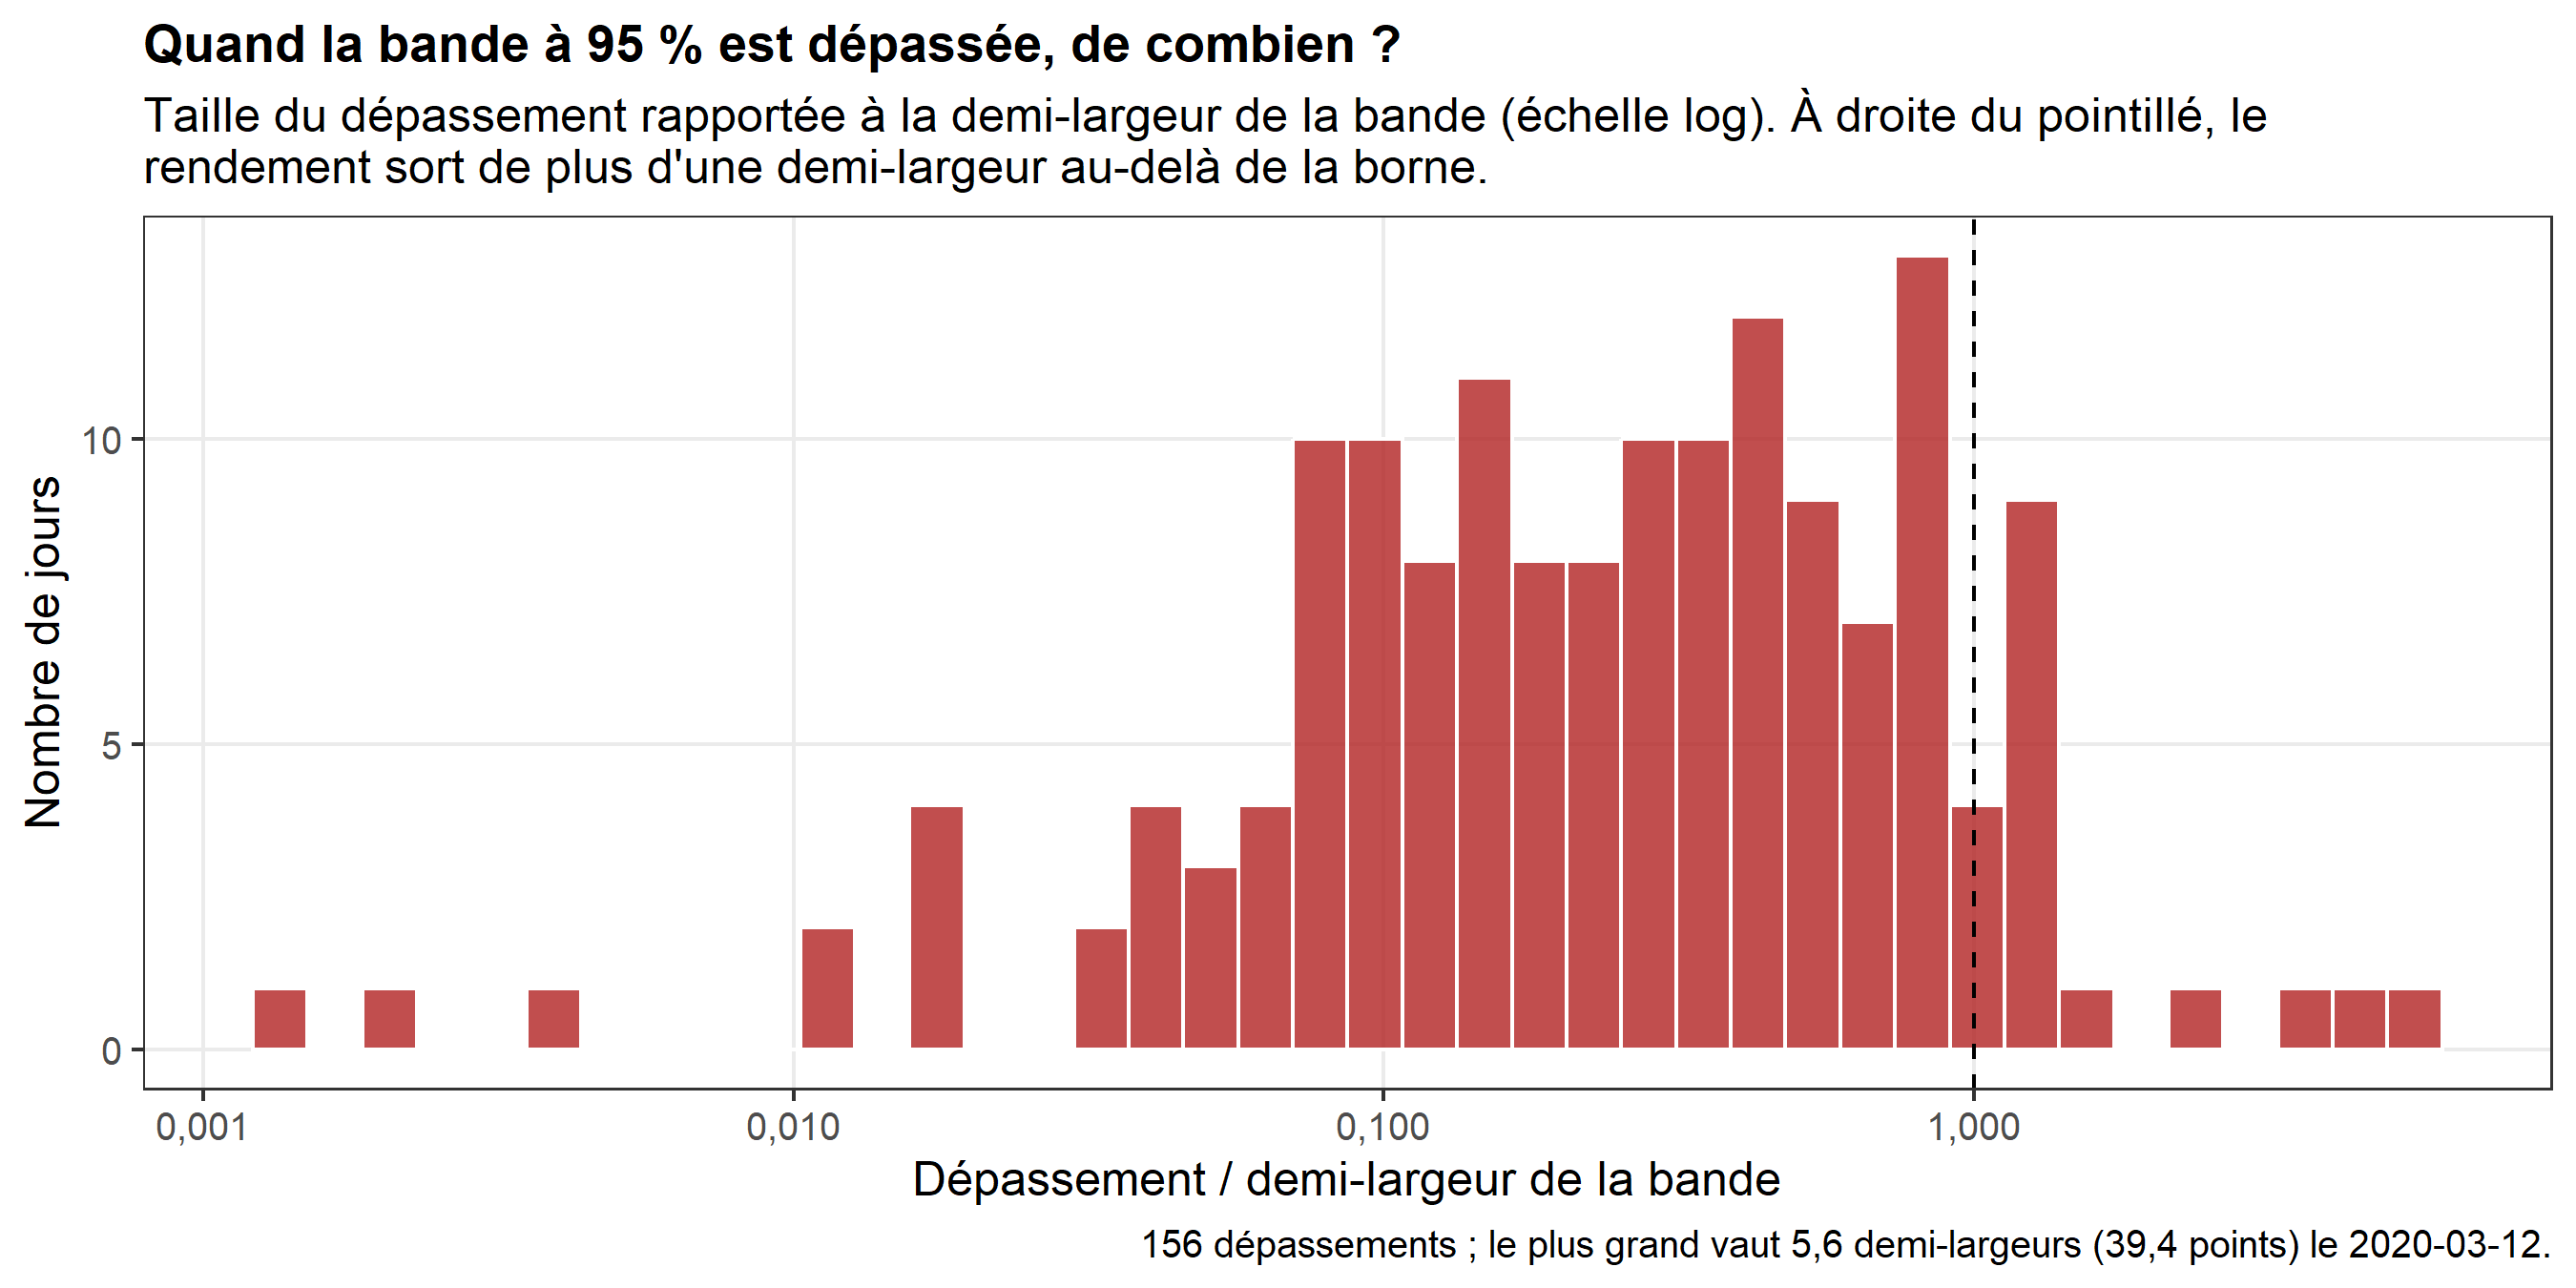
\includegraphics[width=1\linewidth]{D7_breach_size.png}
	\caption{Size of the 95\,\% breaches relative to the half-width of the band (log scale). To the right of the dashed line, the return exceeds the bound by more than one half-width. The largest breach is $5.6$ half-widths (39.4 points), on 2020-03-12. Figure labels are in French.}
	\label{fig:bm-breach-size}
\end{figure}

\subsection{(D) Direction}

\begin{table}[H]
	\centering
	\small
	\caption{Three simple direction tests (Bonferroni threshold for three tests: $0.0167$)}
	\label{tab:bm-direction}
	\begin{tabular}{p{5cm}p{5.3cm}p{3.1cm}}
		\toprule
		Test & Result & Significant? \\
		\midrule
		Ljung--Box on returns, lag 10 / lag 20 & $p=0.029$ / $0.075$ & no \\
		Sign persistence at one day & $2{,}111/4{,}391=48.1\,\%$; binomial $p=0.011$ & \textbf{yes} \\
		20-day trend $\to$ sign of the next day (backtest days) & $1{,}616/3{,}193=50.6\,\%$; $p=0.50$ & no \\
		\emph{Witness: Ljung--Box on $|{\rm returns}|$} & $p\approx0$ (lags 10 and 20) & massive volatility clustering \\
		\bottomrule
	\end{tabular}
\end{table}

The share of up days is $50.9\,\%$ and the mean return over the backtest days is $0.056\,\%$ per day (a realised drift, not a forecast). Pairs involving the single zero return are excluded from the sign-persistence count.

\textbf{Reading.} Volatility is predictable and direction hardly: the witness rejects the absence of dependence massively, the returns themselves barely. One signal stands out: after an up day the next day is a little more often down (and conversely), with $48.1\,\%$ of same-sign days against $50\,\%$. It crosses the Bonferroni threshold ($p=0.011<0.0167$) but the \textbf{gap is $1.9$ points}, before any transaction cost. The sign test is robust to heavy tails (it does not depend on moments); the Ljung--Box test is not ($\nu\approx3$: infinite fourth moment).

\begin{econbox}[Statistically significant is not economically exploitable]
	A gap of under two points between $48.1\,\%$ and $50\,\%$ is easily absorbed by fees, spreads and slippage. No test net of costs was run, so this result justifies no strategy. It is consistent with a very liquid and closely watched market, where direction is not predictable from the price history alone. But only three simple signals were tried: this is not a proof of unpredictability.
\end{econbox}

\subsection{What to retain}

\begin{enumerate}
	\item The success criterion is passed, but \textbf{it is weakly discriminating}: a simple model (EWMA + FHS) passes it too.
	\item The MS-GARCH has the best interval score of the five models, by a \emph{small} margin at 95\,\% and solidly only against EWMA + FHS.
	\item Its contribution is the \textbf{calibration of the tails and the uniformity of the coverage}, not the ranking of risky days.
	\item The breaches are mostly marginal; the tail of their sizes is heavy and dominated by 2020-03-12.
	\item Direction: nothing exploitable with the signals tested.
\end{enumerate}

\begin{econbox}[What this means for a practitioner]
	A practitioner can obtain most of the result with a much simpler tool. If the value of the MS-GARCH is said to lie in its regime reading, sections~\ref{sec:msgarch} and~\ref{sec:backtest} qualify that claim strongly: the labels are relative to each re-estimation, 42.6\,\% of the days are ambiguous, and the regime probability does not rank the risky days better than an EWMA. What the evidence supports is narrower: a well-calibrated range with heavy-tailed quantiles, to which the regime layer adds a small and fragile improvement.
\end{econbox}

\subsection{Limits}

\begin{itemize}
	\item \textbf{Exploratory}: never planned in the design, not corrected for multiple comparisons beyond what is stated; the $p$-values are indicative.
	\item The settings of the references are fixed in advance and not optimised ($\lambda=0.94$; windows of 365 and 730 days): another setting could change the gap.
	\item The interval score is tested at 95\,\% only.
	\item One run, one asset.
\end{itemize}


% ═════════════════════════════════════════════════════════════════
\section{General conclusion}
\label{sec:conclusion}
% ═════════════════════════════════════════════════════════════════

\subsection{The answer to the question}

The question was whether a one-day price range can be built for Bitcoin and be calibrated out of sample, and what an analyst can use it for. The answer has two parts of unequal strength.

\textbf{At the 95\,\% level, the range is calibrated.} Over 3,193 out-of-sample forecasts (2018--2026), the coverage is $95.11\,\%$ (Wilson interval $94.3\,\%$ to $95.8\,\%$), with 156 breaches for 159.7 expected, Kupiec $p=0.766$ and Christoffersen $p=0.610$. During the shock of March 2020, with the model frozen at the end of 2019, the coverage did not collapse ($95.87\,\%$ over 121 days, a qualitative test). The study was declared successful if the coverage criterion was passed and the result was not classified as an ``era''; both conditions hold: the coverage criterion is passed and the rule finds 51 switches and a longest volatile block of $15.4\,\%$ of the sample.

\textbf{What that does not establish is considerable.} The criterion is weakly discriminating: a filtered historical simulation passes it too, with a band of the same width. The MS-GARCH has the best interval score of the five models, but by a small margin at 95\,\% ($1.6$ to $4.2\,\%$), and only the gap with that one reference survives a multiple-comparison correction. Its contribution lies in the calibration of the tails and the uniformity of the coverage, not in the ranking of risky days.

\subsection{What the study shows}

\begin{itemize}
	\item \textbf{The chain runs on Bitcoin and produces interpretable diagnostics}, at the price of three declared adaptations (a multi-start fit, an exact fallback when \texttt{Risk()} saturates, a cautious reading of the regime labels).
	\item \textbf{The regimes are persistent and alternate} (expected durations of about 73 and 36 days); the near-unit persistence is not removed by a single level shift between the two halves of the sample, nor by allowing two regimes.
	\item \textbf{The tails are very heavy but their index is not identified}: $\nu$ is $3.18$ in the single-regime GARCH, between $2.3$ and $4$ by regime, and the Hill estimator has no plateau. No single value of $\nu$ should be quoted as a constant of the market.
	\item \textbf{The Normal is not defensible}: the Normal EWMA misses the extremes at 99\,\% (109 breaches for 31.9 expected).
	\item \textbf{Direction is not exploitable} with the three simple signals tested.
\end{itemize}

\subsection{What the study does not show}

\begin{itemize}
	\item \textbf{The size of the extreme losses.} The coverage counts breaches, not their magnitude: on 2020-03-12 the log return of $-46.5\,\%$ (a price fall of $37.2\,\%$) was $6.6$ times its lower bound, and 17 breaches out of 156 exceed the bound by more than a half-width. No 95\,\% band contains such a day. The 99\,\% coverage ($99.15\,\%$, 27 breaches) is reported without pass/fail and must not be presented as validated in the same way as the 95\,\%.
	\item \textbf{That the MS-GARCH is necessary}, or that its regime reading is meaningful in itself: the labels are relative to each re-estimation, 42.6\,\% of the days are ambiguous, and the regime probability does not rank the risky days better than an EWMA.
	\item \textbf{A structural reading of the persistence}: the explanation by unmodelled breaks is not supported by the split-sample test, but that test is corroborating, not decisive, and multiple breaks or long memory remain possible.
	\item \textbf{Causes}, the value of the asset, platform, counterparty and regulatory risks, intraday amplitude, or horizons longer than one day.
\end{itemize}

\begin{econbox}[Reading for an analyst of the Bitcoin market]
	The model can serve as a \textbf{gauge of the size of an ordinary day}: a one-day range of about $\pm4\,\%$ at the end of the sample, whose width moves with the volatility forecast and whose coverage is calibrated at 95\,\%. It cannot serve as a forecast of the price, of its direction, of the size of extreme moves, or as an explanation of why the risk changes. Because the range is built from past volatility, it widens after a shock (from $14$ to about $50$ points of log return around 12 March 2020), not before. A practitioner who needs only the calibrated band can obtain most of it with a simpler tool; the evidence for the added value of the regime layer is small and fragile. The contrast with EUR/USD is a main result of the study: the method works statistically on both assets, but the economic reading differs deeply (maximal persistence, heavier tails, a volatile regime that is the majority state), and for an asset with no anchor these may be real properties rather than artefacts.
\end{econbox}

\subsection{Limits}

\begin{itemize}
	\item One asset, one split into folds, one run; the number of regimes was settled on EUR/USD, not on Bitcoin.
	\item A single data source (\texttt{yfinance}) without a second-provider cross-check, and a closing price that is a convention (midnight UTC).
	\item The persistence sits on the boundary and $\nu\le4$ in both regimes: the standard errors and the tests on squared residuals rest on assumptions that do not hold exactly there.
	\item A residual dependence in $|z_t|$ that the single-regime GARCH does not capture; the global optimality of the MS-GARCH fit is supported by repetition, not demonstrated.
	\item The success criterion has a calibration power of about $\pm0.76$ point and a false-rejection risk of about $10\,\%$ from two tests at $5\,\%$; the exploratory sections are not corrected for multiple comparisons.
	\item The observations made after the fact (absence of 99\,\% breaches in 2024--2025, drift towards conservatism) are leads, not results.
\end{itemize}

\subsection{Further work}

The following questions arose from the study; they are to be tested, not presumed.
\begin{itemize}
	\item Why does the two-regime model separate scale from tails rather than calm from crisis? A model with $K\ge3$ or another definition of regimes could be tried.
	\item Why were there no 99\,\% breaches in 2024--2025, and would a rolling estimation window reduce the drift towards conservatism better than an expanding one?
	\item Multiple breaks or long memory, against persistence at the boundary; and the residual dependence in $|z_t|$.
	\item Direction, with controls specific to Bitcoin (only three simple signals were tested here).
	\item Why the ranking of risky days is not better than that of a simple EWMA.
	\item A second data source, and horizons longer than one day by multi-step simulation.
\end{itemize}

\subsection{Transparency}

The record of what was fixed before and after the data (Table~\ref{tab:status}) is part of the result: a reader can see which conclusions rest on a pre-specified test and which on an observation made after the fact. The corrections made along the way are logged in Appendix~\ref{sec:app-log}.



\newpage
\addcontentsline{toc}{section}{References}
\begin{thebibliography}{99}
	\bibitem[Zewu(2026)]{ZEWU2026fx}
	Armand Zewu,.~Y.~I. (2026). Quantitative Modeling of EUR/USD Exchange Rate Volatility. \textit{SSRN Working Paper} No.~7532760.

	\bibitem[Ardia et al.(2018)]{ardia2018}
	Ardia, D., Bluteau, K., Boudt, K., \& Catania, L. (2018). Forecasting risk with Markov-switching GARCH models: A large-scale performance study. \textit{International Journal of Forecasting}, 34(4), 733--747.

	\bibitem[Ardia et al.(2019)]{ardia2019}
	Ardia, D., Bluteau, K., Boudt, K., Catania, L., \& Trottier, D.-A.
	(2019). Markov-Switching GARCH Models in R: The MSGARCH Package.
	\textit{Journal of Statistical Software}, 91(4), 1--38.

	\bibitem[Barone-Adesi et al.(1999)]{baronesadesi1999}
	Barone-Adesi, G., Giannopoulos, K., \& Vosper, L. (1999). VaR without Correlations for Portfolios of Derivative Securities. \textit{Journal of Futures Markets}, 19(5), 583--602.

	\bibitem[Bollerslev(1986)]{bollerslev1986}
	Bollerslev, T. (1986). Generalized Autoregressive Conditional Heteroskedasticity. \textit{Journal of Econometrics}, 31(3), 307--327.

	\bibitem[Bollerslev(1987)]{bollerslev1987}
	Bollerslev, T. (1987). A Conditionally Heteroskedastic Time Series Model for Speculative Prices and Rates of Return. \textit{Review of Economics and Statistics}, 69(3), 542--547.

	\bibitem[Chow(1960)]{chow1960}
	Chow, G.~C. (1960). Tests of Equality Between Sets of Coefficients in Two Linear Regressions. \textit{Econometrica}, 28(3), 591--605.

	\bibitem[Christoffersen(1998)]{christoffersen1998}
	Christoffersen, P.~F. (1998). Evaluating Interval Forecasts. \textit{International Economic Review}, 39(4), 841--862.

	\bibitem[Diebold and Mariano(1995)]{dieboldmariano1995}
	Diebold, F.~X., \& Mariano, R.~S. (1995). Comparing Predictive Accuracy. \textit{Journal of Business \& Economic Statistics}, 13(3), 253--263.

	\bibitem[Engle(1982)]{engle1982}
	Engle, R.~F. (1982). Autoregressive Conditional Heteroscedasticity with Estimates of the Variance of United Kingdom Inflation. \textit{Econometrica}, 50(4), 987--1007.

	\bibitem[Garcia(1998)]{garcia1998}
	Garcia, R. (1998). Asymptotic Null Distribution of the Likelihood Ratio Test in Markov Switching Models. \textit{International Economic Review}, 39(3), 763--788.

	\bibitem[Gneiting and Raftery(2007)]{gneitingraftery2007}
	Gneiting, T., \& Raftery, A.~E. (2007). Strictly Proper Scoring Rules, Prediction, and Estimation. \textit{Journal of the American Statistical Association}, 102(477), 359--378.

	\bibitem[Gray(1996)]{gray1996}
	Gray, S.~F. (1996). Modeling the Conditional Distribution of Interest
	Rates as a Regime-Switching Process. \textit{Journal of Financial
		Economics}, 42(1), 27--62.

	\bibitem[Haas et al.(2004)]{haasmittnikpaolella2004}
	Haas, M., Mittnik, S., \& Paolella, M.~S. (2004a). A New Approach to
	Markov-Switching GARCH Models. \textit{Journal of Financial
		Econometrics}, 2(4), 493--530.

	\bibitem[Hamilton and Susmel(1994)]{hamiltonsusmel1994}
	Hamilton, J.~D., \& Susmel, R. (1994). Autoregressive Conditional
	Heteroskedasticity and Changes in Regime. \textit{Journal of
		Econometrics}, 64(1--2), 307--333.

	\bibitem[Hansen(1992)]{hansen1992}
	Hansen, B.~E. (1992). The Likelihood Ratio Test under Nonstandard Conditions: Testing the Markov Switching Model of GNP. \textit{Journal of Applied Econometrics}, 7(S1), S61--S82.

	\bibitem[J.P.~Morgan/Reuters(1996)]{riskmetrics1996}
	J.P.~Morgan/Reuters (1996). \textit{RiskMetrics --- Technical Document}, 4th edition. New York: J.P.~Morgan.

	\bibitem[Kupiec(1995)]{kupiec1995}
	Kupiec, P.~H. (1995). Techniques for Verifying the Accuracy of Risk Measurement Models. \textit{Journal of Derivatives}, 3(2), 73--84.

	\bibitem[Lamoureux and Lastrapes(1990)]{lamoureuxlastrapes1990}
	Lamoureux, C.~G., \& Lastrapes, W.~D. (1990). Persistence in Variance, Structural Change, and the GARCH Model. \textit{Journal of Business \& Economic Statistics}, 8(2), 225--234.
	
	% UNVERIFIED (added for the BTC paper; standard citations, to check before submission)

	\bibitem[Newey and West(1987)]{neweywest1987}
	Newey, W.~K., \& West, K.~D. (1987). A Simple, Positive Semi-Definite, Heteroskedasticity and Autocorrelation Consistent Covariance Matrix. \textit{Econometrica}, 55(3), 703--708.
	
	% UNVERIFIED

	\bibitem[West(1996)]{west1996}
	West, K.~D. (1996). Asymptotic Inference about Predictive Ability.
	\textit{Econometrica}, 64(5), 1067--1084.
	
	
	% ---- References added in v2. VERIFIED = checked against the publisher or an index; UNVERIFIED = standard citation, to check before submission.
	% VERIFIED

\end{thebibliography}

% ═════════════════════════════════════════════════════════════════
\appendix
\section{Supplementary figures}
\label{sec:app-figs}
% ═════════════════════════════════════════════════════════════════

\subsection{Smoothed and filtered probability, March 2020}

\begin{figure}[H]
	\centering
	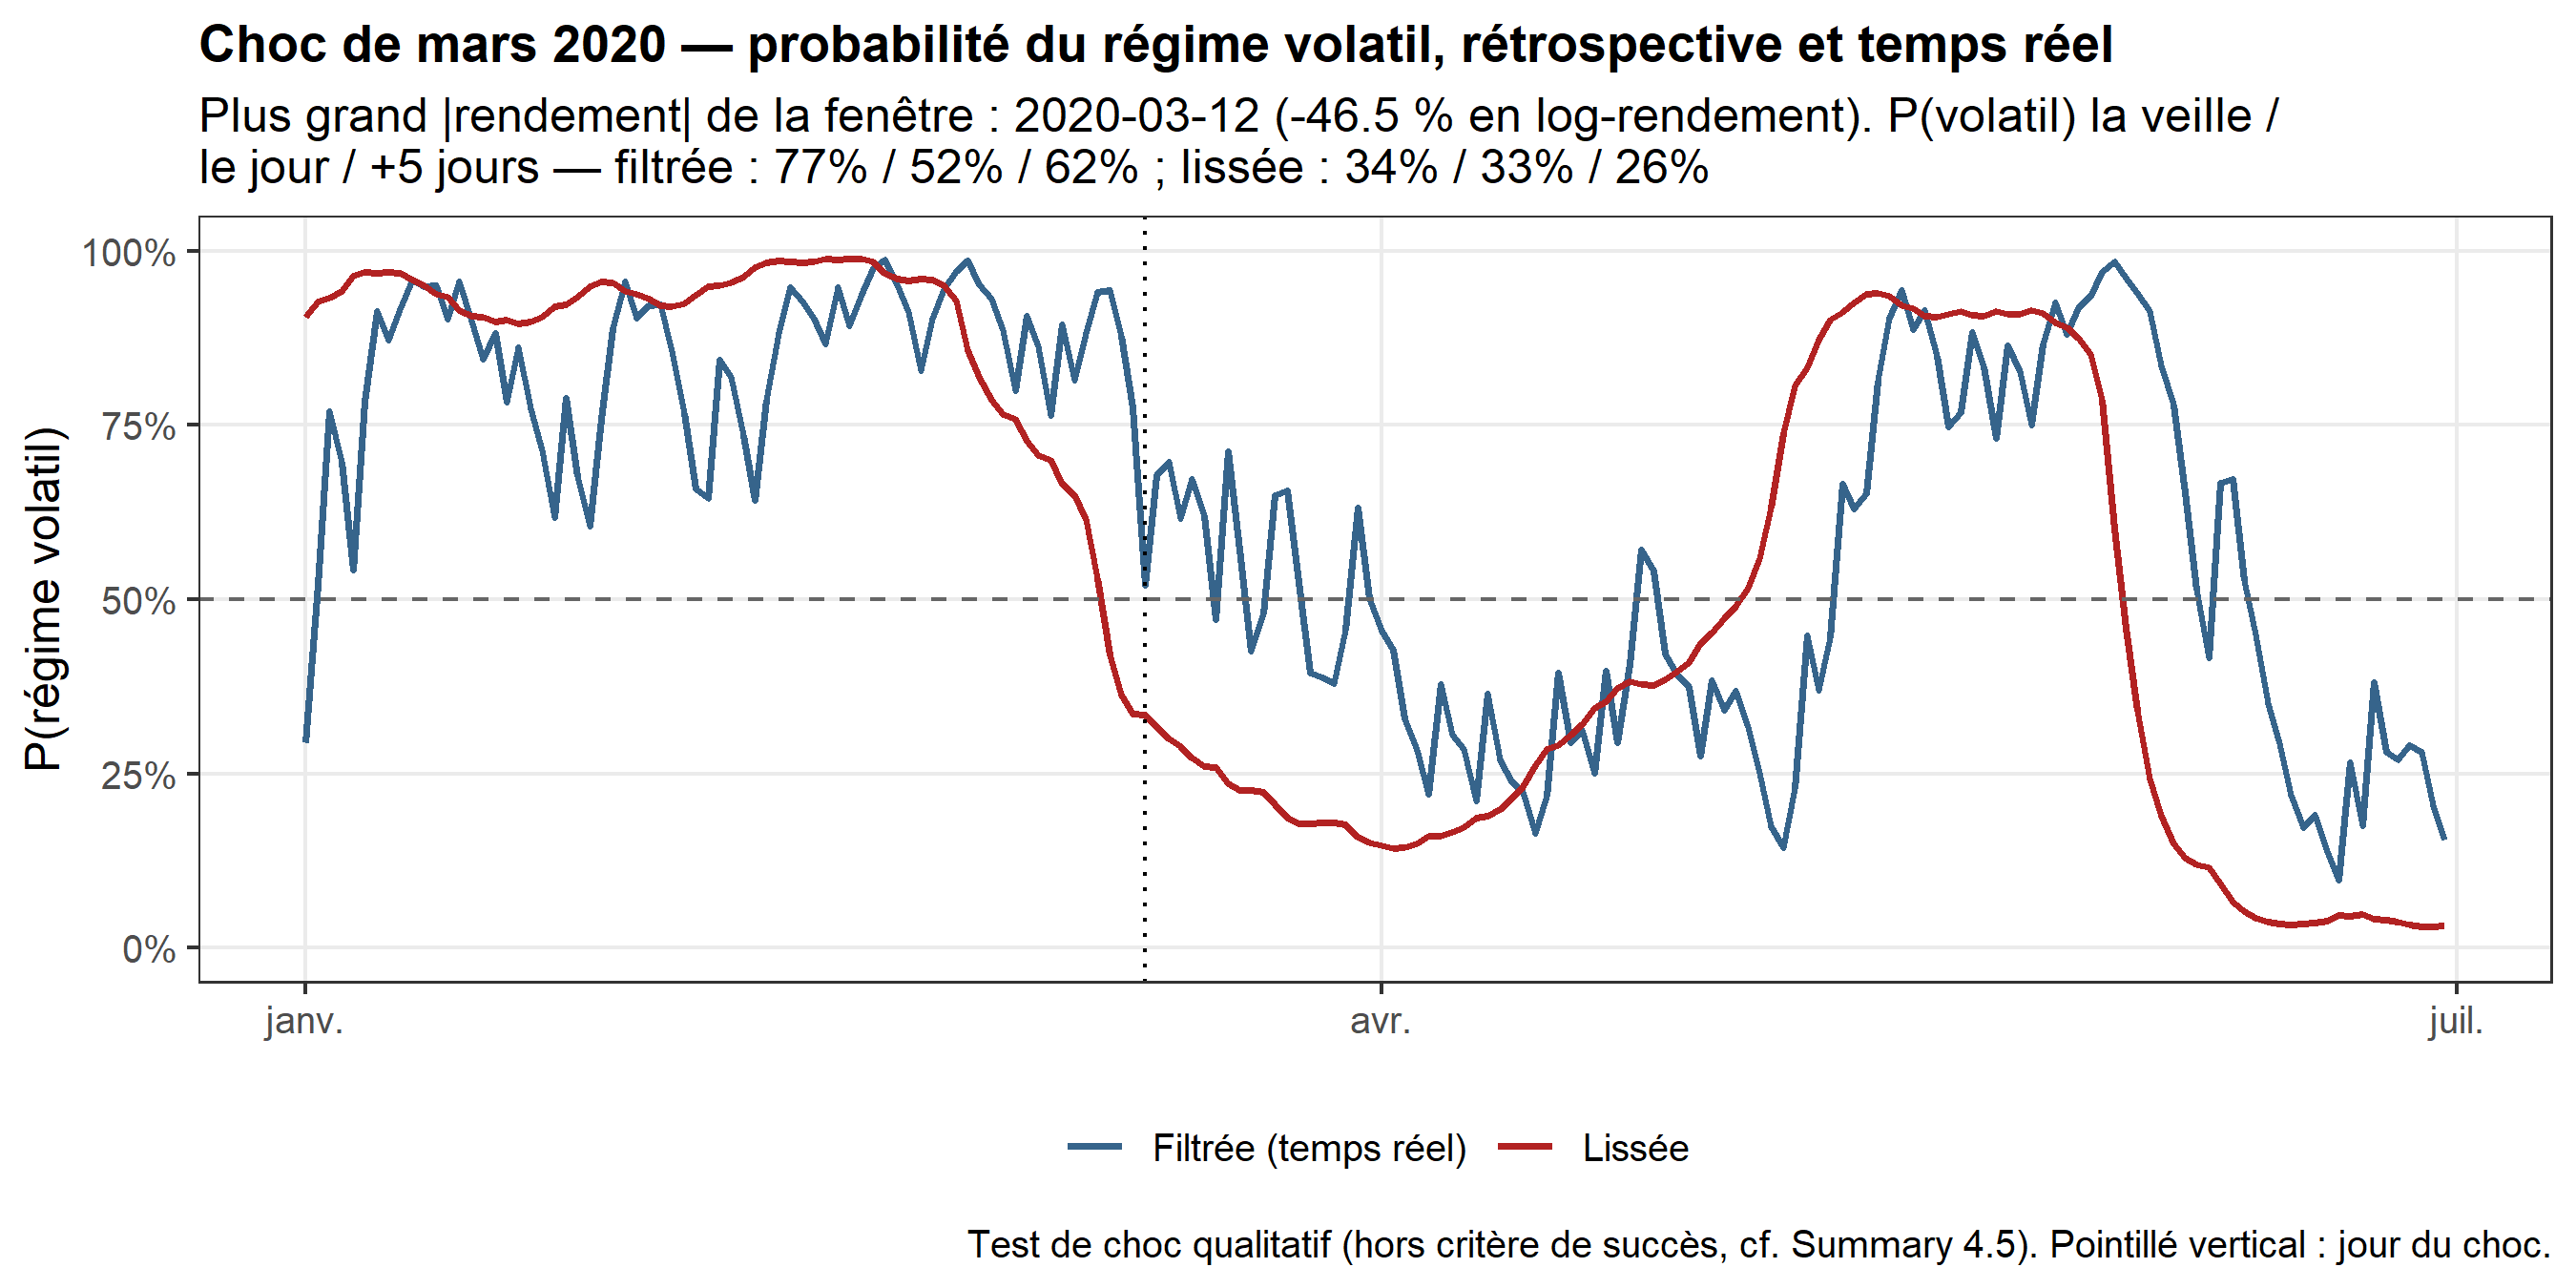
\includegraphics[width=1\linewidth]{02_shock_2020_smoothed_vs_filtered.png}
	\caption{Probability of the volatile regime around the shock of March 2020 (full-sample estimation): filtered (real time) and smoothed (\emph{ex post}). The dotted line marks 2020-03-12. On that day the filtered probability is $0.521$ (it was $0.775$ the day before) and the smoothed probability $0.334$: the largest shock of the sample is attributed to the calm regime. The subtitle of the figure gives these probabilities the day before, on the day and five days after, rounded to the percent. Figure labels are in French.}
	\label{fig:app-shock-prob}
\end{figure}

\subsection{Share of volatile days by year}

\begin{figure}[H]
	\centering
	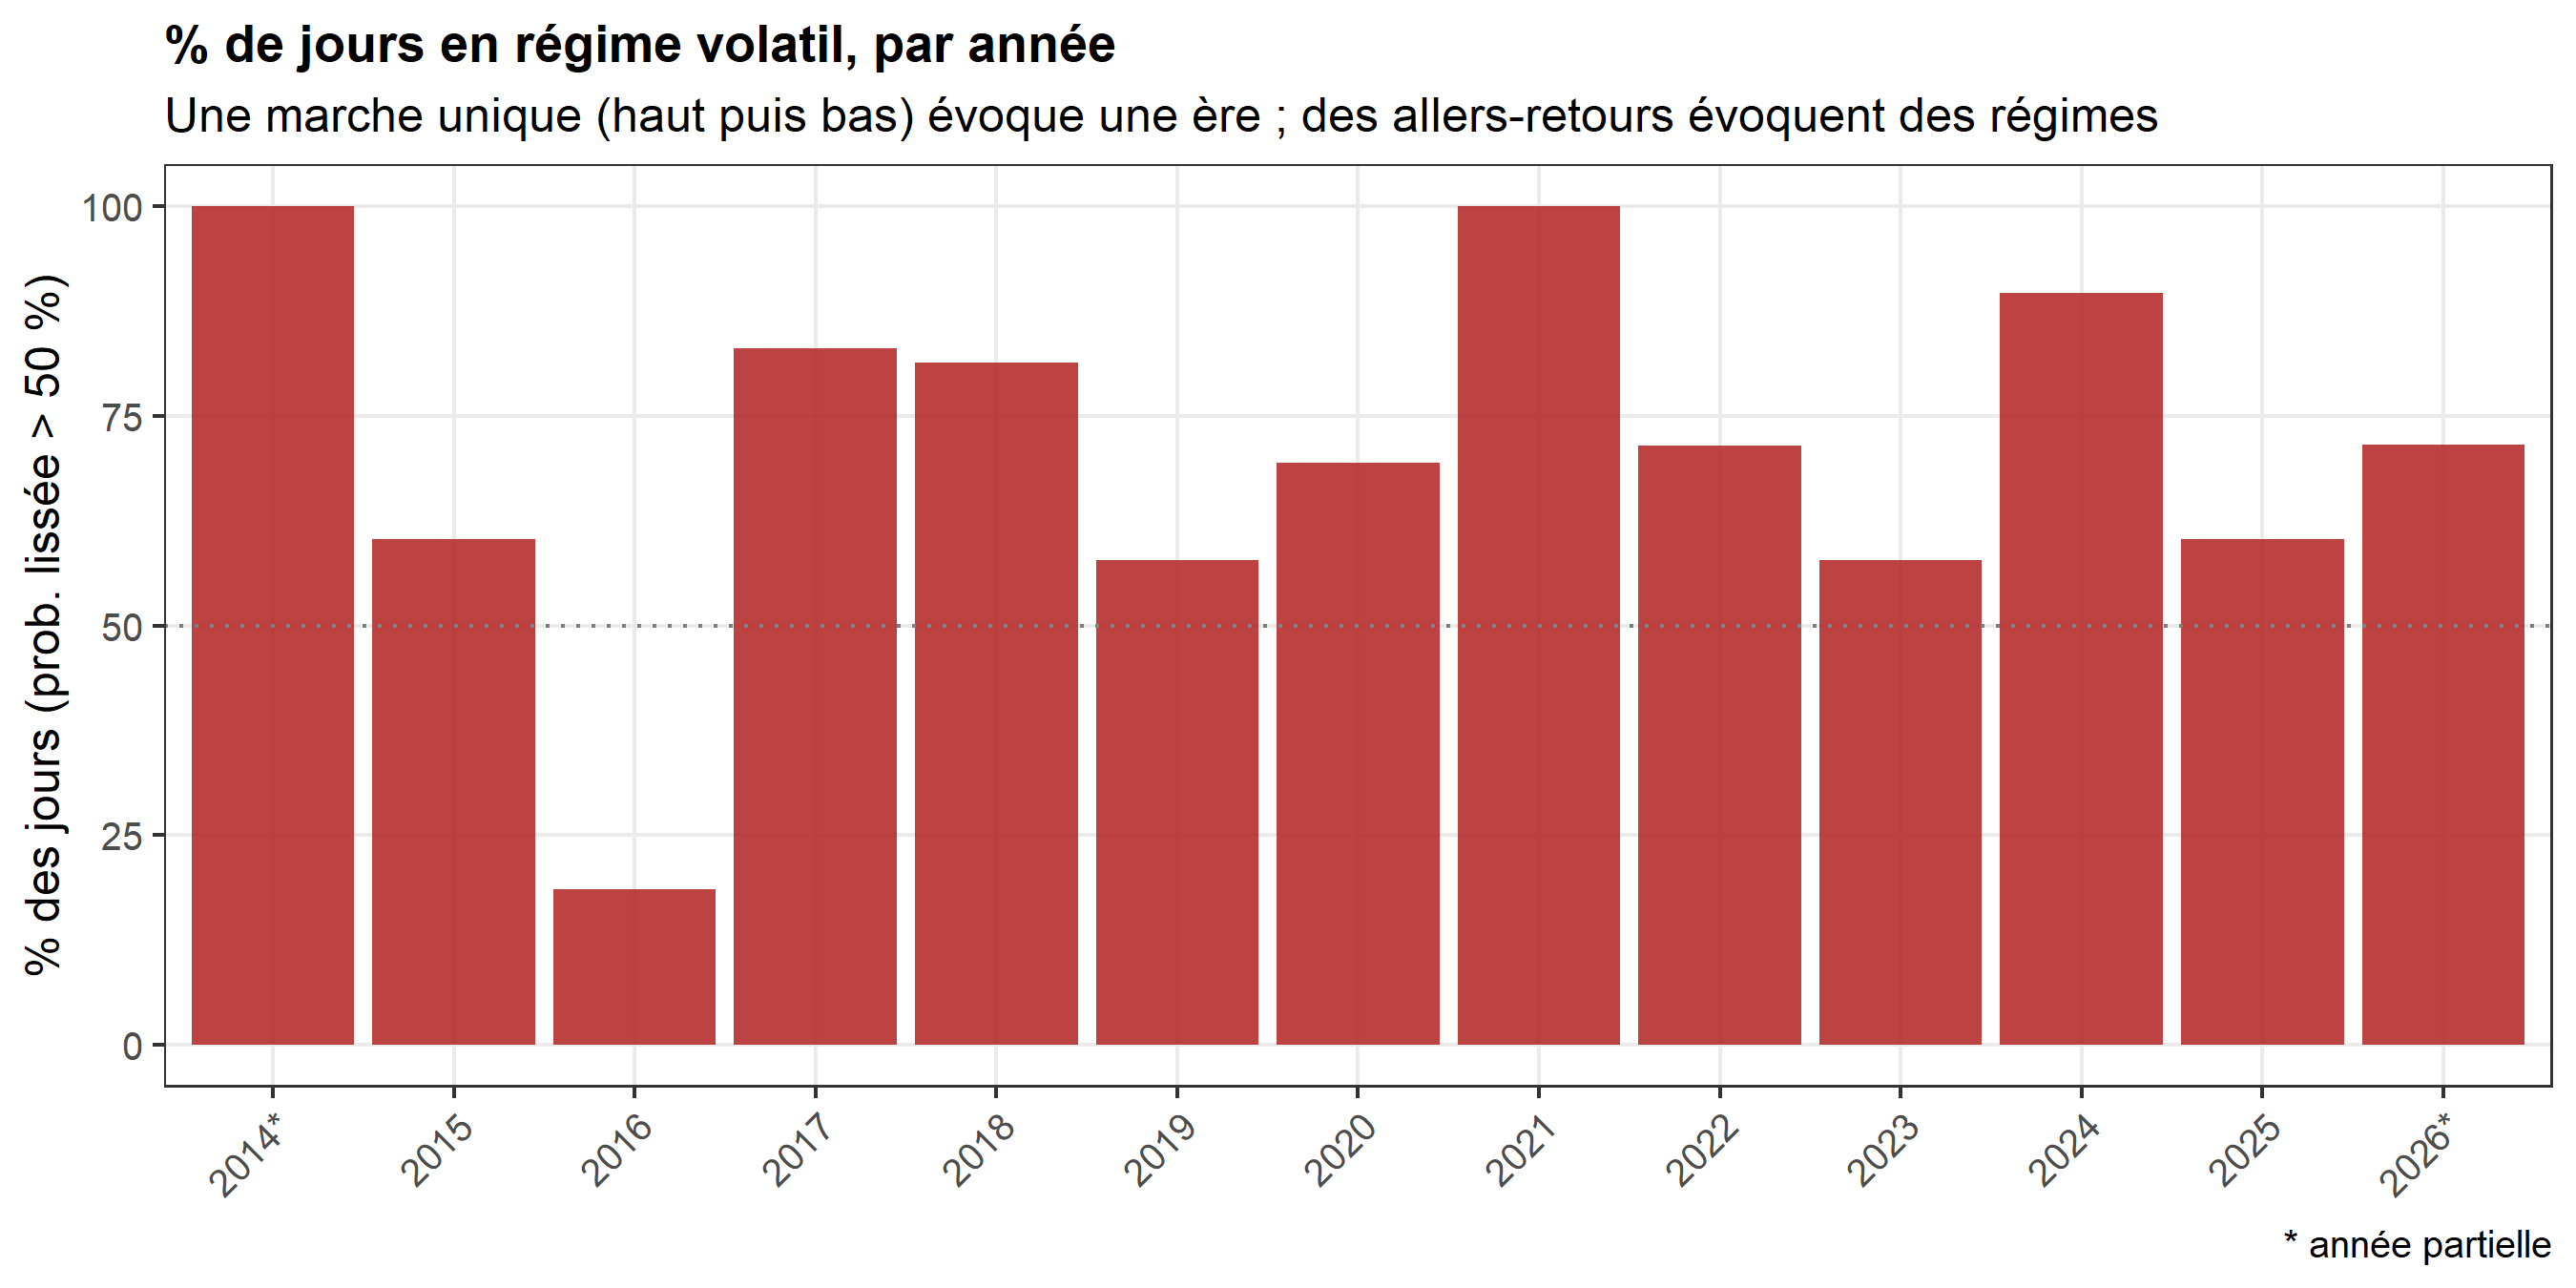
\includegraphics[width=1\linewidth]{05_yearly_highvol_pct.png}
	\caption{Share of days with a smoothed volatile-regime probability above $50\,\%$, by calendar year (2014 and 2026 are partial years). The share goes up and down, from about $19\,\%$ in 2016 to $100\,\%$ in 2021, with no single step: this is the pattern expected of regimes and not of an era. It does not follow the yearly standard deviation of Table~\ref{tab:data-yearly}. Figure labels are in French.}
	\label{fig:app-yearly}
\end{figure}

\subsection{Regime label and realised volatility}

\begin{figure}[H]
	\centering
	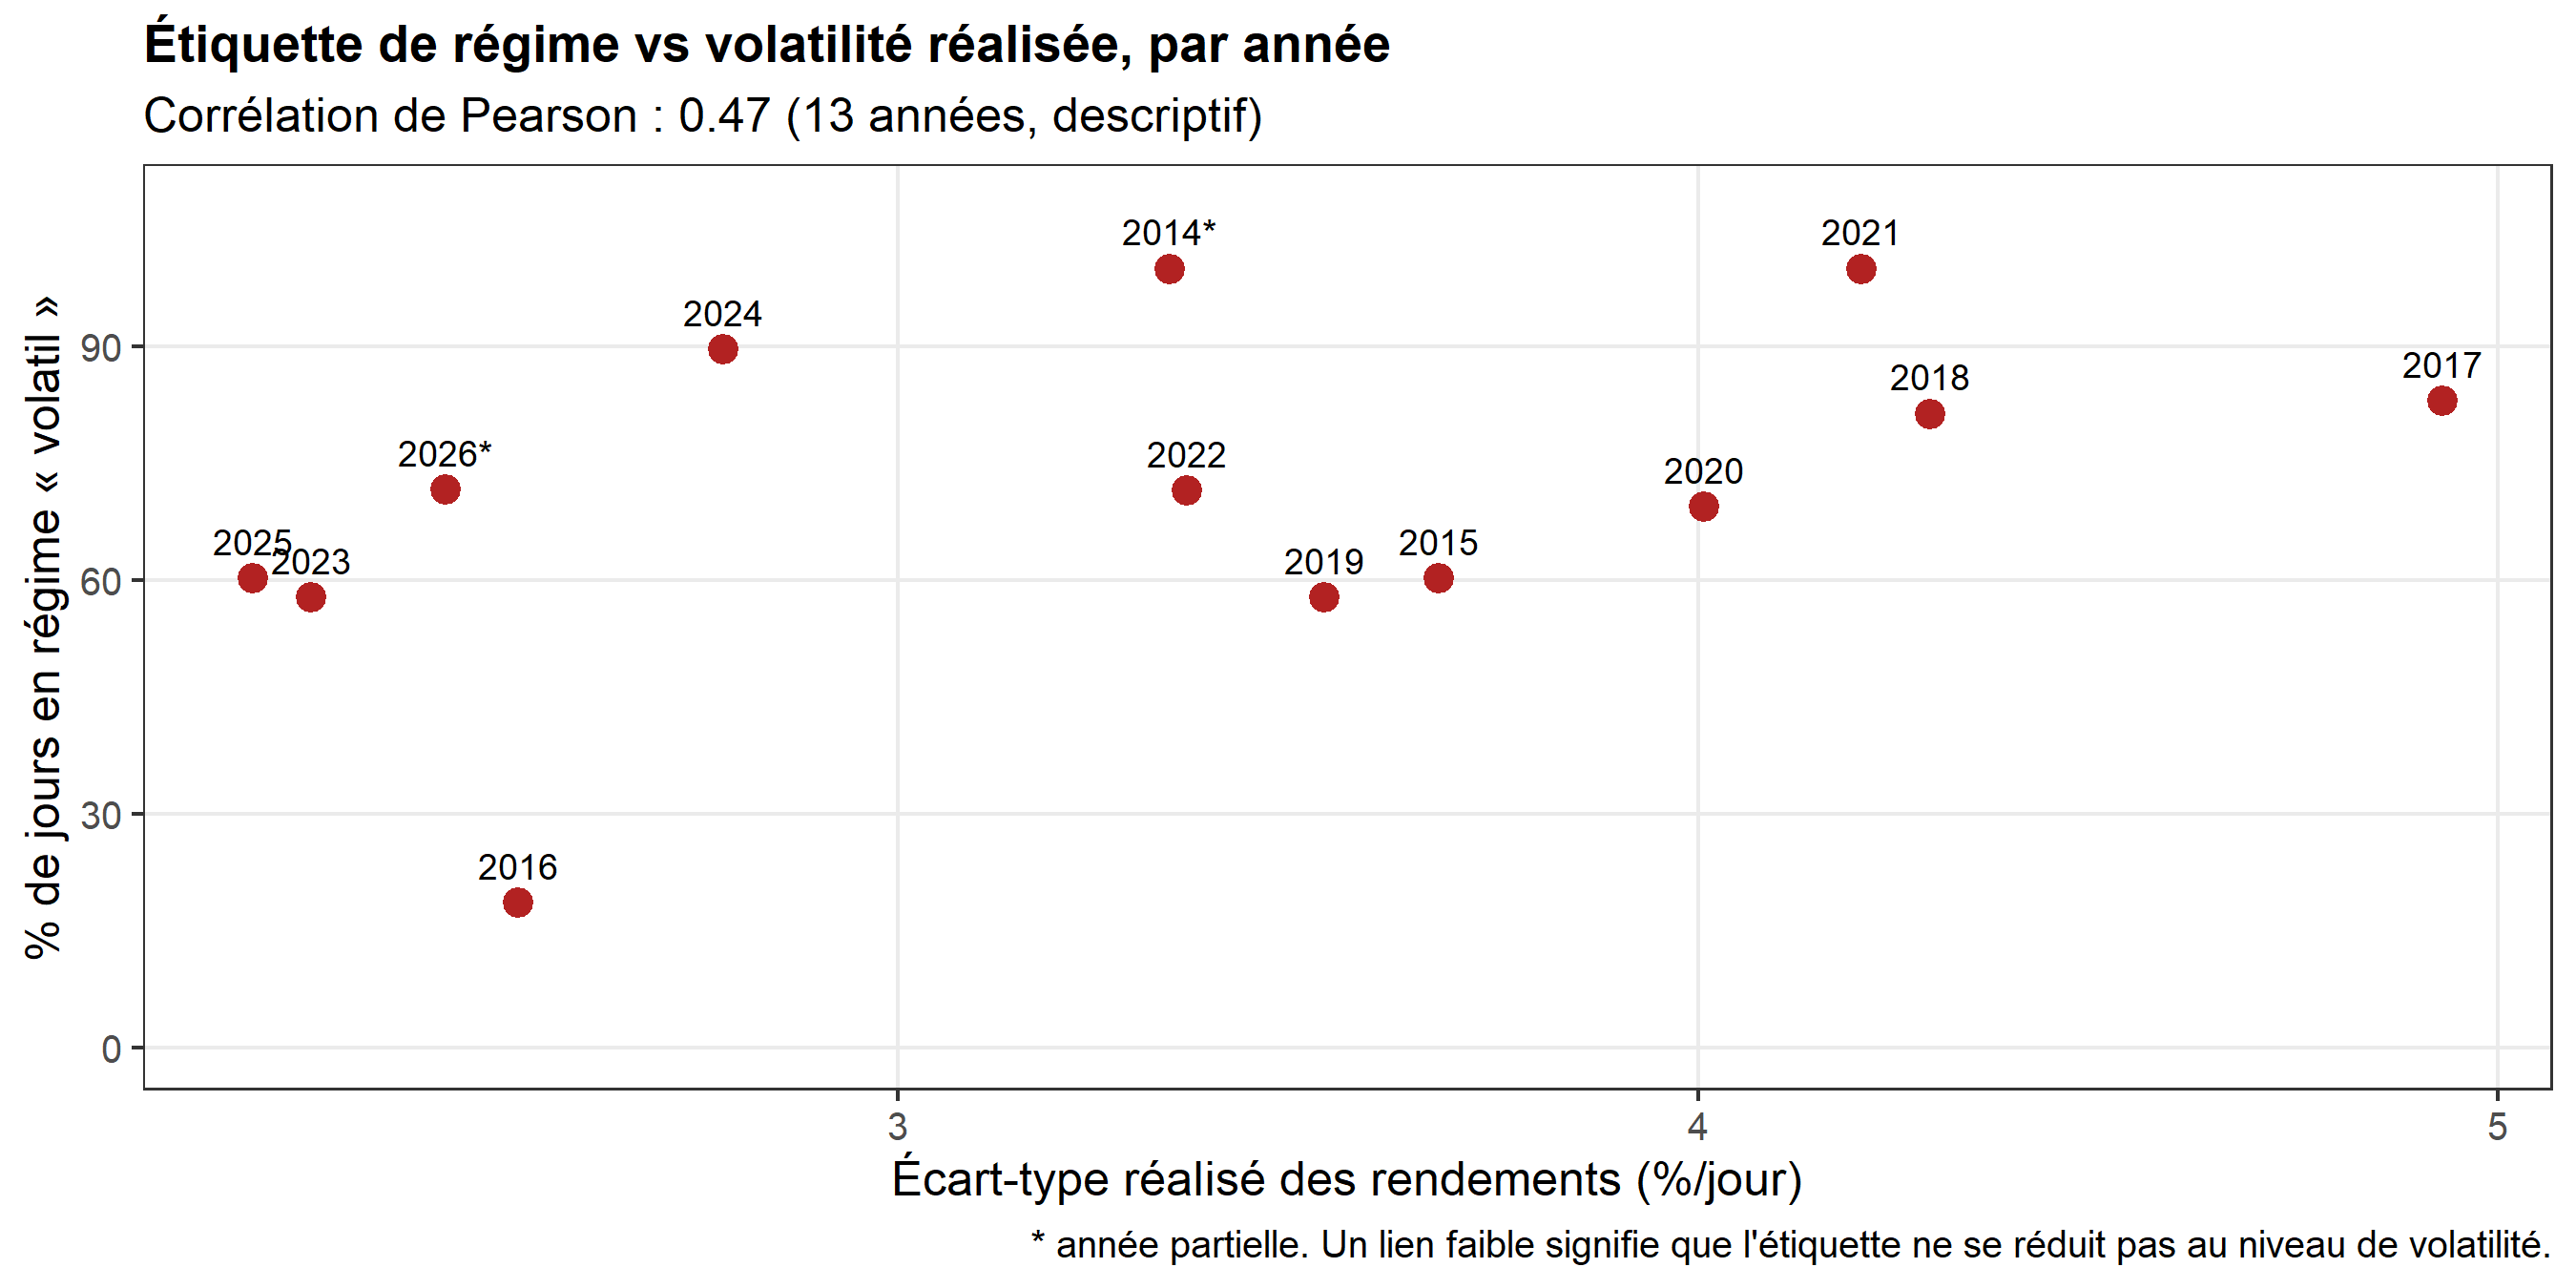
\includegraphics[width=1\linewidth]{09_label_vs_realized_vol_by_year.png}
	\caption{Share of days labelled ``volatile'' against the realised standard deviation of the returns, by calendar year (2014 and 2026 are partial years). The Pearson correlation is $0.47$ over 13 points, a descriptive figure: with so few points it is not significantly different from zero at the 5\,\% level. The label is related to the volatility level but does not reduce to it: 2016 and 2023 have similar standard deviations ($2.5\,\%$ and $2.3\,\%$) and very different shares of volatile days ($19\,\%$ and $58\,\%$). Figure labels are in French.}
	\label{fig:app-label-vol}
\end{figure}

\subsection{Returns by regime}

\begin{figure}[H]
	\centering
	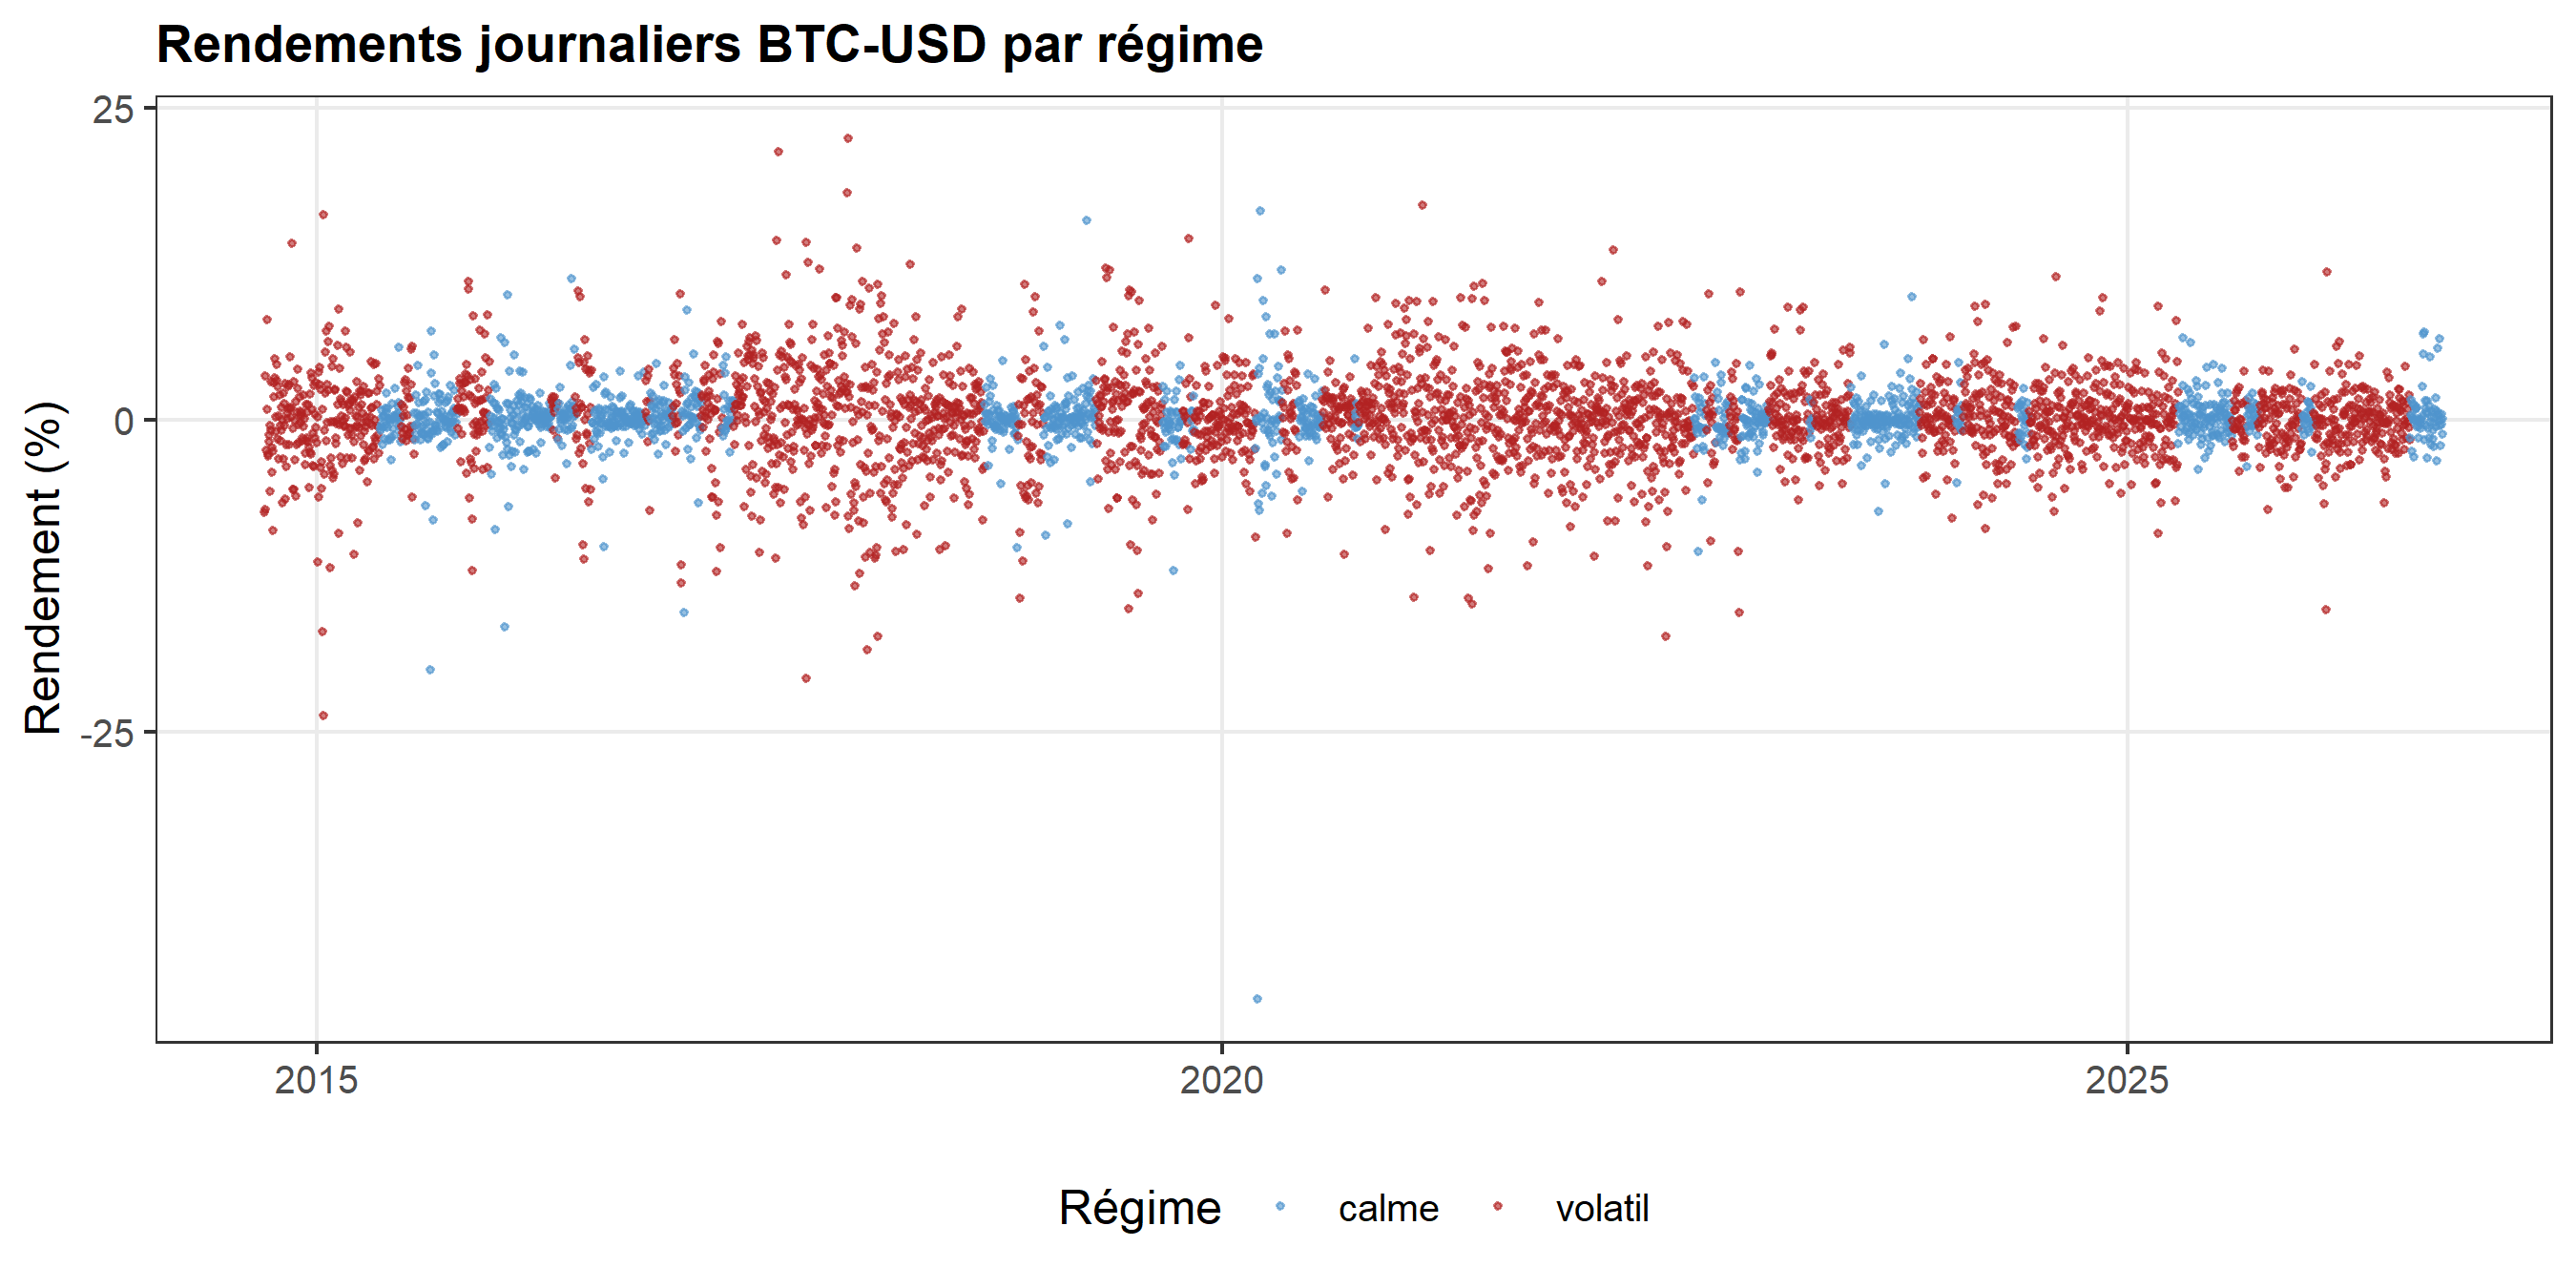
\includegraphics[width=1\linewidth]{07_returns_by_regime.png}
	\caption{Daily log returns coloured by regime (volatile or calm, according to the smoothed probability). The calm points have a narrow dispersion but include isolated extremes, among them the $-46.5\,\%$ of 2020-03-12. Figure labels are in French.}
	\label{fig:app-returns-regime}
\end{figure}

\subsection{Distribution of returns by regime}

\begin{figure}[H]
	\centering
	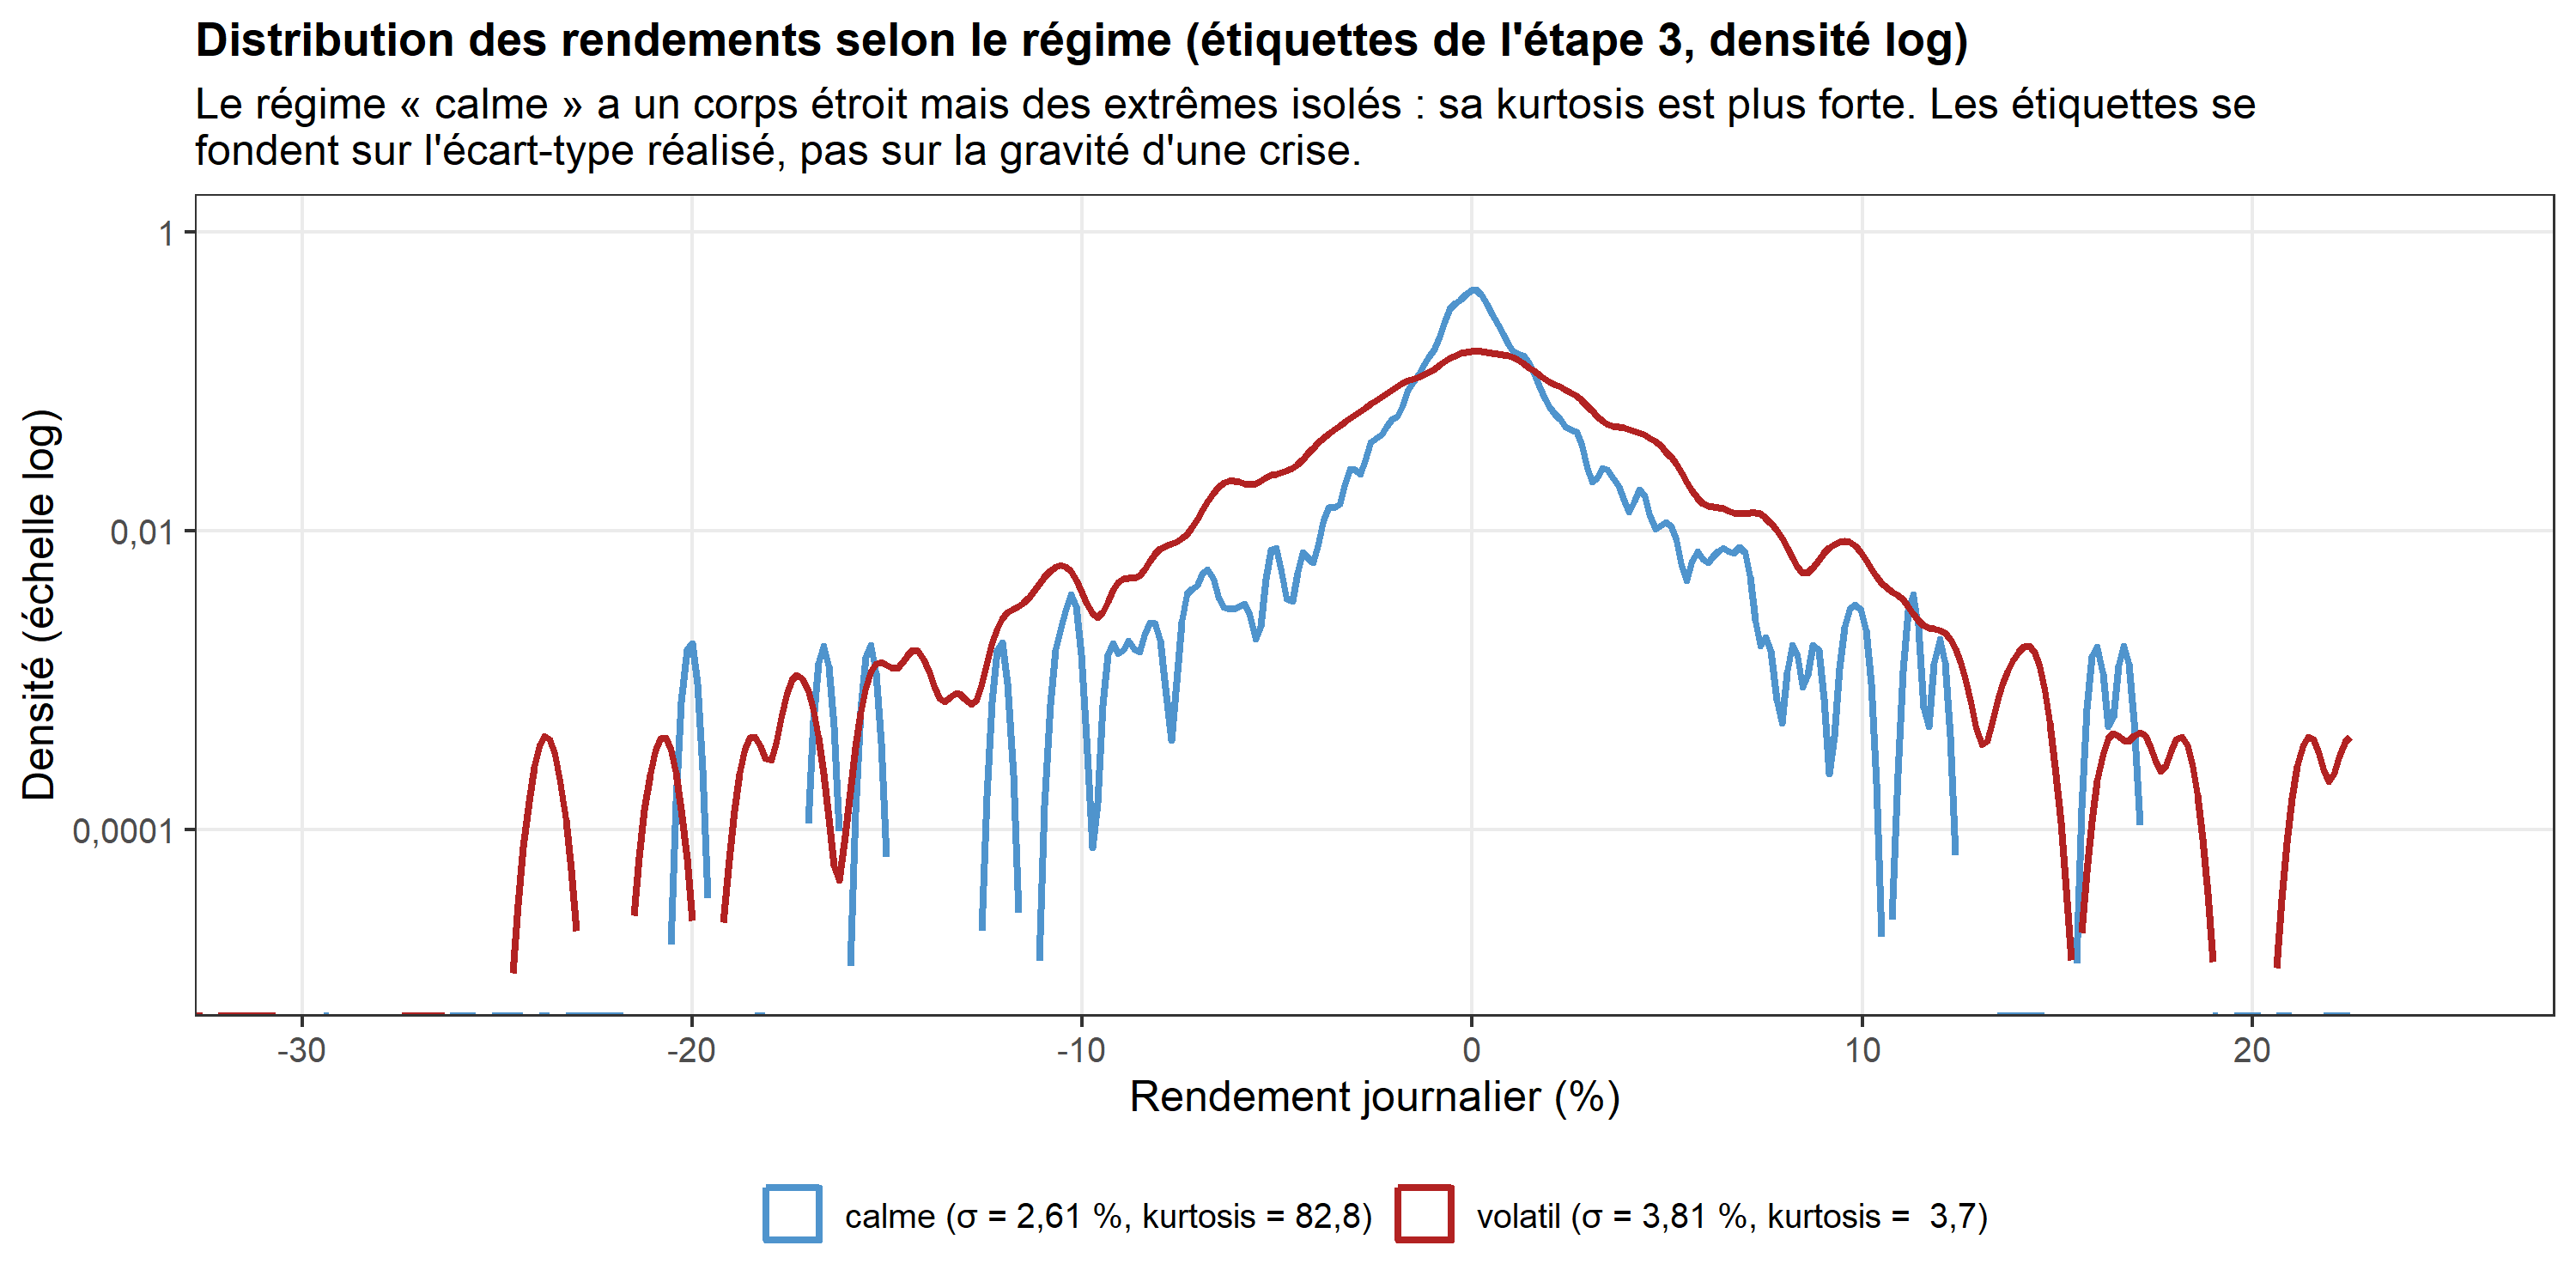
\includegraphics[width=1\linewidth]{D5_distribution_by_regime.png}
	\caption{Density of the returns of each regime, log scale. The calm regime has a narrow body but isolated extremes. The tails of both curves are jagged (a kernel estimate on few points) and are not interpreted. Figure labels are in French.}
	\label{fig:app-dist-regime}
\end{figure}

The excess kurtosis of the calm regime ($\approx 83$ on its 1,357 days, standard deviation $2.61\,\%$) is driven by a single day: without 2020-03-12 it falls to about $16$ and the standard deviation to $2.28\,\%$. The ``calm'' regime is therefore a set of ordinary days punctuated by jumps, which is consistent with its tail parameter ($\nu=2.30$).

\subsection{Tail index}

\begin{figure}[H]
	\centering
	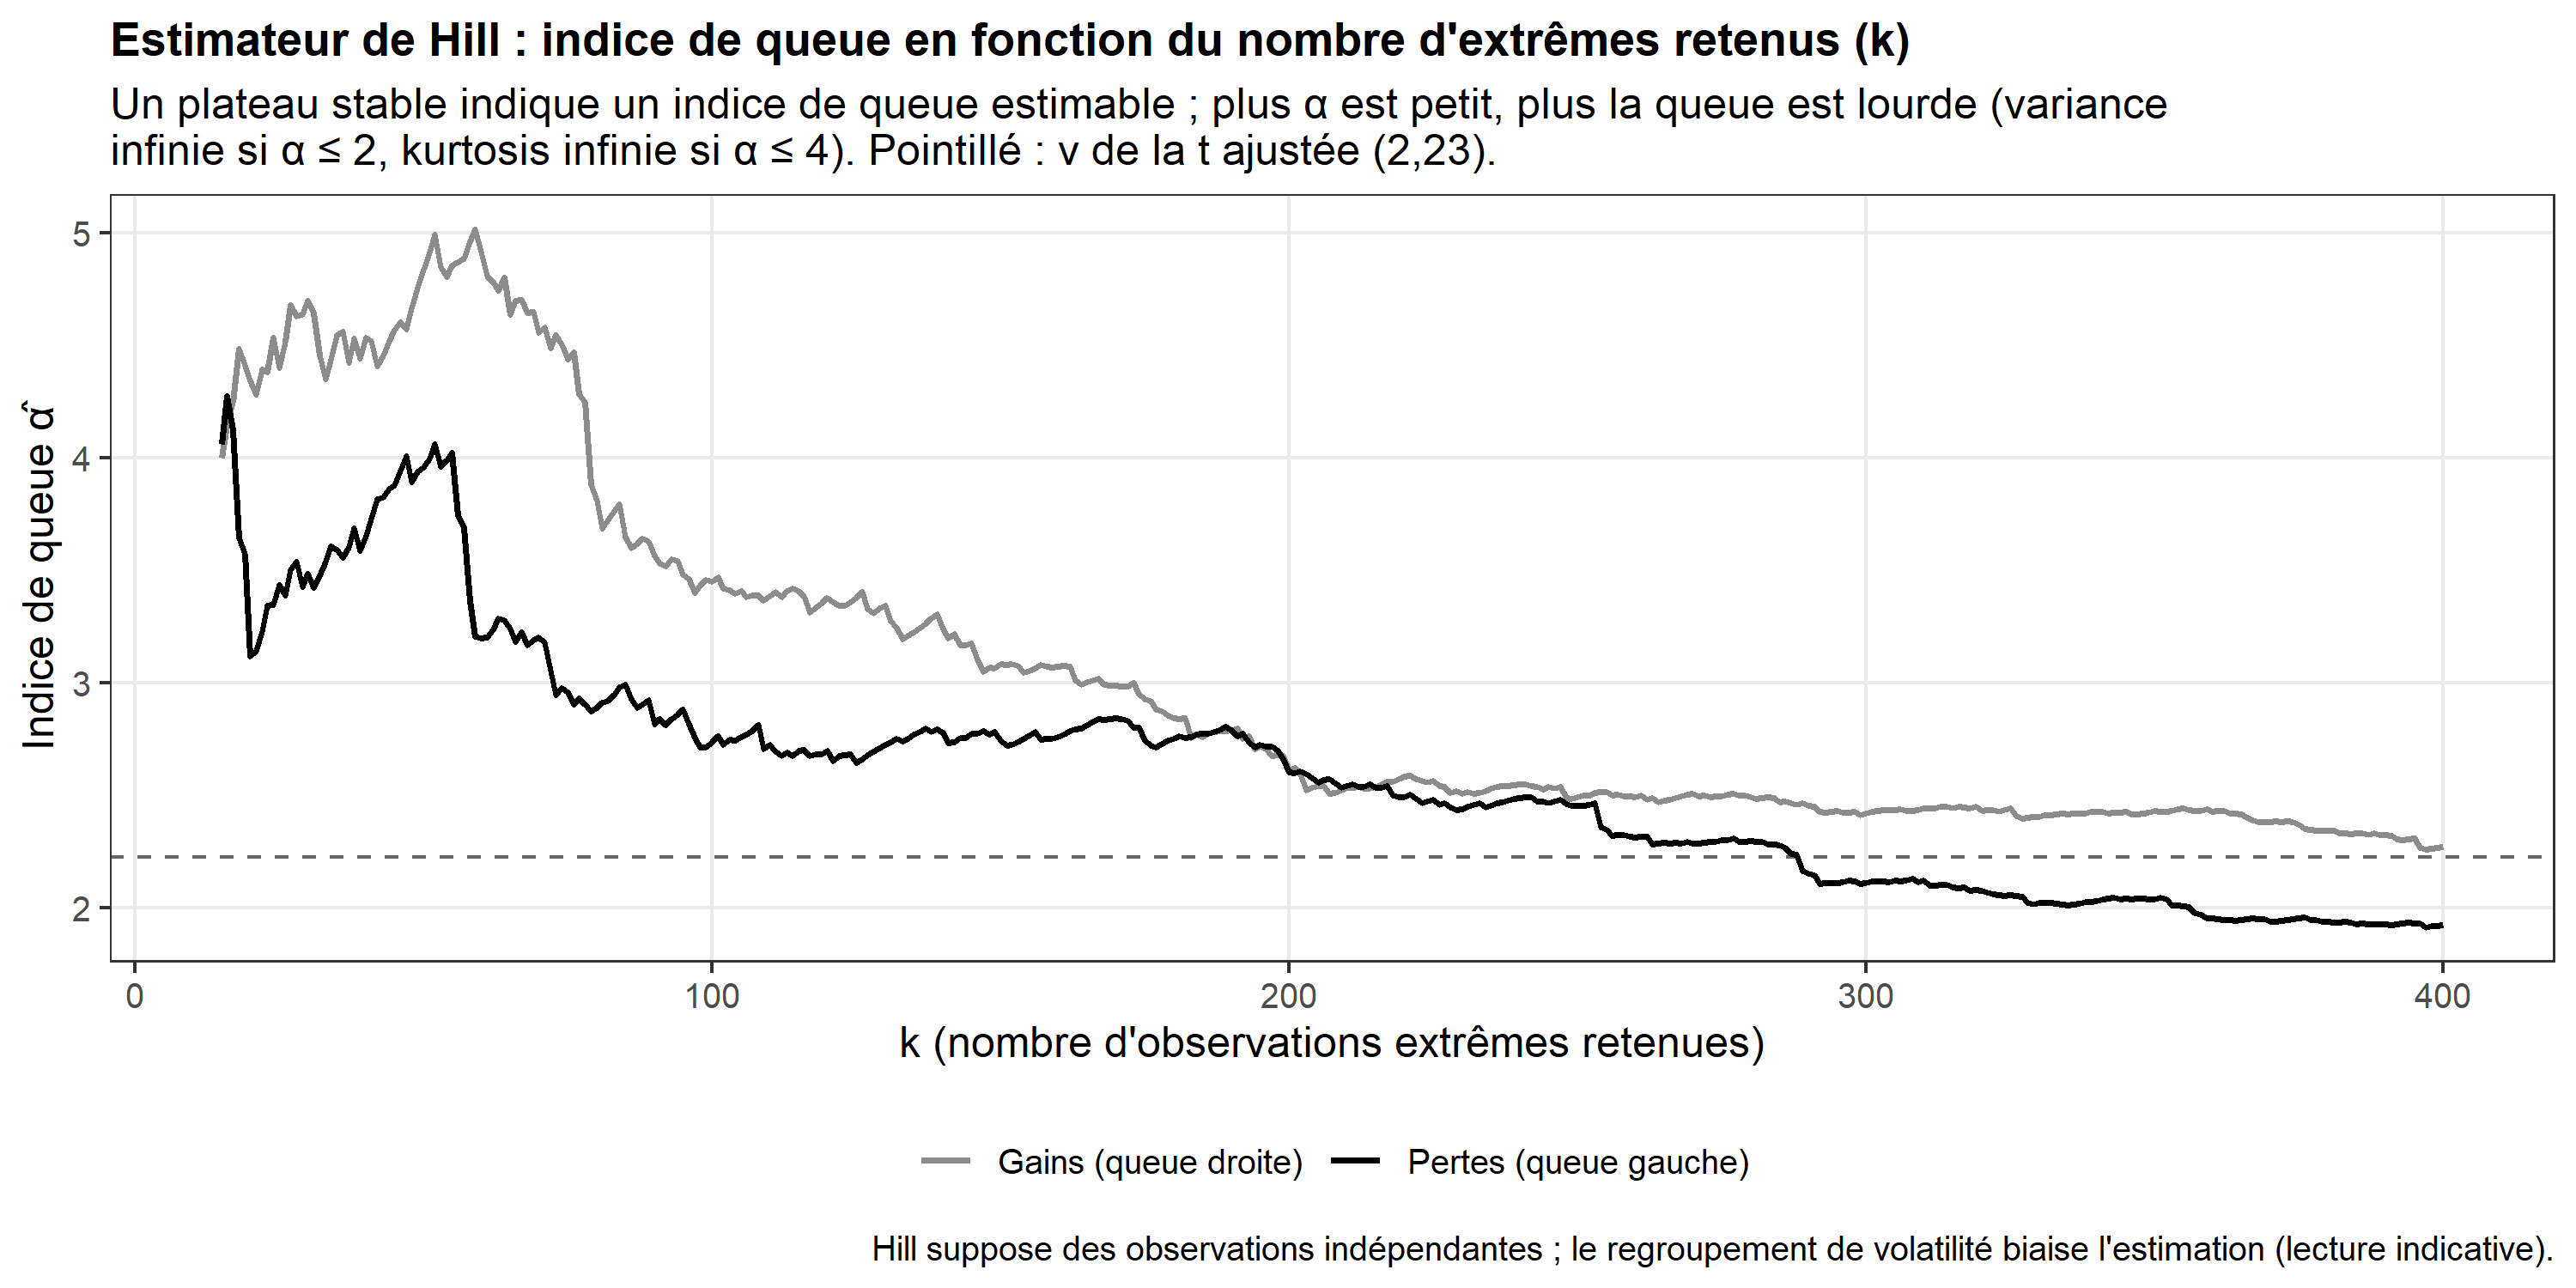
\includegraphics[width=1\linewidth]{D4_hill_plot.png}
	\caption{Hill estimator of the tail index $\hat\alpha$ as a function of the number $k$ of extreme observations retained, for losses (left tail) and gains (right tail); the dotted line is the $\nu$ of the fitted $t$ ($2.23$). There is \textbf{no plateau}: for losses the estimate moves from about $4$ at small $k$ to about $1.9$ at $k=400$, and for gains from about $5$ to about $2.3$. The tail index is therefore not identified, and no single value should be quoted. The Hill estimator assumes independent observations; volatility clustering biases it, so the reading is indicative. Figure labels are in French.}
	\label{fig:app-hill}
\end{figure}

% ═════════════════════════════════════════════════════════════════
\section{Traceability: results, output files and scripts}
\label{sec:app-trace}
% ═════════════════════════════════════════════════════════════════

Every figure quoted in the text comes from an output file, not from memory. The table below maps each block of results to the files and scripts that produce it; all of them are in the repository \url{https://github.com/Armando-ZEWU/BTC-Volatility-Regime-Model}.

\begin{table}[H]
	\centering
	\footnotesize
	\caption{From results to output files and scripts}
	\label{tab:trace}
	\raggedright
	\begin{tabular}{p{3.9cm}p{6.2cm}p{3.3cm}}
		\toprule
		Result & Output files & Script \\
		\midrule
		Returns, quality checks (Table~\ref{tab:data-quality}) & \texttt{btc\_\allowbreak{}close\_\allowbreak{}clean.csv}\newline \texttt{btc\_\allowbreak{}log\_\allowbreak{}returns.csv}\newline \texttt{btc\_\allowbreak{}usd\_\allowbreak{}yfinance\_\allowbreak{}raw.csv} & \texttt{data\_\allowbreak{}loading.py} \\
		\addlinespace
		GARCH, Normal vs $t$ (Table~\ref{tab:garch-results}) & \texttt{btc\_\allowbreak{}garch\_\allowbreak{}step2\_\allowbreak{}table.csv}\newline \texttt{btc\_\allowbreak{}garch\_\allowbreak{}shocks.csv} & \texttt{garch\_\allowbreak{}btc.py} \\
		\addlinespace
		MS-GARCH parameters, transition matrix, $K=1$ vs $K=2$ & \texttt{btc\_\allowbreak{}msgarch\_\allowbreak{}params\_\allowbreak{}flags.csv}\newline \texttt{btc\_\allowbreak{}msgarch\_\allowbreak{}transition\_\allowbreak{}matrix.csv}\newline \texttt{btc\_\allowbreak{}msgarch\_\allowbreak{}ic\_\allowbreak{}comparison.csv} & \texttt{ms\_\allowbreak{}garch\_\allowbreak{}btc.R} \\
		\addlinespace
		Restarts and optima (Table~\ref{tab:ms-runs}, Figure~\ref{fig:ms-optima}) & \texttt{btc\_\allowbreak{}msgarch\_\allowbreak{}restarts.csv}\newline \texttt{btc\_\allowbreak{}msgarch\_\allowbreak{}optima\_\allowbreak{}sensitivity.csv} & \texttt{ms\_\allowbreak{}garch\_\allowbreak{}btc.R} \\
		\addlinespace
		Regime probabilities, blocks, descriptives & \texttt{btc\_\allowbreak{}msgarch\_\allowbreak{}regime\_\allowbreak{}probs.csv}\newline \texttt{btc\_\allowbreak{}msgarch\_\allowbreak{}highvol\_\allowbreak{}runs.csv}\newline \texttt{btc\_\allowbreak{}msgarch\_\allowbreak{}regime\_\allowbreak{}descriptives.csv} & \texttt{ms\_\allowbreak{}garch\_\allowbreak{}btc.R} \\
		\addlinespace
		``Regime or era'' rule (Table~\ref{tab:era-rule}) & \texttt{btc\_\allowbreak{}msgarch\_\allowbreak{}era\_\allowbreak{}rule.csv} & \texttt{ms\_\allowbreak{}garch\_\allowbreak{}btc.R} \\
		\addlinespace
		\bottomrule
	\end{tabular}
\end{table}

\begin{table}[H]
	\centering
	\footnotesize
	\caption{From results to output files and scripts (continued)}
	\raggedright
	\begin{tabular}{p{3.9cm}p{6.2cm}p{3.3cm}}
		\toprule
		Result & Output files & Script \\
		\midrule
		Split-sample test and prediction (Tables~\ref{tab:chow}, \ref{tab:era-prediction}) & \texttt{btc\_\allowbreak{}chow\_\allowbreak{}garch\_\allowbreak{}table.csv}\newline \texttt{btc\_\allowbreak{}chow\_\allowbreak{}garch\_\allowbreak{}lr.csv} & \texttt{chow\_\allowbreak{}garch\_\allowbreak{}btc.py} \\
		\addlinespace
		One-day range for 2026-09-29 (Tables~\ref{tab:range-result}--\ref{tab:range-mixture}) & \texttt{btc\_\allowbreak{}price\_\allowbreak{}range\_\allowbreak{}output.csv}\newline \texttt{btc\_\allowbreak{}msgarch\_\allowbreak{}price\_\allowbreak{}range\_\allowbreak{}inputs.csv}\newline \texttt{btc\_\allowbreak{}msgarch\_\allowbreak{}regime\_\allowbreak{}conditional\_\allowbreak{}forecast.csv}\newline \texttt{btc\_\allowbreak{}msgarch\_\allowbreak{}mixture\_\allowbreak{}check.csv}\newline \texttt{btc\_\allowbreak{}msgarch\_\allowbreak{}fan\_\allowbreak{}chart\_\allowbreak{}inputs.csv} & \texttt{ms\_\allowbreak{}garch\_\allowbreak{}forecast\_\allowbreak{}btc.R}, \texttt{price\_\allowbreak{}range\_\allowbreak{}btc.py} \\
		\addlinespace
		Shock test, 2020 (Tables~\ref{tab:shock-pre2020}--\ref{tab:shock-breaches}) & \texttt{btc\_\allowbreak{}covid\_\allowbreak{}result.csv}\newline \texttt{btc\_\allowbreak{}covid\_\allowbreak{}summary.csv}\newline \texttt{btc\_\allowbreak{}covid\_\allowbreak{}intraday.csv}\newline \texttt{btc\_\allowbreak{}covid\_\allowbreak{}pre2020\_\allowbreak{}flags.csv} & \texttt{covid\_\allowbreak{}shock\_\allowbreak{}test\_\allowbreak{}btc.R}, \texttt{msgarch\_\allowbreak{}utils\_\allowbreak{}btc.R} \\
		\addlinespace
		Backtest, forecasts and summary (Tables~\ref{tab:bt-main}, \ref{tab:bt-folds}) & \texttt{btc\_\allowbreak{}backtest\_\allowbreak{}daily.csv}\newline \texttt{btc\_\allowbreak{}backtest\_\allowbreak{}summary.csv}\newline \texttt{btc\_\allowbreak{}backtest\_\allowbreak{}fold\_\allowbreak{}summary.csv}\newline \texttt{btc\_\allowbreak{}backtest\_\allowbreak{}params.csv}\newline \texttt{btc\_\allowbreak{}backtest\_\allowbreak{}fold\_\allowbreak{}YYYY.csv}\newline \texttt{btc\_\allowbreak{}backtest\_\allowbreak{}par\_\allowbreak{}YYYY.csv} & \texttt{full\_\allowbreak{}backtest\_\allowbreak{}btc.R}, \texttt{msgarch\_\allowbreak{}utils\_\allowbreak{}btc.R} \\
		\addlinespace
		Benchmarks, terciles, regression, breach size, direction (Tables~\ref{tab:bm-95}--\ref{tab:bm-direction}) & \texttt{btc\_\allowbreak{}verif\_\allowbreak{}benchmarks.csv}\newline \texttt{btc\_\allowbreak{}verif\_\allowbreak{}conditional\_\allowbreak{}terciles.csv}\newline \texttt{btc\_\allowbreak{}verif\_\allowbreak{}mincer\_\allowbreak{}zarnowitz.csv}\newline \texttt{btc\_\allowbreak{}verif\_\allowbreak{}breach\_\allowbreak{}size.csv}\newline \texttt{btc\_\allowbreak{}verif\_\allowbreak{}direction.csv} & \texttt{verification\_\allowbreak{}btc.R} \\
		\addlinespace
				Complementary statistics: Wilson interval, symmetry, tests by fold, homogeneity, direction counts & \texttt{btc\_\allowbreak{}backtest\_\allowbreak{}stats.csv} & \texttt{backtest\_\allowbreak{}stats\_\allowbreak{}btc.py} \\
		\addlinespace
		Realised standard deviation by regime and fold (Table~\ref{tab:bt-sigma}) & \texttt{btc\_\allowbreak{}sigma\_\allowbreak{}by\_\allowbreak{}regime\_\allowbreak{}by\_\allowbreak{}fold.csv} & \texttt{Sigma\_\allowbreak{}by\_\allowbreak{}regime\_\allowbreak{}by\_\allowbreak{}fold.R} \\
		\addlinespace
		\bottomrule
	\end{tabular}
\end{table}

The pre-2020 model of section~\ref{sec:shock} is the same fit as the 2020 fold of the backtest: its parameters are in \texttt{btc\_\allowbreak{}backtest\_\allowbreak{}par\_\allowbreak{}2020.csv} (and in \texttt{btc\_\allowbreak{}covid\_\allowbreak{}pre2020\_\allowbreak{}par.rds}).

% ═════════════════════════════════════════════════════════════════
\section{Corrections log}
\label{sec:app-log}
% ═════════════════════════════════════════════════════════════════

Corrections that changed a result or its reading are recorded here, not erased.

\begin{table}[H]
	\centering
	\small
	\caption{The three executions of the MS-GARCH estimation script}
	\label{tab:ms-runs}
	\begin{tabular}{lp{3.2cm}p{4.2cm}p{4.2cm}}
		\toprule
		Run & Starting points & Best log-lik. & Structure found \\
		\midrule
		v1 & default + 5 perturbed & $-10{,}713.36$ & Micro-regimes: expected durations $\approx 2$ and 6 days \\
		v2 & default + 15 perturbed & $-10{,}713.36$ (4 of 15) & Same: 2.2 and 5.8 days, 91\,\% ambiguous days \\
		v3 & default + 8 perturbed + 12 ``persistent regimes'' & $\mathbf{-10{,}708.78}$ (10 of 12 persistent starts, 0 of 8 perturbed) & \textbf{Persistent regimes: 72.8 and 35.9 days} \\
		\bottomrule
	\end{tabular}
\end{table}

\begin{enumerate}
	\item \textbf{A local optimum taken for the global one.} In run v2 the restarts clipped the transition probabilities to $[0.6,\,0.995]$: every starting point was a micro-regime start, and the micro-regime optimum ($-10{,}713.36$) was taken for the global one, although it lies 4.58 log-likelihood points below the best. Corrected in v3 by adding ``persistent regime'' starts and logit noise on the transition probabilities. The reading changed from regimes of 2 and 6 days to regimes of 73 and 36 days.
	\item \textbf{One-sided $p$-values read as two-sided.} The \texttt{Pr(>|t|)} column of \texttt{MSGARCH} is one-sided; it was read as two-sided. The two-sided value is twice the displayed one. Corrected in section~\ref{sec:msgarch}.
	\item \textbf{A missing forecast on a crisis day.} In the first run of the shock test, \texttt{Risk()} failed on 2020-03-14 and the first version of the script did not record the cause; the day was missing from the 121. The corrected script uses the exact mixture as a fallback. Coverage at 95\,\%: 5 breaches out of 120 days ($95.83\,\%$) became 5 out of 121 ($95.87\,\%$). The risk was real, because the missing day was a crisis day: with 6 or 7 breaches out of 121 the one-sided binomial $p$-value would have been $0.57$ or $0.40$.
	\item \textbf{Sample sizes of the two halves.} The split-sample test was first documented with 2,197 returns on each side; the cut is the median of the 4,395 prices, which gives 2,196 and 2,198 returns. Corrected in section~\ref{sec:era}.
	\item \textbf{The last row of the raw data file.} The documentation placed the in-progress bar on 2026-09-29. The file ends with 2026-09-28 followed by an in-progress bar of 2026-09-30, and has no row for 2026-09-29. The analysis sample, which ends on 2026-09-28, is unchanged (section~\ref{sec:data-pipeline}).
\end{enumerate}


\end{document}
